%% Paper I of the Gaussian Schmidt arrangement project.
%% Sources: the repository documents circle-classification.md,
%% euclidean-counting.md, hyperbolic-counting.md, involution.md,
%% class-formula-proof.md, circle-composition.md,
%% spherical-moduli-invariants.md (SS1-2), moduli-invariants.md,
%% first-power-descent.md, euclidean-moduli-invariants.md, phase-atlas.md.
%% Machine verification: see Appendix A and the scripts/ directory.
\documentclass[11pt]{amsart}

\usepackage{amsmath,amssymb,amsthm}
\usepackage{graphicx}
\usepackage{booktabs}
\usepackage{longtable}
\usepackage[hidelinks]{hyperref}
\usepackage[expansion=false]{microtype}

\graphicspath{{../../figures/}}

\allowdisplaybreaks

\numberwithin{equation}{section}

\theoremstyle{plain}
\newtheorem{theorem}{Theorem}[section]
\newtheorem{proposition}[theorem]{Proposition}
\newtheorem{lemma}[theorem]{Lemma}
\newtheorem{corollary}[theorem]{Corollary}
\newtheorem{conjecture}[theorem]{Conjecture}

\theoremstyle{definition}
\newtheorem{definition}[theorem]{Definition}
\newtheorem{example}[theorem]{Example}
\newtheorem{openproblem}[theorem]{Open problem}

\theoremstyle{remark}
\newtheorem{remark}[theorem]{Remark}

%% notation
\newcommand{\C}{\mathbb{C}}
\newcommand{\R}{\mathbb{R}}
\newcommand{\Q}{\mathbb{Q}}
\newcommand{\Z}{\mathbb{Z}}
\newcommand{\HH}{\mathbb{H}}
\newcommand{\Zi}{\Z[i]}
\newcommand{\Rhat}{\widehat{\R}}
\newcommand{\Chat}{\widehat{\C}}
\newcommand{\SL}{\mathrm{SL}}
\newcommand{\PSL}{\mathrm{PSL}}
\newcommand{\PGL}{\mathrm{PGL}}
\newcommand{\SU}{\mathrm{SU}}
\newcommand{\Gal}{\mathrm{Gal}}
\newcommand{\Cl}{\mathrm{Cl}}
\newcommand{\Pic}{\mathrm{Pic}}
\newcommand{\tr}{\operatorname{tr}}
\newcommand{\im}{\operatorname{Im}}
\newcommand{\re}{\operatorname{Re}}
\newcommand{\disc}{\operatorname{disc}}
\newcommand{\arccot}{\operatorname{arccot}}
\newcommand{\arcoth}{\operatorname{arcoth}}
\newcommand{\arccosh}{\operatorname{arccosh}}
\newcommand{\Sarr}{\mathcal{S}}
\newcommand{\ideala}{\mathfrak{a}}
\newcommand{\idealb}{\mathfrak{b}}
\newcommand{\idealc}{\mathfrak{c}}
\newcommand{\idealm}{\mathfrak{m}}
\newcommand{\idealr}{\mathfrak{r}}
\newcommand{\ideals}{\mathfrak{s}}
\newcommand{\GZ}{\mathrm{GZ}}
\newcommand{\Res}{\operatorname{Res}}
\newcommand{\sgn}{\operatorname{sign}}
\newcommand{\lat}[1]{\left[#1\right]}

\begin{document}

\title[Schmidt circles of the Gaussian integers]{Schmidt circles of the
Gaussian integers:\\ classification, class numbers, and the phase invariant}

%% TODO before submission: complete author name and affiliation.
\author{Karl Ivar}
\email{karlivar2004@gmail.com}

\begin{abstract}
The Gaussian Schmidt arrangement is the orbit of the extended real line
under the Bianchi group, $\Sarr = \PSL_2(\Zi)\cdot\Rhat$: an arrangement
of circles first drawn by Asmus Schmidt and studied by Stange.  We develop its arithmetic in three layers.  First, starting from
the elementary congruence classification of its circles, we stratify
$\Sarr$ by an integer level $\alpha$ --- simultaneously the hyperbolic
radius invariant $\coth\rho$, a trace on the Cartan embedding
$X \mapsto X\bar X^{-1}$, and the inversive product with $\Rhat$ --- and
count the arrangement in its three background geometries: per unit area the
circles of curvature $2n$ number
$N_e(n) = n\prod_{p \mid n}(1 - \chi_{-4}(p)/p) = 2h(-4n^2)$, with mean
value governed by Catalan's constant; the circles of level $n$ in an ideal
triangle of the hyperbolic plane have weighted count $3H(n^2-1)$; and on
the Riemann sphere the circles of spherical radius $\arccot\ell$ number
$\tfrac13 r_3(\ell^2+1) = 4H(4(\ell^2+1))$.  Second, we identify the
involution $\sigma(X) = \bar X^{-1}$ as the unitary involution adjoint to
the Hermitian form of $\Rhat$, its Cartan image as the inversion in the
circle $X(\Rhat)$, and prove the class formula: on the primitive form
classes of discriminant $1-n^2$ attached to level-$n$ circles, $\sigma$
acts by $[f] \mapsto [\idealr_n][f]^{-1}$ for a canonical ambiguous class
$\idealr_n$ --- formally the Atkin--Lehner involution on Heegner points ---
and Gauss composition itself becomes a geometric calculus of mirrors and
magnifications of circles.  Third, we construct the sixth coordinate on the
double-coset space $\SL_2(\Z)\backslash\SL_2(\C)/\SL_2(\Z)$ --- a phase ---
and show that on Schmidt circles it quantizes: the normalized phase $u_f$
equals the derivative $\Phi_y/\Phi_x(\beta_1, \beta_2)$ of the modular
correspondence $X_0(\tfrac{n-1}{2})$ at a Heegner pair whose discriminant
is coupled to the level, obeys a generalized dihedral Galois law at first
power, and generates one integer polynomial per level, irreducible at every
computed level, with denominators supported at Gross--Zagier primes; on
ambiguous divisor classes its sign obeys a proved archimedean law and is
provably not a genus character.  A parallel Euclidean theory (translations
in place of one modular factor), normalized by the lemniscatic period,
produces monic integer level polynomials irreducible for \emph{every}
level, and an exact $\Delta$-mass law.  Certified high-precision
computations show the phase is not a rational linear combination of the
Duke--Imamo\u{g}lu--T\'oth cycle-integral invariants of its coupled real
quadratic discriminant: the phase appears to be a genuinely new invariant.
Every finite claim in the paper is machine-verified; the scripts and
precision policies are catalogued in an appendix.
\end{abstract}

\maketitle
\tableofcontents

%%% ============================================================
\section{Introduction}\label{sec:intro}

Let $\Gamma_{\mathrm{B}} = \PSL_2(\Zi)$ act on
$\Chat = \C \cup \{\infty\}$ by M\"obius transformations.  The
\emph{Gaussian Schmidt arrangement} is the orbit of the extended real
line,
\begin{equation}\label{eq:Sdef}
  \Sarr \;=\; \Gamma_{\mathrm{B}} \cdot \Rhat ,
\end{equation}
a countable union of circles and lines that first appeared, as the
boundary data of a complex Farey subdivision, in Asmus Schmidt's theory of
complex continued fractions \cite{Schmidt1975}, and whose systematic study
was begun by Stange \cite{StangeTAMS, StangeIMRN}: for an arbitrary
imaginary quadratic field the analogous orbit is an intricate circle
arrangement whose tangencies, curvatures and connectivity encode the
arithmetic of the field, and for $\Q(i)$ it coincides, up to scaling, with
the Apollonian super-packing of Graham, Lagarias, Mallows, Wilks and Yan
\cite{GLMWY2006, StangeTAMS}.  Figure~\ref{fig:atlas9} shows a portion.

This paper develops the arithmetic of $\Sarr$ in three layers, of
increasing depth.

\subsection*{First layer: classification and three censuses}
The circles of $\Sarr$ admit an elementary Diophantine description
(Theorem \ref{thm:classification}; in equivalent forms this is known
\cite{GLMWY2006, StangeTAMS, RickardsStange2026}): a circle of radius
$\tfrac1{2n}$ centered at $\zeta/2n$ belongs to $\Sarr$ if and only if
$\zeta = x + iy \in \Zi$ with $x$ even, $y$ odd and
$x^2 + y^2 \equiv 1 \pmod{4n}$ --- all conditions together amounting to the
single Diophantine equation $u^2 + v(v+1) = nm$.  Our starting point is a
stratification of $\Sarr$ that does not appear in the literature: the
integer
\[
  \alpha \;=\; \frac{\text{height of center}}{\text{radius}}
\]
of a circle in the upper half-plane, which is simultaneously
$\coth$ of its hyperbolic radius, the trace invariant
$-\tfrac12\tr(X\bar X^{-1})$ of the Cartan embedding, and the inversive
product of the circle with $\Rhat$ (Proposition \ref{prop:level}).  The
level-$n$ circles are in explicit bijection with the positive definite
binary quadratic forms of discriminant $1 - n^2$, their hyperbolic centers
are the CM points of that discriminant, and their hyperbolic radius
$\arcoth n$ depends on the level alone (Proposition
\ref{prop:formdictionary}).

Counting the arrangement then produces class numbers in each of the three
classical geometries carried by $\Chat$ (Theorem \ref{thm:triptych}): per
unit area of $\C$ the circles of curvature $2n$ number
\[
  N_e(n) = n\prod_{p \mid n}\Bigl(1 - \frac{\chi_{-4}(p)}{p}\Bigr)
  = 2\,h(-4n^2),
  \qquad
  \sum_{n \le X} N_e(n) = \frac{X^2}{2G} + O(X\log X),
\]
with $G = L(2, \chi_{-4})$ \emph{Catalan's constant} (Propositions
\ref{prop:Ne}--\ref{prop:catalan}; the class-number form of the count is,
for $\Q(i)$, a theorem of Stange \cite{StangeIMRN}, which we reprove
through an explicit lattice dictionary used heavily later); the circles of
level $n$ whose hyperbolic center lies in the ideal triangle
$(0, 1, \infty)$, counted with weight $\tfrac12$ on the edges, number
$3H(n^2 - 1)$, where $H$ is the Hurwitz class number (Theorem
\ref{thm:hyperbolic}); and on the Riemann sphere the spherical radii
quantize to the integer-cotangent angles $\cot\theta = \ell$, with exactly
\[
  N_{\mathrm{sph}}(\ell) = \tfrac13\, r_3(\ell^2 + 1) = 4H(4(\ell^2+1))
\]
circles of spherical radius $\arccot \ell$ (Theorem \ref{thm:spherical}).
One arrangement, three geometries, three class-number censuses; the
hyperbolic and spherical counts read the Hurwitz--Cohen--Eisenstein
weight-$3/2$ coefficients along the two quadratic progressions
$d = n^2 - 1$ and $d = 4\ell^2 + 4$, complementary to the Euclidean
$d = 4n^2$.

\subsection*{Second layer: the involution and the class formula}
The map $\sigma(X) = \bar X^{-1}$ is the adjoint anti-involution of the
Hermitian form defining $\Rhat$ --- a unitary involution, of the second
kind, on $M_2(\Q(i))$ --- and its Cartan image $X\bar X^{-1}$ is,
exactly, the anti-holomorphic inversion in the circle $X(\Rhat)$
(Theorem \ref{thm:cartan}); the trace identity
$\tr(X\bar X^{-1}) = -2\alpha$ recovers the level and attaches to every
level-$n$ circle a closed geodesic of length $2\arccosh n$ in the Bianchi
orbifold.  On the level-$n$ form classes, $\sigma$ induces an involution
$\hat\sigma$, and our first main arithmetic result computes it
(Theorem \ref{thm:classformula}): on primitive classes
\[
  \hat\sigma[f] \;=\; [\idealr_n]\,[f]^{-1},
  \qquad
  \idealr_n = \Bigl[\Bigl(\tfrac{n-1}{2},\,0,\,\tfrac{n+1}{2}\Bigr)\Bigr],
\]
a Galois conjugation of the class group twisted by a canonical ambiguous
class --- formally identical to the Atkin--Lehner action
$[\ideala] \mapsto [\mathfrak{n}\bar\ideala]$ on Heegner points.  The
proof runs through an explicit closed-form section (Lemma
\ref{lem:lemmaA}): a formula producing, for every prescribed level-$n$
circle, a matrix $X \in \SL_2(\Zi)$ realizing it --- a tool we expect to
be of independent use.  Composition of forms itself becomes visible in the
arrangement: the inverse of a circle class is its mirror image, Gauss
composition is a Chinese-remainder gluing characterized by integer
magnifications, and $2$-torsion classes are exactly the circles with a
mirror symmetry (Section \ref{sec:composition}).

\subsection*{Third layer: the phase}
The pair of circles $(X(\Rhat), \sigma(X)(\Rhat))$ has five real
invariants under $X \mapsto \gamma X \gamma'$,
$\gamma, \gamma' \in \SL_2(\Z)$: the level $\alpha$ and the two singular
moduli $\beta_1, \beta_2$ at the hyperbolic centers.  The sixth
coordinate on the double-coset space
$\SL_2(\Z)\backslash\SL_2(\C)/\SL_2(\Z)$ is a \emph{phase}
$\Theta(X)$, built from a weight-$2$ kernel and the derivative of $X$ at
a distinguished intertwined CM point (Section \ref{sec:phase}).  On the
Bianchi group this continuous invariant quantizes to algebraic numbers
$u_f = \varepsilon\,\Theta_f$, $\varepsilon = n + \sqrt{n^2-1}$, indexed
by the form classes of the level, and obeys the exact laws
$u_{f^{-1}} = \bar u_f$ and $u_f\,u_{\idealr_n f} = 1$.  The pair
$(\beta_1, \beta_2)$ of a class and its twist satisfies the
\emph{simultaneous modular equations}
$\Phi_{(n-1)/2}(\beta_2, \bar\beta_1) = 0 =
\Phi_{(n+1)/2}(\beta_2, \bar\beta_1)$: each $\hat\sigma$-pair of Schmidt
circles is a point on the fiber product
$X_0(\tfrac{n-1}{2}) \times_{X(1)} X_0(\tfrac{n+1}{2})$ whose
discriminant is coupled to its level --- and the phase is precisely the
derivative of this correspondence at its Heegner pair:
\[
  u_f \;=\; \frac{\Phi_y(\beta_1, \beta_2)}{\Phi_x(\beta_1, \beta_2)},
  \qquad \Phi = \Phi_{(n-1)/2}
\]
(Theorem \ref{thm:firstpower}).  Because the right-hand side is a rational
expression with rational coefficients in two singular moduli, the Galois
action on $u_f$ is completely transparent: $u_f$ lies in the ring class
field of discriminant $1 - n^2$ and transforms under the full generalized
dihedral law \emph{at first power}, with no root-of-unity cocycle
(Theorem \ref{thm:dihedral}).  Consequences: the $h$ phases of a level are
the roots of a single integer polynomial $Q_n$ of degree $h(1-n^2)$,
irreducible at every computed level $n \le 17$ (Theorems
\ref{thm:levelpoly}--\ref{thm:pin-irred}); the denominators of $u_f$ are
supported at the Gross--Zagier primes of the discriminant pairs
$(1-n^2, -3)$ and $(1-n^2, -4)$ --- the primes where the level's CM points
collide with the two elliptic points of the modular orbifold (Section
\ref{subsec:gz}); and on ambiguous divisor classes the \emph{sign} of
$u_f$ obeys a proved archimedean law --- a gcd inequality reading off on
which side of the $E_6$-zero the twisted CM point falls --- and is
provably \emph{not} a homomorphism on $\Cl[2]$ (Theorem \ref{thm:signlaw},
Proposition \ref{prop:notcharacter}).

A parallel \emph{Euclidean} phase theory, in which the left
$\SL_2(\Z)$-factor is replaced by the translations $\Zi$, is developed in
Section \ref{sec:euclidean}: there the level's CM data is the ring class
field of the order $\Z + n\Zi$ (conductor equal to the level, field
fixed), the phase is normalized by the lemniscatic period
$\Omega = \varpi^2/\pi$, and the theory is complete in a way the
hyperbolic one is not yet: the level polynomials are \emph{monic} with
integer coefficients, and are irreducible \emph{for every level}
(Theorem \ref{thm:euclideanirred}), by a cocycle-free Shimura translation
law at square level and an archimedean dominance argument; moreover the
total $\Delta$-mass of a level obeys an exact product law over the
non-split primes (Theorem \ref{thm:massa}).

\subsection*{What is new, and what is not}
The classification of Section \ref{sec:classification} is essentially
known: curvature integrality and the Hermitian framework are Stange's
\cite{StangeIMRN}, and the congruence description is equivalent to the
strongly-integral super-packing description of \cite{GLMWY2006} combined
with the identification of $\Sarr$ with the super-packing
\cite{StangeTAMS}; a congruence form is stated in
\cite{RickardsStange2026}.  We include a short self-contained proof to fix
normalizations and because the descent it sets up is used throughout.
Likewise the Euclidean census in its class-number form specializes a
theorem of Stange \cite{StangeIMRN}.  Everything else, to the best of our
knowledge --- the level stratification and the hyperbolic and spherical
censuses, the identification of $\sigma$ and the class formula, the
circle calculus of composition, the six-coordinate moduli system, the
phase and all its laws, and the Euclidean phase theory --- is new.  Three
literature probes are recorded in the repository accompanying this paper;
beyond the Schmidt-arrangement literature proper
\cite{Schmidt1975, StangeTAMS, StangeIMRN, RickardsStange2026,
Martin2022}, the objects closest in spirit are the cycle-integral
invariants of real quadratic discriminants of Duke, Imamo\u{g}lu and
T\'oth \cite{DIT2011} attached, through the Katok--Sarnak correspondence
\cite{KatokSarnak1993}, to the same coupled discriminant pairs
$(1-n^2,\, 4(n^2-1))$ that index our phase.  This proximity can be tested:
at levels $3 \le n \le 17$, certified integer-relation searches at
$150$-digit precision (with conservative safety margins) find \emph{no}
rational linear relation between $\log|u_f|$, $\arg u_f$ or the pair-sums
$u_f + u_f^{-1}$ and the discriminant-$4(n^2-1)$ cycle integrals of $j$,
the Kronecker-limit integrals, $\log\varepsilon_n$, $\pi$, $\pi^2$ and
$1$ (Section \ref{subsec:dit}).  The phase is, as far as we can measure,
genuinely new real-quadratic-adjacent data.

\subsection*{Status conventions}
Every statement below is one of two kinds, and the distinction is
maintained explicitly.  A \textbf{Theorem}, \textbf{Proposition},
\textbf{Lemma} or \textbf{Corollary} without qualification is proved.  A
statement labelled \emph{(computational)} is a finite claim verified by
exact arithmetic, or a numerical claim certified at a stated precision
with stated safety margins, by a named script; the range of verification
is part of the statement.  Appendix \ref{app:verification} lists every
script cited, what it verifies, at what precision, and its runtime; all
scripts were re-run for this paper.  We never state as a theorem anything
whose proof is incomplete, and we flag open ends where they occur (they
are collected in Section \ref{sec:open}).

\subsection*{Plan of the paper}
Section \ref{sec:classification} fixes the Hermitian encoding, proves the
classification, and introduces the level.  Section \ref{sec:counting}
proves the three counting theorems.  Section \ref{sec:involution}
identifies $\sigma$ and proves the class formula.  Section
\ref{sec:composition} develops composition in circle language.  Section
\ref{sec:phase} constructs the phase, proves its laws, the first-power
descent and the Galois theory, the level polynomials, the Gross--Zagier
support, and the sign law, and records the Duke--Imamo\u{g}lu--T\'oth
comparison.  Section \ref{sec:euclidean} develops the Euclidean phase.
Section \ref{sec:open} collects the open problems.  Appendix
\ref{app:verification} documents the machine verification.

\subsection*{Acknowledgements}
The results of this paper were obtained in a sequence of
computer-assisted research sessions; the complete research notes,
verification scripts and figures are available in the accompanying
repository.
%% TODO before submission: repository URL / archival DOI.

%%% ============================================================
\section{Classification and the level}\label{sec:classification}

\subsection{Circles as Hermitian matrices}\label{subsec:hermitian}

A circle or line in $\C$ is the zero set of
$A z\bar z + \bar B z + B\bar z + C = 0$ with $A, C \in \R$, $B \in \C$
and $|B|^2 - AC > 0$, encoded by the Hermitian matrix
\[
  M = \begin{pmatrix} A & B \\ \bar B & C \end{pmatrix},
  \qquad
  z \in \text{circle} \iff (\bar z,\, 1)\, M \binom{z}{1} = 0 .
\]
For $A \neq 0$ this is the circle of center $z_0 = -B/A$ and radius
$r = \sqrt{-\det M}/|A|$; for $A = 0$ it is a line.  The matrix $M$
determines the circle and is determined by it up to a real scalar;
oriented circles correspond to $M$ up to a \emph{positive} scalar, and
$M \mapsto -M$ reverses the orientation.  The extended real line is
$\im z = 0$, i.e.
\begin{equation}\label{eq:M0}
  M_0 = \begin{pmatrix} 0 & i \\ -i & 0\end{pmatrix},
  \qquad \det M_0 = -1 .
\end{equation}
If $w = gz$ then $(z, 1)^{\mathsf T} \propto g^{-1}(w, 1)^{\mathsf T}$, so
the image circle $g\cdot\mathcal{C}$ has matrix
\begin{equation}\label{eq:equivariance}
  M_{g\mathcal{C}} \;=\; (g^{-1})^{\dagger}\, M_{\mathcal{C}}\, g^{-1},
\end{equation}
and for $g \in \SL_2$ the determinant is preserved.  Hence $\Sarr$ is in
bijection with the $\PSL_2(\Zi)$-orbit of $M_0$ inside integral Hermitian
matrices of determinant $-1$, up to sign for unoriented circles; every
circle of $\Sarr$ has radius $1/|A|$.  Since $z \mapsto -z$ (the class of
$\operatorname{diag}(i, -i)$) lies in $\PSL_2(\Zi)$ and reverses the
orientation of $\Rhat$, each circle of $\Sarr$ occurs with both
orientations, and we may normalize $A \ge 0$.

For $g = \begin{pmatrix} a & b \\ c & d\end{pmatrix} \in \SL_2(\Zi)$ a
two-line computation from \eqref{eq:equivariance} gives
\begin{equation}\label{eq:image}
  (g^{-1})^{\dagger} M_0\, g^{-1}
  = \begin{pmatrix}
    2\im(c\bar d) & i(a\bar d - b\bar c) \\
    \overline{i(a\bar d - b\bar c)} & 2\im(a\bar b)
  \end{pmatrix}.
\end{equation}
So the image $g \cdot \Rhat$ has \emph{even integer} curvature
$A = 2\im(c\bar d)$ and co-curvature $C = 2\im(a\bar b)$, and
$B = i(a\bar d - b\bar c) \in \Zi$.  Writing the curvature as $2n$
($n \ge 1$; $n = 0$ gives the lines) we define the
\emph{curvature-center}
\[
  \zeta \;:=\; 2n\,z_0 \;=\; -B \;\in\; \Zi, \qquad \zeta = x + iy,
\]
so the circle has radius $\tfrac{1}{2n}$ and center $\zeta/2n$.

\subsection{The classification}

\begin{theorem}[classification]\label{thm:classification}
A circle of radius $r$ centered at $z_0$ belongs to
$\Sarr = \PSL_2(\Zi)\cdot\Rhat$ if and only if
\[
  r = \frac{1}{2n} \ (n \in \Z_{\ge 1}), \qquad
  \zeta := 2n z_0 = x + iy \in \Zi,
\]
with
\[
  x \equiv 0, \quad y \equiv 1 \pmod 2, \qquad
  x^2 + y^2 \equiv 1 \pmod{4n} .
\]
The lines of $\Sarr$ are exactly $\im z = k$, $k \in \Z$.
\end{theorem}

In equivalent forms this statement is known: it amounts to the description
of the strongly integral Apollonian super-packing of \cite[\S6]{GLMWY2006}
combined with the identification of $\Sarr$ with the super-packing
\cite[Thm.~1.3]{StangeTAMS}; a congruence form appears in
\cite{RickardsStange2026}, and curvature integrality and the framework are
due to Stange \cite{StangeIMRN}.  We include the short proof because the
normalization and the descent it sets up are used throughout the paper.

\begin{proof}
\emph{Necessity.}  (i) $\det M = -1$ reads $4nm - |\zeta|^2 = -1$ where
$C = 2m$, i.e.\ $x^2 + y^2 = 1 + 4nm$; the auxiliary $m$ is not free data:
$2m$ is the co-curvature, determined by $(n, \zeta)$.
(ii) Reduce modulo $2$ in $\Zi$.  Since $\bar\alpha \equiv \alpha \pmod 2$
for every $\alpha \in \Zi$, we get
$a\bar d - b\bar c \equiv ad - bc = 1 \pmod 2$, so
$B \equiv i \pmod 2$; this is invariant under $B \mapsto -B$, and
$\zeta = -B$ satisfies $\zeta \equiv i \pmod 2$, i.e.\ $x$ even, $y$ odd.
(iii) Primitivity of $(2n, \zeta, 2m)$ is automatic: a common divisor
divides $|\zeta|^2 - 4nm = 1$.
For the lines: if $A = 2\im(c\bar d) = 0$ with $\gcd(c, d) = 1$, then
$d/c \in \Q$ forces $c = qu$, $d = pu$ with $p, q$ coprime rational
integers and $u$ a unit; then $ad - bc = u(ap - bq) = 1$ gives
$B = i\,\bar u(ap - bq) = i\bar u^2 = \pm i$, so the line is
$\im z = k$ with $k \in \Z$.  Vertical lines do not occur.

\emph{Sufficiency.}  Let
$M = \begin{pmatrix} 2n & -\bar\zeta \\ -\zeta & 2m\end{pmatrix}$ be
integral Hermitian with $\det M = -1$, $n \ge 1$, $\zeta \equiv i
\pmod 2$.  Two moves are available inside $\PSL_2(\Zi)$, both preserving
the constraint set: \emph{translate} ($z \mapsto z + \lambda$,
$\lambda \in \Zi$), which replaces $\zeta \mapsto \zeta + 2n\lambda$ and
preserves the parity class; and \emph{invert} ($z \mapsto -1/z$), which
swaps $A \leftrightarrow C$ and sends $B \mapsto -\bar B$, preserving
$B \equiv i \pmod 2$.  Translate so that
$\re \zeta, \im\zeta \in (-n, n]$; then $|\zeta|^2 \le 2n^2$ and
\[
  |2m| = \frac{\bigl||\zeta|^2 - 1\bigr|}{2n}
  \le \frac{2n^2 - 1}{2n} < n < 2n .
\]
If $m \neq 0$, invert (and negate $M$ if needed to restore positive
curvature): the curvature strictly drops from $2n$ to $|2m| < n$.  A
strictly decreasing sequence of positive even integers terminates, so we
reach $m = 0$; then $|\zeta|^2 = 1$ and $\zeta \equiv i \pmod 2$ force
$\zeta = \pm i$: the circle of radius $\tfrac1{2n'}$ tangent to $\Rhat$
at $0$.  One more inversion sends it to the line $\im z = \mp n'$, a
translate of $\Rhat$.  Reversing the walk exhibits $M$ in the orbit.
\end{proof}

\begin{corollary}[single equation]\label{cor:singleequation}
Substituting $x = 2u$, $y = 2v + 1$, the circles of $\Sarr$ are exactly
\[
  \Bigl\{\; \Bigl|\,z - \tfrac{2u + (2v+1)i}{2n}\,\Bigr| = \tfrac{1}{2n}
  \;:\; u, v, n, m \in \Z, \ n \ge 1, \ u^2 + v(v+1) = nm \;\Bigr\},
\]
one circle per solution; $m = (u^2 + v^2 + v)/n$ is determined, and $2m$
is the co-curvature.
\end{corollary}

\begin{remark}[the $\PGL_2$ variant]\label{rem:pgl}
$\PGL_2(\Zi)/\PSL_2(\Zi) \cong \Z/2$, generated by $z \mapsto iz$.
Repeating the parity computation with $\det g = \pm i$ gives
$\zeta \equiv \pm 1 \pmod 2$ ($x$ odd, $y$ even), whence
\[
  \PGL_2(\Zi)\cdot\Rhat \;=\; \Sarr \sqcup i\,\Sarr,
\]
a \emph{disjoint} union: the two families share no circle and no line
($i\Sarr$ contains the vertical lines).  The $\PGL_2$-arrangement is the
one with fourfold symmetry; $\Sarr$ itself is invariant only under
$z \mapsto z + \Zi$, $z \mapsto -z$, $z \mapsto \bar z$, and
$\PSL_2(\Zi)$.  In the $\PGL_2$-arrangement the classification reads:
$x + y$ odd and $x^2 + y^2 \equiv 1 \pmod{4n}$, and all counting
functions double.
\end{remark}

Machine verification: the script \texttt{verify\_classification.py}
enumerates the orbit of $M_0$ by breadth-first search over bounded
Hermitian matrices and confirms exact set equality between the orbit's
residue classes $(\zeta \bmod 2n)$ and the congruence classes of Theorem
\ref{thm:classification} for all $n \le 15$, stable across cutoffs, along
with the parity invariant and the horizontal lines (Appendix
\ref{app:verification}).

\subsection{The level}\label{subsec:level}

From now on we single out the circles of the arrangement
$\Sarr \sqcup i\Sarr$ contained in the open upper half-plane $\HH$.

\begin{proposition}[the level and its three faces]\label{prop:level}
For a circle $\omega \subset \HH$ with Euclidean center $x_0 + iy_0$ and
radius $r$, set $\alpha(\omega) = y_0/r$.  Then:
\begin{enumerate}
\item $\alpha$ is invariant under $\PSL_2(\R)$; in fact
$\alpha(\omega) = \coth \rho_{\mathrm{hyp}}(\omega)$, where
$\rho_{\mathrm{hyp}}$ is the hyperbolic radius of $\omega$ as a circle of
the hyperbolic plane $\HH$.
\item $\alpha(\omega)$ is the inversive product of $\omega$ with
$\Rhat$: for circles with Hermitian matrices $M, N$ normalized to
$\det = -1$, the inversive product is
$\langle M, N\rangle = -\tfrac12 \tr(M N^{\mathrm{adj}})$, and
$\langle M_\omega, M_0\rangle = \alpha(\omega)$.
\item If $\omega = X(\Rhat)$ with $X \in \SL_2(\C)$, then
$\tr(X \bar X^{-1}) = -2\alpha_\pm(\omega)$, the sign recording the
orientation (Theorem \ref{thm:cartan} below).
\end{enumerate}
On Schmidt circles, $\alpha$ is an integer $n \ge 2$: for a circle of
curvature $2q$ and curvature-center $x + iy$ one has $\alpha = y$.  Odd
levels belong to $\Sarr$ and even levels to $i\Sarr$; the value
$\alpha = 1$ corresponds to circles tangent to $\Rhat$ (the Ford
circles), which we exclude.
\end{proposition}

\begin{proof}
(1) The hyperbolic circle of hyperbolic center $a + bi$ and hyperbolic
radius $\rho$ is the Euclidean circle of center $a + ib\cosh\rho$ and
radius $b\sinh\rho$; hence $\alpha = \coth\rho$, manifestly a hyperbolic
isometry invariant.  (2) With $M_\omega$ normalized as in
\S\ref{subsec:hermitian}, $M_\omega = \bigl(\begin{smallmatrix} 1/r &
-z_0/r \\ -\bar z_0/r & (|z_0|^2 - r^2)/r \end{smallmatrix}\bigr)$ up to
the stated conventions, and the displayed pairing with $M_0$ evaluates to
$y_0/r$; this is the standard inversive product (for two proper circles
it equals $\frac{|z_1 - z_2|^2 - r_1^2 - r_2^2}{2r_1r_2}$, and for a
circle and a line the distance-to-center over radius).  (3) is proved in
Theorem \ref{thm:cartan}.  Finally for a Schmidt circle,
$\alpha = \frac{y/2q}{1/2q} = y \in \Z$, and the parity of $x$ (even for
$\Sarr$, odd for $i\Sarr$) together with $x^2 + y^2 \equiv 1 \pmod 4$
forces the parity of $y$, hence the parity split of the levels.
\end{proof}

\begin{proposition}[level-$n$ circles are quadratic forms]
\label{prop:formdictionary}
Fix $n \ge 2$ and write $N = n^2 - 1$, $D = 1 - n^2$.  The circles with
$\alpha = n$ are exactly
\[
  \omega_{q,x}: \quad \text{radius } \tfrac{1}{2q}, \quad
  \text{center } \tfrac{x + ni}{2q},
  \qquad x^2 \equiv D \pmod{4q},\ q \ge 1,
\]
and $\omega_{q,x} \mapsto f_\omega = (q, -x, m)$, $m = (x^2 + N)/4q$, is
a bijection onto the positive definite integral binary quadratic forms of
discriminant $D$ (imprimitive forms included), equivariant for the
actions of $\PSL_2(\Z)$ on circles and on forms.  Moreover:
\begin{enumerate}
\item the hyperbolic center of $\omega_{q,x}$ is the root
$z_{\mathrm{hyp}} = \frac{x + i\sqrt N}{2q} \in \HH$ of $f_\omega$ --- a
CM point of discriminant $D$;
\item the hyperbolic radius is $\arcoth n$, depending on the level
alone.
\end{enumerate}
Consequently: \emph{the circles of the $\PGL_2$-arrangement contained in
$\HH$ are precisely the hyperbolic circles of radius $\arcoth n$ centered
at the CM points of discriminant $1 - n^2$, for $n = 2, 3, 4, \dots$}
\end{proposition}

\begin{proof}
By Theorem \ref{thm:classification} (and Remark \ref{rem:pgl} for even
levels), the level-$n$ circles are the stated $\omega_{q,x}$, and
$f_\omega$ has discriminant $x^2 - 4qm = D$, positive definite since
$q > 0$.  The M\"obius action of $\PSL_2(\Z)$ on Hermitian matrices
\eqref{eq:equivariance} restricts, on the real parts, to the standard
$\SL_2(\Z)$-action on forms, giving equivariance.  (1) The hyperbolic
center is $a + bi$ with $a = \tfrac{x}{2q}$ and
$b = \sqrt{(n/2q)^2 - (1/2q)^2} = \tfrac{\sqrt N}{2q}$, which is the root
of $qz^2 - xz + m$ in $\HH$.  (2) $\coth\rho = n$.
\end{proof}

%%% ============================================================
\section{Counting in three geometries}\label{sec:counting}

The sphere $\Chat$ carries the three classical two-dimensional
geometries: the Euclidean plane $\C$, the hyperbolic plane $\HH$, and the
round sphere itself.  The Schmidt arrangement has a natural census in
each, and each census is a class-number count.  We prove the three counts
and then state the triptych as one theorem.

\subsection{The Euclidean census and Catalan's constant}
\label{subsec:euclid-count}

Since $\Sarr$ is invariant under translation by $\Zi$, the natural
density of curvature-$2n$ circles is the number per unit area:
\[
  N_e(n) \;:=\; \#\{\mathcal{C} \in \Sarr : \operatorname{curv} = 2n,\
  \text{center} \in [0,1) + [0,1)i\}.
\]
Centers in the unit square correspond to residues $\zeta \bmod 2n$, and
Theorem \ref{thm:classification} identifies
\begin{equation}\label{eq:Necong}
  N_e(n) = \#\bigl\{(x, y) \in (\Z/2n)^2 : x \text{ even},\ y \text{
  odd},\ x^2 + y^2 \equiv 1 \pmod{4n}\bigr\}.
\end{equation}

\begin{proposition}[exact count]\label{prop:Ne}
\[
  N_e(n) \;=\; n\prod_{\substack{p \mid n \\ p \text{ odd}}}
  \Bigl(1 - \frac{\chi_{-4}(p)}{p}\Bigr),
  \qquad
  \chi_{-4}(p) = (-1)^{(p-1)/2}.
\]
In particular $N_e$ is multiplicative, with $N_e(2^a) = 2^a$ and
$N_e(p^a) = p^{a-1}(p - \chi_{-4}(p))$ for odd $p$.
\end{proposition}

\begin{proof}
Let $r(q) = \#\{(x,y) \bmod q : x^2 + y^2 \equiv 1\}$.  Lifting
\eqref{eq:Necong} to $(\Z/4n)^2$ multiplies the unconstrained count by
$4$, and any solution mod $4$ has exactly one odd coordinate, the swap
$(x, y) \mapsto (y, x)$ being a parity-reversing involution; so the
parity constraint halves the count and $N_e(n) = \tfrac18 r(4n)$.  The
function $r$ is multiplicative by CRT.  For odd $p$ the smooth conic
$x^2 + y^2 = 1$ over $\mathbb{F}_p$ has $p - \chi_{-4}(p)$ points, and
Hensel lifting gives $r(p^a) = p^{a-1}(p - \chi_{-4}(p))$.  For
$p = 2$ one checks $r(2^k) = 2^{k+1}$ for $k \ge 2$ (directly for
$k = 2, 3$, then by the $2$-adic lifting argument; verified for
$k \le 11$ by \texttt{verify\_classification.py}).  Assembling with
$4n = 2^{e+2} n'$, $n'$ odd, gives the closed form.
\end{proof}

\begin{proposition}[mean count]\label{prop:catalan}
\[
  \sum_{n \le X} N_e(n) \;=\; \frac{X^2}{2G} + O(X\log X),
  \qquad G = L(2, \chi_{-4}) = 1 - \tfrac{1}{3^2} + \tfrac{1}{5^2}
  - \cdots
\]
\emph{(Catalan's constant)}.  Equivalently: per unit area, the number of
circles of $\Sarr$ of curvature at most $\kappa$ is
$\sim \kappa^2/(8G)$, and the number of radius $\ge \rho$ is
$\sim 1/(8G\rho^2)$.
\end{proposition}

\begin{proof}
Since $\chi_{-4}(2) = 0$, the Dirichlet series $\sum N_e(n)n^{-s}$ has
Euler product $\zeta(s-1)/L(s, \chi_{-4})$, and expanding
$1/L$ gives the M\"obius identity
$N_e(n) = \sum_{d \mid n} \mu(d)\chi_{-4}(d)\, n/d$ (both sides
multiplicative; check on prime powers).  Hence
\[
  \sum_{n \le X} N_e(n)
  = \sum_{d \le X} \mu(d)\chi_{-4}(d) \sum_{q \le X/d} q
  = \frac{X^2}{2}\sum_{d = 1}^{\infty}
  \frac{\mu(d)\chi_{-4}(d)}{d^2} + O(X\log X),
\]
and $\sum_d \mu(d)\chi_{-4}(d)d^{-2} = L(2, \chi_{-4})^{-1}$.
\end{proof}

Here Catalan's constant enters purely arithmetically, through the local
solution densities of $x^2 + y^2 \equiv 1 \pmod{4n}$ --- equivalently
through $\zeta_{\Q(i)}(2) = \zeta(2)L(2, \chi_{-4})$.  The same constant
is the volume quantum of the Bianchi orbifold
($\operatorname{vol}(\PSL_2(\Zi)\backslash\HH^3) = G/3$); the agreement
is no coincidence, but no hyperbolic geometry is needed above.  Two easy
by-products: the circles of curvature $2n$ in the unit square have total
length $\pi\prod_{p \mid n}(1 - \chi_{-4}(p)/p) \asymp \pi$ for every
$n$; and the total disk area per unit area up to curvature $2X$ is
$\sim \frac{\pi}{4G}\log X$, quantifying logarithmically the well-known
density of the arrangement.

The census has a second, structural form: $N_e(n) = 2h(-4n^2)$, the
class number of the order $\Z + n\Zi$.  For $K = \Q(i)$ this is a
theorem of Stange \cite{StangeIMRN} (circles of curvature
$f\sqrt{-\Delta}$, up to translation and rotation by $180^\circ$, are in
bijection with $\ker(\Pic(\mathcal{O}_f) \to \Pic(\mathcal{O}_K))$,
which for class number one is all of $\Pic(\mathcal{O}_f)$).  We give an
explicit lattice-theoretic proof in Section \ref{sec:euclidean} (Theorem
\ref{thm:euclidstructure}), where the resulting dictionary --- conductor
equal to the curvature --- carries the Euclidean phase theory.

\subsection{The hyperbolic census: $3H(n^2 - 1)$}\label{subsec:hyp-count}

Recall the \emph{Hurwitz class number} $H(N)$ for $N \equiv 0, 3 \pmod
4$: the number of $\SL_2(\Z)$-classes of positive definite integral
binary quadratic forms of discriminant $-N$, imprimitive forms included,
each class weighted by $1/s$, where $s \in \{1, 2, 3\}$ is the order of
its stabilizer in $\PSL_2(\Z)$ \cite{Cohen1975, Zagier1975}.  Note
$N = n^2 - 1 \equiv 0 \pmod 4$ for $n$ odd and $\equiv 3 \pmod 4$ for
$n$ even, so $H(n^2 - 1)$ is always of the admissible type.

Let $T$ be the closed ideal triangle with vertices $0, 1, \infty$: the
region $0 \le \re z \le 1$ outside the open disk $|z - \tfrac12| <
\tfrac12$.  We locate a circle by its hyperbolic center; with
$z_{\mathrm{hyp}} = \tfrac{x + i\sqrt N}{2q}$ as in Proposition
\ref{prop:formdictionary},
\[
  z_{\mathrm{hyp}} \in T \iff 0 \le x \le 2q \ \text{ and } \
  x(2q - x) \le n^2 - 1,
\]
with the center on an edge of $T$ exactly when one of the constraints is
an equality; since $x(2q - x) = N \iff x = 2m$, the three edge conditions
are $x = 0$, $x = 2q$, $x = 2m$.  For even $n$, $x$ is odd and no edge
condition can hold: every circle is interior.  For odd $n$, edge circles
are ubiquitous.

\begin{theorem}[hyperbolic census]\label{thm:hyperbolic}
For every integer $n \ge 2$, the number of Schmidt circles $\omega$ with
$\alpha(\omega) = n$ and hyperbolic center in $T$, counted with weight
$\tfrac12$ when the center lies on an edge of $T$, equals
$3\,H(n^2 - 1)$.
\end{theorem}

\begin{proof}
By Proposition \ref{prop:formdictionary} the level-$n$ circles form a
single $\PSL_2(\Z)$-set equivariantly isomorphic to the positive
definite forms of discriminant $1 - n^2$, and the stabilizer of a circle
equals the stabilizer of its hyperbolic center (an isometry fixing the
center and preserving the arrangement fixes the circle, and conversely).
It therefore suffices to prove:

\emph{Incidence lemma. Let $z_0 \in \HH$ with
$s = |\operatorname{Stab}_{\PSL_2(\Z)}(z_0)|$.  Then the orbit of
$z_0$, counted in $T$ with weight $\tfrac12$ on the edges, has total
weight $3/s$.}

The triangle $T$ is a tile of the Farey tessellation, on which
$\Gamma = \PSL_2(\Z)$ acts transitively with tile stabilizer of order
$3$ (generated by $\rho: z \mapsto 1/(1 - z)$).  Let $t(z) \in \{1, 2\}$
be the number of closed tiles containing $z$ ($1$ interior, $2$ on an
edge; tessellation vertices are ideal, hence never in $\HH$); $t$ is
constant on $\Gamma$-orbits, and the weight of $z \in \bar T$ is exactly
$1/t(z)$.  Count $\{\gamma \in \Gamma : \gamma z_0 \in \bar T\}$ in two
ways: fibering over the point $\gamma z_0$ gives
$s \cdot \#(\Gamma z_0 \cap \bar T)$; fibering over the tile
$\gamma^{-1}T \ni z_0$ gives $3\,t(z_0)$.  Hence the weighted count is
$\#(\Gamma z_0 \cap \bar T)/t(z_0) = 3/s$.  Summing $3/s$ over classes
gives $3H(n^2 - 1)$.
\end{proof}

\begin{remark}[which stabilizers occur]\label{rem:stabilizers}
$s = 2$ would require the class of $f\cdot(1, 0, 1)$, i.e.\
$n^2 - 4f^2 = 1$: impossible for $n \ge 2$.  So no level-$n$ circle is
centered at an order-$2$ elliptic point.  $s = 3$ requires
$n^2 - 3f^2 = 1$, the Pell equation with solutions
$n = 2, 7, 26, 97, \dots$; for exactly these $n$ one class has $s = 3$,
whose representative in $T$ is the circle centered at the centroid
$\tfrac{1 + i\sqrt3}{2}$.  First cases: at $n = 2$, $3H(3) = 1$ and the
unique circle is the inscribed circle of the ideal triangle --- Schmidt's
original Farey circle, lying in $i\Sarr$; at $n = 3$, $3H(8) = 3$,
realized by six edge circles; at $n = 7$, $3H(48) = 10 = 18\cdot\tfrac12
+ 1$.
\end{remark}

\begin{figure}
\centering
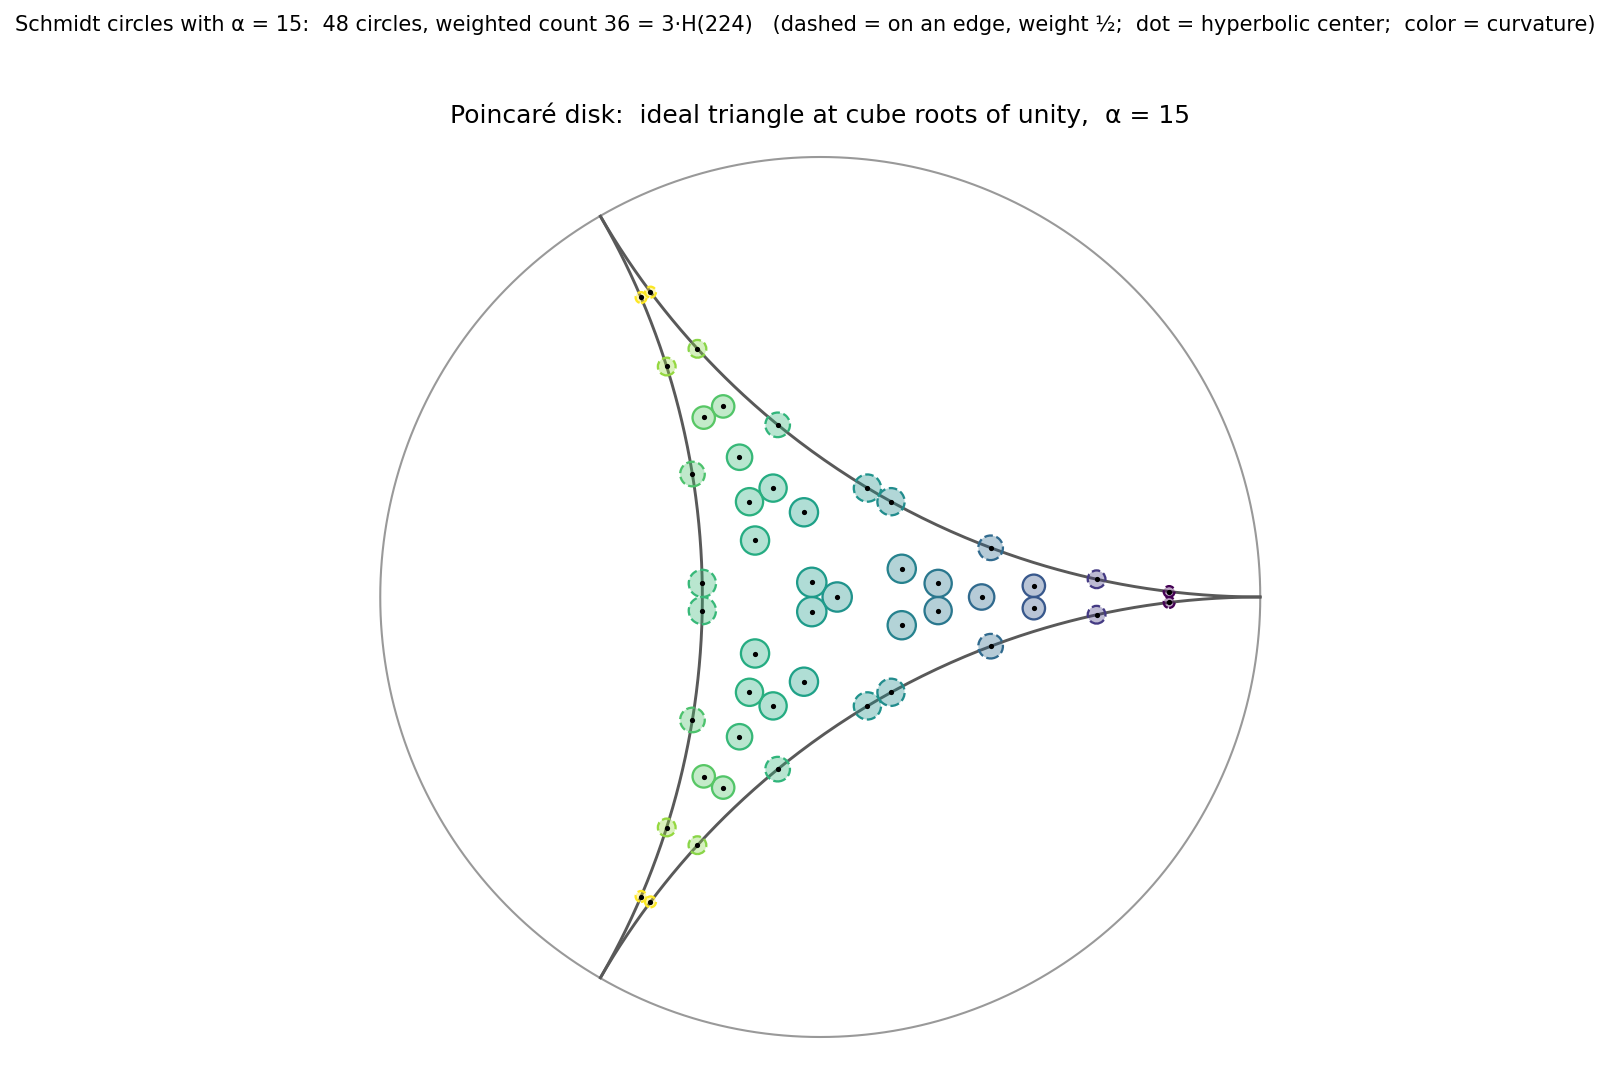
\includegraphics[width=0.6\textwidth]{alpha15-disk.png}
\caption{The $48$ level-$15$ Schmidt circles with hyperbolic center in
the ideal triangle $T = (0, 1, \infty)$, transported to the Poincar\'e
disk, where the order-$3$ symmetry $z \mapsto 1/(1-z)$ of $T$ becomes
exact threefold symmetry (the full symmetry is dihedral).  Weighted
count: $36 = 3H(224)$.  Produced by \texttt{alpha\_circles.py}.}
\label{fig:alpha15}
\end{figure}

Machine verification: \texttt{alpha\_circles.py} implements the level
algorithm (solve $x^2 \equiv 1 - n^2 \bmod 4q$ across $q$), draws the
configurations (Figure \ref{fig:alpha15}), and confirms the weighted
count $= 3H(n^2 - 1)$ for all $2 \le n \le 40$ and spot checks at
$n = 301$ and $n = 1000$.

\subsection{The spherical census: $4H(4(\ell^2 + 1))$}
\label{subsec:sph-count}

Project $\Chat$ stereographically onto the sphere of diameter $1$
tangent to $\C$ at the origin (north pole $(0, 0, 1)$).  On the sphere,
lines are circles too, and compactness makes the census global: no
fundamental domain is needed.

\begin{proposition}[spherical radius]\label{prop:sphradius}
Let $\omega$ be a Schmidt circle with Hermitian data
$M = \begin{pmatrix} 2q & -\zeta \\ -\bar\zeta & 2m \end{pmatrix}$,
$\det M = -1$.  Its stereographic image is a circle of angular radius
$\theta$ (the angle subtended at the sphere's center) with
\[
  \cot\theta \;=\; q + m \;=:\; \ell,
\]
half the sum of curvature and co-curvature --- an integer for every
Schmidt circle.  The lines $\im z = k$ have $\ell = |k|$; the real line
itself is the single great circle ($\ell = 0$).
\end{proposition}

\begin{proof}
A point $(x_0, y_0, t)$ of the sphere satisfies
$x_0^2 + y_0^2 + t^2 = t$ and is the image of $z = (x_0 + iy_0)/(1-t)$.
Substituting into $2q|z|^2 - \zeta\bar z - \bar\zeta z + 2m = 0$ and
clearing $(1 - t)$ shows the image lies in the plane
$x x_0 + y y_0 + (m - q)t = m$ (with $\zeta = x + iy$).  Its distance to
the center $(0, 0, \tfrac12)$ is
$\tfrac{|m + q|}{2}\bigl(|\zeta|^2 + (m - q)^2\bigr)^{-1/2}$, and
$|\zeta|^2 + (m - q)^2 = 4qm + 1 + (m - q)^2 = 1 + (m + q)^2$; dividing
by the radius $\tfrac12$ gives
$\cos\theta = |q + m|/\sqrt{1 + (q + m)^2}$.
\end{proof}

Determinant $-1$ forces $qm \ge 0$, so after orientation $q, m \ge 0$
and $\ell \ge 0$: \emph{the spherical radii of Schmidt circles quantize
to the integer-cotangent angles} $\theta_\ell = \arccot\ell$, and no
other radius occurs.  We call $\ell$ the \emph{spherical level}.

\begin{theorem}[spherical census]\label{thm:spherical}
For $\ell \ge 1$, the number of Schmidt circles of spherical radius
$\arccot\ell$ on the Riemann sphere is
\[
  N_{\mathrm{sph}}(\ell) \;=\; \tfrac13\,r_3(\ell^2 + 1)
  \;=\; 4\,H\bigl(4(\ell^2 + 1)\bigr),
\]
where $r_3(n)$ is the number of representations of $n$ as a sum of three
squares.  Moreover, the finite group
$\Gamma_{\mathrm{sph}} = \SU(2) \cap \SL_2(\Zi)$ --- in $\PSL_2$ the
Klein four-group $\{z, -z, 1/z, -1/z\}$ of rotations by $\pi$ about the
coordinate axes --- acts freely on the level-$\ell$ circles, so the count
on the quotient is exactly $H(4(\ell^2 + 1))$.
\end{theorem}

\begin{proof}
By Theorem \ref{thm:classification}, level-$\ell$ circles are the data
$(q, m, \zeta)$ with $q + m = \ell$, $q, m \ge 0$, $\zeta = x + iy$, $x$
even, $y$ odd, $x^2 + y^2 = 4qm + 1$; the case $q = 0$ gives the lines
$\im z = \pm\ell$, and every admissible datum occurs.  Substituting
$t := q - m$ (so $t \equiv \ell \bmod 2$) turns the constraint into
\[
  x^2 + y^2 + t^2 = \ell^2 + 1, \qquad
  x \equiv 0,\ y \equiv 1,\ t \equiv \ell \pmod 2,
\]
a bijection ($y$ odd excludes $x = y = 0$, so $|t| \le \ell$ is
automatic).  For $\ell$ even, $\ell^2 + 1 \equiv 1 \pmod 4$: every
representation has exactly one odd coordinate, and permuting coordinates
shows the three positions of the odd coordinate are equinumerous; our
parity pattern selects one third.  For $\ell$ odd,
$\ell^2 + 1 \equiv 2 \pmod 4$: exactly two odd coordinates, and the same
argument applies to the position of the even one.  Hence
$N_{\mathrm{sph}}(\ell) = r_3(\ell^2 + 1)/3$.  Since
$\ell^2 + 1 \equiv 1, 2 \pmod 4$ (never $\equiv 0, 4, 7 \bmod 8$),
Gauss's theorem $r_3(n) = 12H(4n)$ applies
\cite[\S4]{Grosswald1985}.  Freeness: the generators act by
$(q, m, \zeta) \mapsto (q, m, -\zeta)$, $(m, q, \bar\zeta)$,
$(m, q, -\bar\zeta)$; a fixed point would force $\zeta$ real
(impossible: $y$ odd) or $\zeta = yi$, $q = m$ with $y^2 = \ell^2 + 1$
(impossible for $\ell \ge 1$).
\end{proof}

\begin{remark}
The antipodal map $z \mapsto -1/\bar z$ preserves the arrangement and
pairs the level-$\ell$ circles freely.  The three slices meet in exactly
one point: $n^2 - 1 = 4(\ell^2 + 1)$ forces $(n, \ell) = (3, 1)$ ---
the discriminant $-8$ is seen twice by the arrangement, once
hyperbolically at level $3$ and once spherically at the $45^\circ$
circles $\ell = 1$.
\end{remark}

Machine verification: \texttt{spherical\_moduli\_invariants.py}
(experiment A) verifies the census by exact enumeration for all
$\ell \le 20$ and the radius formula against fitted circumcircles of
projected points to $40+$ digits.

\subsection{The triptych}

\begin{theorem}[one arrangement, three geometries, three class-number
counts]\label{thm:triptych}
The Gaussian Schmidt arrangement, graded by the natural radius invariant
of each background geometry of $\Chat$, is counted by class numbers in
all three:
\begin{center}
\small
\begin{tabular}{@{}llll@{}}
\toprule
geometry & radius invariant & census & CM data of a level\\
\midrule
Euclidean plane & curvature $2n$ & $N_e(n) = 2h(-4n^2)$ &
conductor $n$ over $\Q(i)$\\
hyperbolic plane & $\coth\rho = n$ & $3H(n^2 - 1)$ &
discriminant $1 - n^2$\\
sphere & $\cot\theta = \ell$ & $4H(4(\ell^2 + 1))$ &
discriminant $-4(\ell^2 + 1)$\\
\bottomrule
\end{tabular}
\end{center}
The Euclidean count is per unit area (Proposition \ref{prop:Ne},
Theorem \ref{thm:euclidstructure}), the hyperbolic count is the weighted
census of an ideal triangle (Theorem \ref{thm:hyperbolic}), and the
spherical count is global (Theorem \ref{thm:spherical}).
\end{theorem}

The three censuses read the coefficients of the classical weight-$3/2$
class-number generating functions \cite{Cohen1975, Zagier1975} along
three quadratic progressions: $d = 4n^2$ (even squares), $d = n^2 - 1$
(shifted squares), $d = 4\ell^2 + 4$.  The corresponding statements for
Zagier's traces of singular moduli \cite{Zagier2002} appear below as
Proposition \ref{prop:traces} and its analogues.

%%% ============================================================
\section{The involution and the class formula}\label{sec:involution}

\subsection{What $\sigma(X) = \bar X^{-1}$ is}\label{subsec:sigma}

Consider
\[
  \sigma: \SL_2(\Zi) \to \SL_2(\Zi), \qquad \sigma(X) = \bar X^{-1}
\]
(entrywise conjugation followed by inversion), an anti-automorphism of
order two.  Throughout, $J = \begin{pmatrix} 0 & 1 \\ -1 &
0\end{pmatrix}$, so $M_0 = iJ$, and for $X \in \SL_2$ one has
$X^{-1} = J^{-1}X^{\mathsf T}J$.

\begin{proposition}\label{prop:unitaryinv}
$\sigma(X) = J^{-1}X^{\dagger}J = M_0^{-1}X^{\dagger}M_0$.  Thus
$\sigma$ is the adjoint anti-involution of the Hermitian form
$h(u, v) = u^{\dagger}M_0 v$ attached to the real line
($h(Xu, v) = h(u, \sigma(X)v)$): in the language of central simple
algebras, a \emph{unitary involution} --- an involution of the second
kind --- on $M_2(\Q(i))$, restricting to Galois conjugation on the
center.  Moreover
\[
  \SU(M_0;\, \Zi) \;=\; \SL_2(\Z):
\]
the unitary group of $h$ over $\Zi$, the stabilizer of the oriented real
line, and the fixed group of the Galois involution
$\theta(X) = \bar X = \sigma(X)^{-1}$ all coincide with
$\Gamma := \SL_2(\Z)$.
\end{proposition}

\begin{proof}
The identity is immediate from $X^{-1} = J^{-1}X^{\mathsf T}J$ and
$\bar X^{\mathsf T} = X^\dagger$.  For the unitary group:
$g^{\dagger}Jg = J$ together with $g^{\mathsf T}Jg = J$ (automatic for
$\det g = 1$) forces $\bar g = g$.
\end{proof}

Circles of the Schmidt arrangement correspond to cosets $X\Gamma$, and
$\Gamma$-classes of circles to double cosets $\Gamma X\Gamma$;
$(\SL_2(\C), \SL_2(\R))$ is the symmetric pair of the real structure
$\theta$, and $\sigma$ is the Gelfand-trick anti-involution of that
pair.  Arithmetically it is far from trivial, as we now see.

\begin{theorem}[Cartan embedding $=$ circle inversion]\label{thm:cartan}
For $X \in \SL_2(\Zi)$ write $M_X$ for the Hermitian matrix of
$X(\Rhat)$ as in \eqref{eq:equivariance}.  Then
\begin{equation}\label{eq:funfact}
  X\bar X^{-1} \;=\; -\,i\,J\,\overline{M_X}
  \;=\; \begin{pmatrix} -iB & -iC \\ iA & i\bar B\end{pmatrix},
  \qquad
  M_X = \begin{pmatrix} A & B \\ \bar B & C \end{pmatrix}.
\end{equation}
Consequently:
\begin{enumerate}
\item the Cartan image $Y = X\bar X^{-1}$ determines and is determined
by the oriented circle $X(\Rhat)$; its fibers are the cosets
$X\,\SL_2(\Z)$;
\item $v \mapsto Y\bar v$ is the anti-holomorphic inversion in the
circle $X(\Rhat)$, and $Y\bar Y = I$ (the Cartan image consists of
twisted involutions);
\item $\tr(X\bar X^{-1}) = -2\,\alpha_{\pm}(X(\Rhat))$, the level with
a sign recording orientation;
\item for a level-$n$ circle, the normalized product of the reflections
of $\HH^3$ in the hemispheres over $X(\Rhat)$ and over $\Rhat$ is a
hyperbolic translation of length $2\arccosh n$ along their common
perpendicular, with characteristic polynomial
$\lambda^2 + 2n\lambda + 1$; every level-$n$ Schmidt circle thus
determines a closed geodesic of length $2\arccosh n$ in the Bianchi
orbifold $\PSL_2(\Zi)\backslash\HH^3$, with real quadratic trace field
$\Q(\sqrt{n^2 - 1})$.
\end{enumerate}
\end{theorem}

\begin{proof}
\eqref{eq:funfact} is a direct computation from \eqref{eq:image}
applied to $X^{-1}$, using $\bar X^{-1} = J^{-1}X^{\dagger}J$.  (1) The
right side of \eqref{eq:funfact} is a bijective affine function of
$M_X$; and $M_{X\gamma} = M_X$ for $\gamma \in \SL_2(\Z)$ while
conversely $Y(X') = Y(X)$ forces $X^{-1}X' \in \SL_2(\R) \cap \SL_2(\Zi)
= \SL_2(\Z)$.  (2) Rescaling $Y$ by $1/(iA)$ puts it in the classical
form $\begin{pmatrix} z_0 & r^2 - |z_0|^2 \\ 1 & -\bar
z_0\end{pmatrix}$ of the inversion in the circle of center $z_0$,
radius $r$; conceptually, $\Rhat$ is the fixed locus of $z \mapsto \bar
z$, so $X(\Rhat)$ is the fixed locus of
$X \circ \mathrm{conj} \circ X^{-1}$, whose M\"obius part is $Y$.
(3) $\tr Y = -iB + i\bar B = 2\im B = -2y$ with $y$ the oriented height
numerator, which is $\alpha_\pm$ by Proposition \ref{prop:level}.
(4) The composite of the two inversions is the M\"obius transformation
$-Y$-normalized, an isometry of $\HH^3$ with characteristic polynomial
$\lambda^2 + 2n\lambda + 1$ and eigenvalue $-(n + \sqrt{n^2 - 1})$;
its translation length is $2\log(n + \sqrt{n^2 - 1}) = 2\arccosh n$.
Both reflecting planes are $\PSL_2(\Zi)$-hemispheres, so the composite
lies in $\PSL_2(\Zi)$ and its axis projects to a closed geodesic.
\end{proof}

\begin{remark}
Statement (4) is the three-dimensional, $\sigma$-twisted analogue of
the trace-$t$ conjugacy classes underlying reciprocal geodesics on the
modular surface \cite{Sarnak2007}: the length spectrum value
$2\arccosh n$ arises here with multiplicity governed by
$H(n^2 - 1)$-data, through the fibers of the circle-to-geodesic map
described in Corollary \ref{cor:geodesicfibers} below.  We know of no
prior appearance of this correspondence.
\end{remark}

\subsection{Fixed points: exactly three twisted classes}

By Proposition \ref{prop:unitaryinv} one has $\sigma(X) = X$ iff
$M_0X$ is Hermitian, iff $X = M_0M$ with $M$ integral Hermitian of
determinant $-1$: \emph{the fixed points of $\sigma$ are precisely the
matrices of circle inversions} $z \mapsto M_0M(\bar z)$, one for each
integral Hermitian form of determinant $-1$.  The natural action
preserving the fixed set is the twisted conjugation
$X \mapsto \bar g X g^{-1}$, matching the action
\eqref{eq:equivariance} on forms; classifying fixed points up to
twisted conjugacy is a Galois-cohomology problem (over the field,
Hilbert 90 trivializes it; over $\Zi$ it is a genus question).

\begin{proposition}[computational]\label{prop:threeclasses}
Among the integral binary Hermitian forms of determinant $-1$ with
$|A|, |C| \le 20$, there are exactly three
$\SL_2(\Zi)$-classes:
\begin{enumerate}
\item the class of $M_0$: the Schmidt arrangement $\Sarr$
($B \equiv i \bmod 2$; horizontal lines, even curvatures);
\item the class of $\begin{pmatrix} 0 & 1 \\ 1 & 0 \end{pmatrix}$: the
rotated family $i\Sarr$ ($B \equiv 1 \bmod 2$; vertical lines);
\item the class of $\operatorname{diag}(1, -1)$ (the unit circle): all
circles of \emph{odd} curvature --- a family that is not part of the
Schmidt arrangement at all.
\end{enumerate}
The three classes are pairwise distinct for all forms (the diagonal and
off-diagonal parities mod $2$ are invariants); the completeness of the
list is verified by exhaustive orbit enumeration within the stated
bounds by the script \texttt{involution\_\allowbreak experiments.py}.  Orientation-reversed
seeds land in the same three classes.
\end{proposition}

Thus ``the Schmidt arrangement'' is one twisted Galois class of real
structures on $\mathbb{P}^1$; the involution $\sigma$ is the algebraic
shadow of this descent picture.

\subsection{The class formula}\label{subsec:classformula}

$\sigma$ maps $\Gamma X\Gamma \mapsto \Gamma\sigma(X)\Gamma$ (well
defined since $\sigma(\Gamma) = \Gamma$), hence induces an involution
$\hat\sigma$ on $\Gamma$-classes of oriented Schmidt circles, i.e.\ ---
via Proposition \ref{prop:formdictionary}, at odd level $n$ --- on form
classes of discriminant $D = 1 - n^2$.  Composition with the reflection
$z \mapsto \bar z$ (which returns images to the upper half-plane and
preserves each form class) makes $\hat\sigma$ an involution of the
class set.  Here is what it is.

\begin{theorem}[class formula]\label{thm:classformula}
Let $n \ge 3$ be odd, $D = 1 - n^2$, and let $f$ be a primitive
positive definite form of discriminant $D$, with $X \in \SL_2(\Zi)$ any
matrix whose circle $X(\Rhat)$ lies in the $\SL_2(\Z)$-class of $f$.
Then the circle of $\sigma(X)$ lies in the lower half-plane with
reversed orientation and level $-n$, and its reflection into the upper
half-plane lies in the class
\[
  \hat\sigma[f] \;=\; [\idealr_n]\,[f]^{-1},
  \qquad
  \idealr_n = \Bigl[\Bigl(\tfrac{n-1}{2},\,0,\,\tfrac{n+1}{2}\Bigr)\Bigr],
\]
product and inverse taken in the form class group of discriminant $D$.
\end{theorem}

The twist is a canonical \emph{ambiguous} ($2$-torsion) class: as an
ideal, $\idealr = \bigl(\tfrac{n-1}{2}, \omega\bigr)$ with
$\omega = \sqrt{D}/2$, and $\idealr^2 = \bigl(\tfrac{n-1}{2}\bigr)$,
while $\ideals = \bigl(\tfrac{n+1}{2}, \omega\bigr)$ satisfies
$[\ideals] = [\idealr]$ and $\idealr\ideals = (\omega)$.  Since
$[f]^{-1} = [\bar\ideala]$ for the ideal class $[\ideala]$ of $f$, the
theorem reads
\[
  \hat\sigma: [\ideala] \longmapsto [\idealr_n\,\bar\ideala]:
\]
Galois conjugation of the class group twisted by a distinguished
ambiguous class --- formally identical to the Atkin--Lehner action
$w_N : [\ideala] \mapsto [\mathfrak{n}\bar\ideala]$ on Heegner points,
with $\idealr_n$ in the role of $\mathfrak{n}$.  Geometrically,
$\idealr_n$ is the class of the circles tangent to the lines of the
arrangement: its representative circle has curvature $n - 1$, center
$\tfrac{ni}{n-1}$, and touches $\im z = 1$.

The proof occupies the rest of this subsection.  We use the ideal
dictionary in the following normalization (Gauss; see
\cite[\S7]{Cox2013}): $K = \Q(\sqrt D)$ with $\sqrt D := i\sqrt{n^2 -
1}$, $\omega = \sqrt D/2$, $\mathcal{O} = \Z[\omega]$ the order of
discriminant $D$; for a proper $\mathcal{O}$-ideal $\idealb$ with
$\Z$-basis $(\alpha, \beta)$, the basis is \emph{positively oriented}
if $\im(\bar\alpha\beta) > 0$, and
$f_{\idealb}(s, t) = N(s\alpha + t\beta)/N(\idealb)$; then $[\idealb]
\mapsto [f_\idealb]$ is an isomorphism onto the primitive form class
group, a negatively oriented basis producing the inverse class;
$\ideala_f := \Z a + \Z(\tfrac b2 + \omega)$ satisfies
$f_{\ideala_f} = f$; and $\ideals = \Z\tfrac{n+1}{2} + \Z\omega$ has
$f_{\ideals} = \bigl(\tfrac{n+1}{2}, 0, \tfrac{n-1}{2}\bigr)$, so
$[\ideals] = \idealr_n$, with $\bar\ideals = \ideals$, confirming that
$\idealr_n$ is $2$-torsion (as it must be for $\hat\sigma$ to be an
involution).  A form $f = (a, b, c)$ of discriminant $D$ ($b$
automatically even) corresponds to the circle
\[
  M_f = \begin{pmatrix} 2a & b - ni \\ b + ni & 2c\end{pmatrix}
  \qquad (\text{curvature } 2a, \ \text{center } \tfrac{-b + ni}{2a}).
\]
Since $\hat\sigma$ is defined on double cosets, it suffices to prove
the theorem for one $X$ per class; we construct one in closed form.

\begin{lemma}[explicit unitary basis; the closed-form section]
\label{lem:lemmaA}
Let $f = (a, b, c)$ have discriminant $D = 1 - n^2$, and let
\[
  \mathcal{K} := \bigl\{(s, t) \in \Z^2 \;:\;
  (n+1)s \equiv bt, \quad bs \equiv -(n-1)t \pmod{2a}\bigr\}.
\]
Then $\mathcal{K}$ has index $a$ in $\Z^2$.  For any basis
$w_1 = (s_1, t_1)$, $w_2 = (s_2, t_2)$ of $\mathcal{K}$ with
$t_1s_2 - s_1t_2 = a$, put $u_k = s_k + it_k$ and
\[
  v_k \;=\; \frac{(n + bi)\,u_k + \bar u_k}{2ia} \qquad (k = 1, 2).
\]
Then
\[
  P = \begin{pmatrix} u_1 & v_1 \\ u_2 & v_2 \end{pmatrix}
  \in \SL_2(\Zi)
  \qquad\text{and}\qquad
  P^{\dagger} M_0 P = M_f;
\]
equivalently, $X := P^{-1}$ satisfies $X(\Rhat) = $ the circle $M_f$.
\end{lemma}

\begin{proof}
\emph{Index.}  $\mathcal{K} = \ker(R \bmod 2a)$ for
$R = \begin{pmatrix} n+1 & -b \\ b & n-1\end{pmatrix}$,
$\det R = n^2 - 1 + b^2 = 4ac$.  All entries of $R$ are even and
$\gcd(\tfrac{n+1}{2}, \tfrac{n-1}{2}) = 1$, so the Smith invariants of
$R$ are $(2, 2ac)$; hence
$\#\ker(R \bmod 2a) = \gcd(2, 2a)\gcd(2ac, 2a) = 4a$ and
$[\Z^2 : \mathcal{K}] = (2a)^2/4a = a$.

\emph{Integrality of $v_k$.}
$(n + bi)(s + it) + (s - it) = [(n+1)s - bt] + i[bs + (n-1)t]$, so
$2ia \mid (n + bi)u_k + \bar u_k$ iff $(s_k, t_k) \in \mathcal{K}$.

\emph{Gram identities.}  Write $z := u_1\bar u_2$, so
$\im z = t_1s_2 - s_1t_2 = a$.  Then $h(p_1, p_1) = 2\im(u_1\bar u_2)
= 2a$;
$\det P = (u_1\bar u_2 - u_2\bar u_1)/(2ia) = 1$;
$\bar u_1v_2 - \bar u_2v_1 = (n + bi)(\bar u_1u_2 - \bar
u_2u_1)/(2ia) = -(n + bi)$, giving $h(p_1, p_2) = b - ni$; and in
$v_1\bar v_2$ the cross terms are conjugate, hence real, so
\[
  \im(v_1\bar v_2)
  = \frac{(n^2 + b^2)\im z + \im\bar z}{4a^2}
  = \frac{(n^2 + b^2 - 1)a}{4a^2} = \frac{4ac}{4a} = c,
\]
i.e.\ $h(p_2, p_2) = 2c$.  (Here $p_1, p_2$ denote the columns of
$P$ and $h$ the form of Proposition \ref{prop:unitaryinv}.)
\end{proof}

For example $n = 3$, $f = (1, 0, 2)$: $\mathcal{K} = \Z^2$, and
$w_1 = (0, 1)$, $w_2 = (1, 0)$ give
$P = \begin{pmatrix} i & 1 \\ 1 & -2i\end{pmatrix}$.  Lemma
\ref{lem:lemmaA} is of independent computational value: it writes down,
in closed form, an element of $\SL_2(\Zi)$ realizing any prescribed
Schmidt circle --- previously available only through the descent
algorithm of Theorem \ref{thm:classification}.  It is the engine of
most verification scripts in this paper, and of the phase computations
of Section \ref{sec:phase}.

\begin{lemma}[the Gram matrix of the $\sigma$-image]\label{lem:lemmaB}
Let $X = P^{-1}$, so $\sigma(X) = \bar P$, and let
$N = (P^{-1})^{\dagger}M_0P^{-1}$, so that the image circle is
$M_{\sigma X} = -\bar N$.  With
$g(s, t) := (n+1)s^2 + (n-1)t^2$ and polarization
$g(w, w') = (n+1)ss' + (n-1)tt'$:
\[
  N = \begin{pmatrix}
  \dfrac{g(w_2)}{a} & -\dfrac{g(w_1, w_2)}{a} - ni \\[2mm]
  -\dfrac{g(w_1, w_2)}{a} + ni & \dfrac{g(w_1)}{a}
  \end{pmatrix},
\]
and all displayed rational numbers are integers, the diagonal ones
even.
\end{lemma}

\begin{proof}
The columns of $P^{-1}$ are $(v_2, -u_2)^{\mathsf T}$ and
$(-v_1, u_1)^{\mathsf T}$.  Using $\tfrac{1}{2ia} = \tfrac{-i}{2a}$:
\[
  N_{11} = -2\im(v_2\bar u_2)
  = \frac{\re[(n + bi)|u_2|^2 + \bar u_2^{\,2}]}{a}
  = \frac{n|u_2|^2 + \re(u_2^2)}{a} = \frac{g(w_2)}{a},
\]
symmetrically $N_{22} = g(w_1)/a$, and
$N_{12} = i(u_1\bar v_2 - \bar u_2 v_1) = -g(w_1, w_2)/a - ni$ by the
same expansion with $u_1\bar u_2 = (s_1s_2 + t_1t_2) + ia$.
\emph{Integrality:} multiplying the two congruences defining
$\mathcal{K}$ by $s$ resp.\ $t$ gives
$(n+1)s^2 \equiv bst$ and $(n-1)t^2 \equiv -bst \pmod{2a}$, so
$g(w) \equiv 0 \pmod{2a}$ on $\mathcal{K}$; polarizing,
$2g(w_1, w_2) = g(w_1 + w_2) - g(w_1) - g(w_2) \equiv 0 \pmod{2a}$.
\end{proof}

Two consequences are immediate.  The oriented image $M_{\sigma X} =
-\bar N$ has curvature entry $-g(w_2)/a < 0$: $\hat\sigma$
\emph{always reverses orientation}.  The unoriented image lies in the
lower half-plane with $|y| = n$: $\alpha$ \emph{is preserved}.
Reflecting by $z \mapsto \bar z$, the image form, read in the basis
$(w_2, -w_1)$ of $\mathcal{K}$ (same orientation as $(w_1, w_2)$), is
\begin{equation}\label{eq:fprime}
  f' := \Bigl(\frac{g(w_2)}{2a},\ -\frac{g(w_1, w_2)}{a},\
  \frac{g(w_1)}{2a}\Bigr) = \frac{1}{2a}\,g\big|_{\mathcal{K}},
\end{equation}
of discriminant $\disc(g)\cdot a^2/(2a)^2 = D$.  \emph{So the image
class is the $\idealr_n$-form $\tfrac12 g = (\tfrac{n+1}{2}, 0,
\tfrac{n-1}{2})$, restricted to the index-$a$ lattice $\mathcal{K}$ and
divided by $a$.}  It remains to recognize this as composition.

\begin{lemma}[$\mathcal{K}$ is an ideal, and it factors]
\label{lem:lemmaC}
Embed $\iota: \Z^2 \hookrightarrow K$,
$\iota(s, t) = s\,\tfrac{n+1}{2} + t\,\omega$, so
$\iota(\Z^2) = \ideals$.  Then $\idealc := \iota(\mathcal{K})$ is an
$\mathcal{O}$-ideal, and for $f$ primitive,
$\idealc = \ideals\,\ideala_f$.
\end{lemma}

\begin{proof}
\emph{$\omega$-stability.}  $\omega\,\iota(s, t) =
\iota\bigl(\tfrac{1-n}{2}t,\ \tfrac{n+1}{2}s\bigr)$, and the image pair
satisfies the $\mathcal{K}$-congruences: substituting,
\begin{gather*}
  (n+1)\tfrac{1-n}{2}t - b\tfrac{n+1}{2}s
  = -\tfrac{n+1}{2}\bigl[bs + (n-1)t\bigr],\\
  b\tfrac{1-n}{2}t + (n-1)\tfrac{n+1}{2}s
  = \tfrac{n-1}{2}\bigl[(n+1)s - bt\bigr],
\end{gather*}
both multiples of the defining congruences, hence
$\equiv 0 \pmod{2a}$.

\emph{Containment $\ideals\ideala_f \subseteq \idealc$.}  The four
generators of $\ideals\ideala_f$ have $\iota$-coordinates
$(a, 0)$, $(\tfrac b2, \tfrac{n+1}{2})$, $(0, a)$,
$(\tfrac{1-n}{2}, \tfrac b2)$, and each lies in $\mathcal{K}$: for the
first and third use that $b$ and $n \pm 1$ are even; for the second,
$(n+1)\tfrac b2 - b\tfrac{n+1}{2} = 0$ and $b\tfrac b2 +
(n-1)\tfrac{n+1}{2} = \tfrac{b^2 + n^2 - 1}{2} = 2ac \equiv 0
\pmod{2a}$; for the fourth, $(n+1)\tfrac{1-n}{2} - b\tfrac b2 = -2ac$
and $b\tfrac{1-n}{2} + (n-1)\tfrac b2 = 0$.

\emph{Equality.}  Both sides sit inside $\ideals$ with the same index:
$[\ideals : \idealc] = [\Z^2 : \mathcal{K}] = a$, and --- here
primitivity of $f$ enters --- $\ideala_f$ is proper, so
$[\ideals : \ideals\ideala_f] = N(\ideala_f) = a$.  A containment of
equal finite index is an equality.
\end{proof}

\begin{proof}[Proof of Theorem \ref{thm:classformula}]
By Lemma \ref{lem:lemmaC} and $N \circ \iota = \tfrac{n+1}{2}\cdot
\tfrac12 g$, the form \eqref{eq:fprime} is the norm form of the proper
ideal $\idealc = \ideals\ideala_f$ of norm $\tfrac{n+1}{2}a$, computed
in the basis $(\iota(w_2), \iota(-w_1))$.  This basis is
\emph{negatively} oriented: for $w = (s, t)$, $w' = (s', t')$,
\[
  \im\bigl(\overline{\iota(w)}\,\iota(w')\bigr)
  = \tfrac{n+1}{2}\cdot\tfrac{\sqrt{n^2 - 1}}{2}(st' - ts'),
\]
and for the pair $(w_2, -w_1)$: $s_2(-t_1) - t_2(-s_1) = -a < 0$.  A
negatively oriented basis yields the opposite class, so by the
dictionary,
\[
  [f'] = [f_{\idealc}]^{-1} = \bigl([\ideals][\ideala_f]\bigr)^{-1}
  = [\idealr_n]^{-1}[f]^{-1} = [\idealr_n][f]^{-1},
\]
the last step because $\idealr_n$ is $2$-torsion.
\end{proof}

Note where each ingredient comes from: the \emph{inversion} $[f]^{-1}$
comes from the orientation flip of complex conjugation inside $\sigma$
(the $-a < 0$ computation); the \emph{twist} $\idealr_n$ comes from the
Gram form $g(s, t) = n|u|^2 + \re(u^2)$ --- the norm form twisted by
Galois conjugation $u \mapsto \bar u$, exactly the fingerprint $\sigma$
leaves on the Gram matrix --- whose class is forced to be the split of
$n^2 - 1$ into the two even parts $\tfrac{n\pm1}{2}\cdot 2$.

\begin{corollary}\label{cor:fixedclasses}
$\hat\sigma$ has a fixed class iff $\idealr_n$ is a square in the class
group (iff $\idealr_n$ lies in the principal genus); the fixed classes
then form a coset of the $2$-torsion.  For $n = 11$ (discriminant
$-120$, class group $(\Z/2)^2$, three distinct nontrivial ambiguous
classes --- the decisive test case) there are none: $\hat\sigma$ sends
the principal class to $[(5, 0, 6)] = \idealr_{11}$, not to
$[(2, 0, 15)]$ nor $[(3, 0, 10)]$, and swaps the other two, exactly as
$[\idealr][f]^{-1}$ predicts.  For $n = 9$ (class group $\Z/4$,
$\idealr_9$ the square of a generator) the two order-$4$ classes
$[(3, \pm 2, 7)]$ are fixed.
\end{corollary}

\begin{corollary}[fibers of the circle-to-geodesic map]
\label{cor:geodesicfibers}
$\hat\sigma$ preserves each $\SL_2(\Zi)$-conjugacy class of Cartan
images $Y$; hence the unordered pair $\{[f], [\idealr_n][f]^{-1}\}$ is
an invariant of the closed geodesic of Theorem \ref{thm:cartan}(4)
attached to the circle, and the circle-to-geodesic map identifies
exactly the $\hat\sigma$-orbits of classes.
\end{corollary}

\begin{remark}[imprimitive classes; verified, unproved]
\label{rem:imprimitive}
On the imprimitive classes of content $g$, machine computation
(\texttt{involution\_classmap.py}, all classes of all odd $n \le 41$)
shows that $\hat\sigma$ is likewise $t_0\cdot[f_0]^{-1}$ on the
underlying primitive classes of discriminant $(1 - n^2)/g^2$, where the
twist $t_0$ is an ambiguous class --- in all computed cases the natural
image of $\idealr_n$ with the $g^2$-part of its norm removed (e.g.\
$n = 15$, $g = 2$: $t_0 = [(2, 0, 7)]$).  The only step of the proof
using primitivity is the index count in Lemma \ref{lem:lemmaC}; at the
ramified prime $2$ the ideal $\ideala_f$ is not proper and
$\ideals\ideala_f \subsetneq \idealc$ can occur.  A clean general
statement on these strata remains open; we do not use them anywhere in
this paper.
\end{remark}

Machine verification: every identity of this section is checked in
exact arithmetic --- \texttt{involution\_experiments.py} for
\eqref{eq:funfact} and the fixed-point characterization,
\texttt{involution\_classmap.py} for the class map at every class of
every odd $n \le 41$, and \texttt{proof\_check.py} for every lemma of
the proof (Lemmas \ref{lem:lemmaA}--\ref{lem:lemmaC} and the
conclusion) at all $169$ primitive classes with odd $n \le 41$.

%%% ============================================================
\section{Composition in circle language}\label{sec:composition}

Fix a level $n \ge 2$.  By Proposition \ref{prop:formdictionary} the
$\SL_2(\Z)$-classes of level-$n$ circles carry the group structure of
the form class group $\Cl(1 - n^2)$ (restricting to primitive classes).
This section answers, in elementary terms: \emph{what do the group
operations do to the circles?}  Think of $\omega_{q,x}$ as a fraction:
a denominator $q$ (half the curvature) and a numerator $x$ (horizontal
position in units of $\tfrac1{2q}$), the height locked to the level.
Sliding by $\Gamma = \PSL_2(\Z)$ costs nothing (translations change
$x$ by $2q$), and the \emph{identity class} is that of the top circle:
$q = 1$, radius $\tfrac12$, the largest circles of the level.

\begin{proposition}[inverse $=$ mirror]\label{prop:mirror}
The inverse of a circle class is its mirror image: the reflection
$z \mapsto -\bar z$ sends $\omega_{q,x} \mapsto \omega_{q,-x}$, i.e.\
$f = (q, -x, m) \mapsto (q, x, m)$, the opposite form.  Inversion in
the unit circle sends $\omega_{q,x}$ to $\omega_{m,x}$ (curvature and
co-curvature trade places), again the inverse class.  In general,
\emph{every orientation-reversing symmetry of the Schmidt arrangement
inverts every class}, being an improper equivalence of forms.
\end{proposition}

\begin{corollary}[$2$-torsion $=$ mirror symmetry]\label{cor:2torsion}
A circle class equals its own inverse iff some
$\Gamma$-translate of the circle has its hyperbolic center on a mirror
line of the modular tessellation.  The three reduced shapes of
ambiguous forms match the three basic mirrors:
\begin{center}
\begin{tabular}{@{}lll@{}}
\toprule
reduced form & circle & mirror \\
\midrule
$b = 0$ & $x = 0$: hyperbolic center on $\re z = 0$ & vertical line \\
$b = a$ & $x = q$: center on $\re z = \tfrac12$ & half-integer
vertical \\
$a = c$ & $q = m$: center on $|z| = 1$ & unit semicircle \\
\bottomrule
\end{tabular}
\end{center}
(For $q = m$: $|z_{\mathrm{hyp}}|^2 = m/q$.)  This makes the all-edge
phenomenon of Section \ref{subsec:hyp-count} transparent: at
$n = 3, 5$ every class is ambiguous, so every circle of the ideal
triangle sits on a mirror --- and the triangle's edges are mirrors.
\end{corollary}

\begin{theorem}[composition $=$ CRT $=$ magnification]
\label{thm:composition}
To compose classes of $\omega_1 = \omega_{q_1, x_1}$ and
$\omega_2 = \omega_{q_2, x_2}$ at level $n$:
\begin{enumerate}
\item slide the circles within their classes until $q_1, q_2$ are
coprime (always possible: the half-curvatures occurring in a class are
exactly the integers primitively represented by its form);
\item the composed class is that of the unique level-$n$ circle with
half-curvature $q_1q_2$ whose numerator satisfies
\[
  x_3 \equiv x_1 \pmod{2q_1}, \qquad x_3 \equiv x_2 \pmod{2q_2}.
\]
\end{enumerate}
Equivalently, geometrically: $\omega_1 * \omega_2$ is the unique
arrangement circle of curvature $2q_1q_2$ that \emph{magnifies onto its
factors}: $q_2\cdot(\omega_1 * \omega_2)$ is a translate of $\omega_1$
and $q_1\cdot(\omega_1 * \omega_2)$ is a translate of $\omega_2$.  This
is Gauss composition.
\end{theorem}

\begin{proof}
Existence and uniqueness are CRT: the moduli $2q_1, 2q_2$ have gcd
$2$ and $x_1 \equiv x_2 \pmod 2$ (both determined by the parity of
$n$), so $x_3$ exists, unique mod $2q_1q_2$; the congruence
$x_3^2 \equiv 1 - n^2 \pmod{4q_1q_2}$ follows from the two factors by
CRT.  The magnification formulation is one line: $x_3 \equiv x_1
\pmod{2q_1}$ says the $q_2$-fold magnification of $\omega_3$ (radius
$\tfrac{1}{2q_1}$, center $\tfrac{x_3 + ni}{2q_1}$) differs from
$\omega_1$ by the integer translation $\tfrac{x_3 - x_1}{2q_1}$.  (An
integer magnification $z \mapsto kz$ with $k \mid q$ sends
$\omega_{q,x}$ to a level-$n$ arrangement circle of half-curvature
$q/k$; for $k \nmid q$ the image leaves the arrangement.)  That the
recipe is Gauss composition: in ideal language the circle
$\omega_{q,x}$ corresponds to $\ideala = \Z q + \Z\theta$,
$\theta = \tfrac{-x + \sqrt D}{2}$, and for coprime $q_1, q_2$ and the
CRT numerator $x_3$,
\[
  (q_1, \theta_3)(q_2, \theta_3)
  = (q_1q_2,\ q_1\theta_3,\ q_2\theta_3,\ \theta_3^2)
  = (q_1q_2, \theta_3),
\]
since coprimality puts $\theta_3$ in the product and
$\theta_3^2 = -x_3\theta_3 - N(\theta_3)$ with
$q_1q_2 \mid N(\theta_3)$.  This is multiplication of ideals ---
equivalently Dirichlet composition of the concordant forms
$(q_1, -x_3, q_2m_3)$ and $(q_2, -x_3, q_1m_3)$ \cite[\S3]{Cox2013}.
\end{proof}

\begin{example}[level $9$; $D = -80$, class group $\Z/4$]
Compose $\omega_{3,4}$ (class $(3, 2, 7)$, a generator) with
$\omega_{4,0}$ (class $(4, 0, 5)$): CRT gives $x_3 \equiv 4\ (6)$,
$\equiv 0\ (8)$, so $x_3 = 16$ and the composite is $\omega_{12, 16}$;
indeed $4\,\omega_{12,16}$ has center $\tfrac{16 + 9i}{6}$, a translate
of $\omega_{3,4}$, and in classes $[(3,2,7)]\cdot[(4,0,5)] =
[(3,-2,7)]$.  Squaring $\omega_{3,4}$: the factors share $q = 3$, so
slide one copy --- $(3, 2, 7)$ also represents $7$, giving
$\omega_{7,2}$ --- then $x_3 \equiv 4\ (6)$, $\equiv 2\ (14)$ gives
$x_3 = 16$, composite $\omega_{21,16}$, whose form $(21, -16, 4)$
reduces to $(4, 0, 5)$: the order-$2$ class, as it must be.
\end{example}

\begin{figure}
\centering
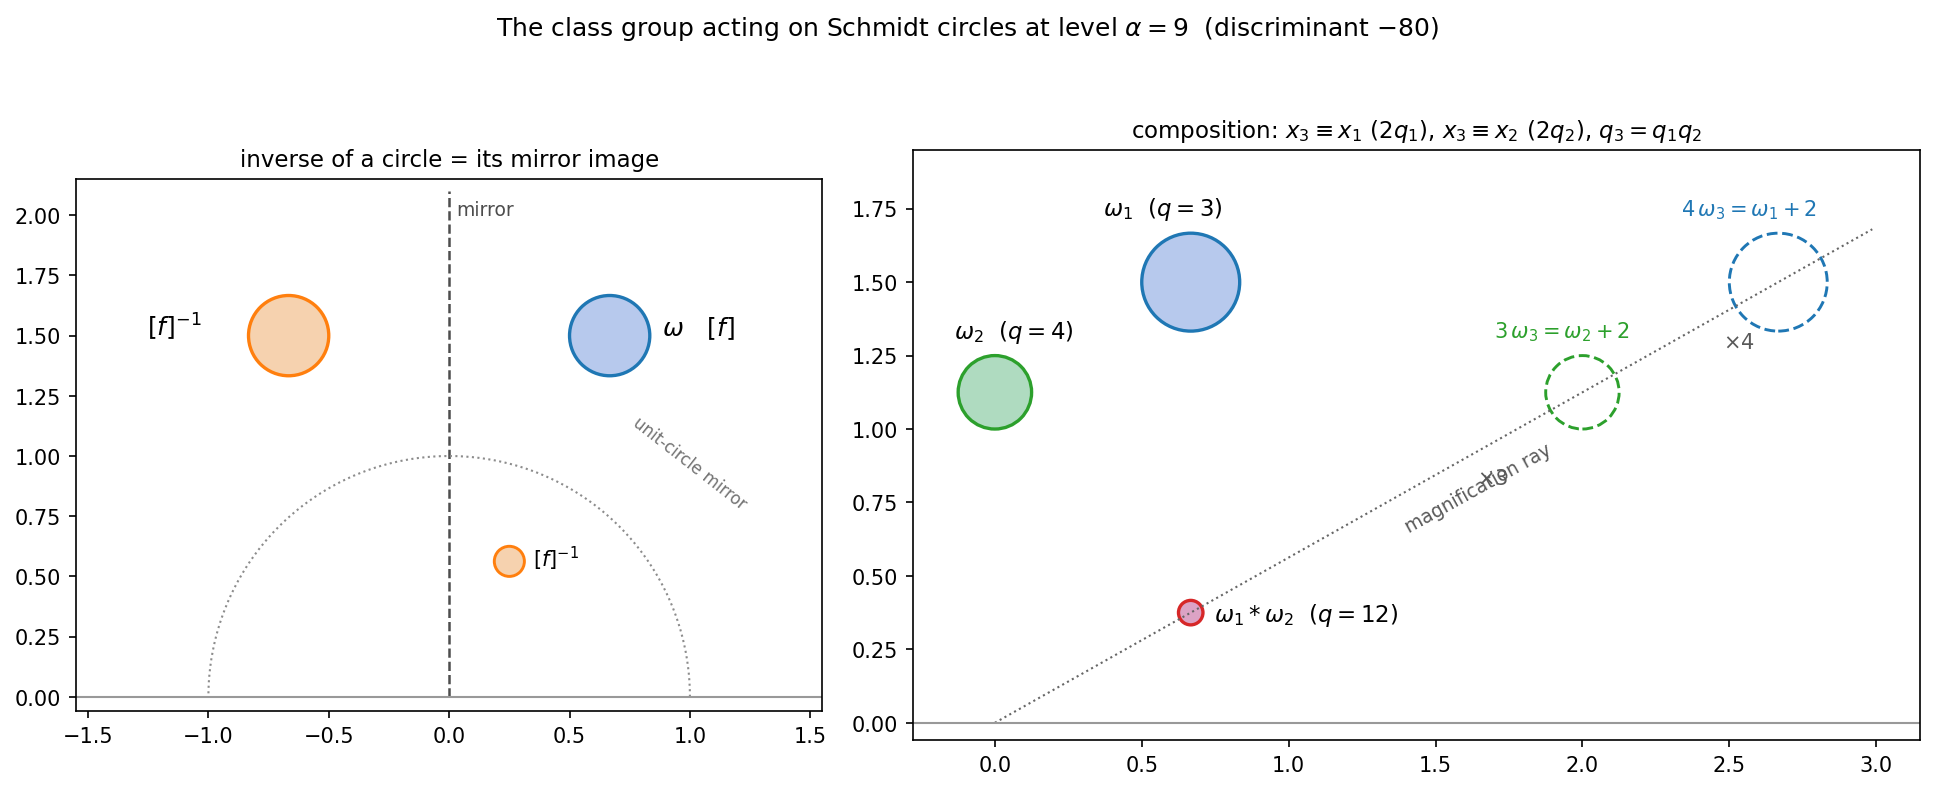
\includegraphics[width=0.8\textwidth]{composition-n9.png}
\caption{Inverse $=$ mirror and composition $=$ magnification at level
$n = 9$.  The three centers involved in each magnification are
collinear with $0$.  Produced by
\texttt{make\_composition\_figure.py}.}
\label{fig:composition}
\end{figure}

\subsection{Matrix-level composition}\label{subsec:matrixcomp}

Suppose the circles are handed to us as $X(\Rhat)$, $Y(\Rhat)$ with
$X, Y \in \SL_2(\Zi)$.  Three facts calibrate what the matrices buy.

\begin{proposition}\label{prop:WX}
Let $X$ be oriented so that $\tr Z_X = -2n$, $Z_X = X\bar X^{-1}$.
Then
\[
  W_X \;:=\; \tfrac{i}{2}\bigl(Z_X + nI\bigr)
  \;=\; \begin{pmatrix} -x/2 & m \\ -q & x/2 \end{pmatrix}
\]
is an integral matrix whose entries are the circle data of
$X(\Rhat) = \omega_{q,x}$ (curvature $2q$, numerator $x$, co-curvature
$2m$): the form $f_X = (q, -x, m)$ can be read off $X$ by one affine
expression in the Cartan image, with no centers, radii or B\'ezout
completions.  Slides act by conjugation: $Z_{T^kX} = T^kZ_XT^{-k}$.
Moreover $W_X$ is the matrix of multiplication by $\omega = \sqrt D/2$
on the lattice $\Lambda = P\Z^2$ of Lemma \ref{lem:lemmaA}: the
integrality of $W_X$ --- equivalently the Schmidt congruence
$\zeta \equiv i \pmod 2$ --- exhibits $\Lambda$ as a module over the
quadratic order $\mathcal{O} = \Z[W_X]$ of discriminant $1 - n^2$, and
Cayley--Hamilton for $W_X$ re-proves the trace identity
$\tr(X\bar X^{-1}) = \pm 2n$ intrinsically.
\end{proposition}

\begin{proof}
Immediate from \eqref{eq:funfact}: $Z_X = -iJ\bar M_X$ has entries
carrying $A, B, C$, and the displayed affine shift extracts the real
part of the form.  For the module statement: on $\Lambda$ the Hermitian
form decomposes as $h|_\Lambda = 2f - ni\langle\cdot,\cdot\rangle$ with
$\langle\cdot,\cdot\rangle$ the standard symplectic form; writing
$Z = P\bar P^{-1}$, one finds $f(\lambda, \mu) = \langle \lambda,
W\mu\rangle$ with $W = \tfrac i4(Z - Z^{-1})$, and
$Z + Z^{-1} = (\tr Z)I$ turns this into $W = \tfrac i2(Z + nI)$; then
$W^2 = \tfrac{4 - (\tr Z)^2}{16}I$ by Cayley--Hamilton while
determinant bookkeeping forces $W^2 = \tfrac D4 I$, so
$\tr Z = \pm 2n$.
\end{proof}

\begin{proposition}[align and conjugate]
\label{prop:aligncompose}
Assume $\gcd(q_X, q_Y) = 1$.  Slide both matrices, $X \mapsto
T^{k_X}X$, $Y \mapsto T^{k_Y}Y$, so that both numerators equal the CRT
value $x_3$ of Theorem \ref{thm:composition} (the concordant position,
in which the two centers are collinear with $0$).  Then with
$E_k = \operatorname{diag}(k, 1)$,
\[
  W_3 \;=\; E_{q_Y}^{-1}\,W_X\,E_{q_Y} \;=\; E_{q_X}^{-1}\,W_Y\,E_{q_X}:
\]
the two conjugates are equal as matrices, integral, and read off the
composed circle $(q_Xq_Y, x_3)$.  An explicit $X_3 \in \SL_2(\Zi)$ with
this circle is then given in closed form by Lemma \ref{lem:lemmaA}.
\end{proposition}

\begin{proof}
Divisibility of the conjugates is exactly the CRT congruence, and their
equality is the matrix form of ``$\omega_3$ magnifies onto both
factors'': conjugating $W_{\omega_3}$ by $E_{q_Y}$ scales the
anti-diagonal by $q_Y^{\pm1}$, turning the data $(q_Xq_Y, x_3, m_3)$
into $(q_X, x_3, q_Ym_3)$, the concordant representative of
$\omega_1$'s class, and symmetrically.
\end{proof}

\begin{remark}[no universal product formula]\label{rem:noproduct}
A plain matrix product does not compose: the circle of $XY$ is
$X(\omega_Y)$, the M\"obius transport, generally at a completely
different level, and its class is not determined by the two circles ---
inserting a middle representative ($XY \to X\gamma Y$, $\gamma \in
\Gamma$, which changes neither circle) changes the answer.  This is
structural: composition is defined on classes, and some alignment of
representatives --- Gauss's concordance --- is unavoidable.  What a
product of Cartan matrices computes instead is the relative position of
the pair:
\[
  \tr\bigl(Z_XZ_Y^{-1}\bigr) = 2n^2 + 2x_1x_2 - 4(q_1m_2 + q_2m_1),
\]
a $\Gamma$-invariant of the two circles ($= 2$ iff they coincide);
$Z_XZ_Y^{-1}$ is the composite of the two circle inversions, an
isometry of $\HH^3$ whose type encodes how the circles sit relative to
each other.
\end{remark}

Machine verification: \texttt{composition\_check.py} verifies the
mirror/inversion recipes and the CRT composite against Gauss
composition on all $1913$ ordered pairs of primitive classes at odd
$n \le 41$, and the mirror-shape characterization of $2$-torsion on all
$83$ ambiguous classes; the script
\texttt{matrix\_\allowbreak composition\_\allowbreak check.py} verifies
the $W_X$ read-off ($93$ matrices), the aligned conjugation composition
($245$ ordered pairs), the failure of naive products to be
class-well-defined, and the trace-pairing identity.

%%% ============================================================
\section{The phase invariant}\label{sec:phase}

\subsection{The sixth coordinate}\label{subsec:sixth}

Let $X \in \SL_2(\C)$ with $\omega_1 = X(\Rhat)$ contained in the upper
half-plane, and let $\omega_2 = \sigma(X)(\Rhat)$, which for integral
Schmidt $X$ in the positive-curvature normalization lies in the lower
half-plane (Lemma \ref{lem:lemmaB}).  Write $m_1$ for the hyperbolic
center of $\omega_1$ and $m_2$ for the lower center of $\omega_2$ (so
$\bar m_2 \in \HH$), $\alpha = \coth(\text{hyperbolic radius})$, and
\[
  \beta_1 = j(m_1), \qquad \beta_2 = j(\bar m_2).
\]
Both $\beta_i$ are invariant under $X \mapsto \gamma X\gamma'$,
$\gamma, \gamma' \in \SL_2(\Z)$: left multiplication moves $\omega_1$
by a M\"obius map and fixes $\omega_2$; right multiplication does the
opposite; $\alpha$ is blind to both.  The triple
$(\alpha, \beta_1, \beta_2)$ has $1 + 2 + 2 = 5$ real dimensions
against $\dim_{\R}\SL_2(\C) = 6$.  The missing dimension is a phase,
and the key to constructing it is an intertwining.

\begin{proposition}[intertwining]\label{prop:intertwine}
Let $Z = X\bar X^{-1}$ and $Z' = \bar X^{-1}X$.  The fixed points of
the M\"obius transformation $Z$ are exactly $\{m_1, \bar m_1\}$, those
of $Z'$ are $\{m_2, \bar m_2\}$, and $XZ'X^{-1} = Z$; consequently
\[
  X\{m_2, \bar m_2\} = \{m_1, \bar m_1\}.
\]
\end{proposition}

\begin{proof}
$v \mapsto Z\bar v$ is the inversion in $\omega_1$ (Theorem
\ref{thm:cartan}), so $Z = \mathrm{inv}_{\omega_1}\circ\mathrm{conj}$,
a composite of reflections of $\HH^3$ in two disjoint geodesic planes
--- a loxodromic isometry of translation length $2\arccosh\alpha$
whose axis endpoints are the unique pair symmetric with respect to both
$\Rhat$ and $\omega_1$, namely $\{m_1, \bar m_1\}$.  The identity
$XZ'X^{-1} = Z$ is immediate, and transports fixed points.
\end{proof}

So $X$ maps $m_2$ to $m_1$ or $\bar m_1$; integral Schmidt matrices in
our normalization take the branch $X(m_2) = m_1$ (Lemma
\ref{lem:branches} below), and the derivative $X'(m_2) = (cm_2 +
d)^{-2}$ is then a well-defined complex number.  Its transformation
under the two $\SL_2(\Z)$-actions is exactly cancelled by weight-$2$
factors:

\begin{definition}\label{def:theta}
With the branch $X(m_2) = m_1$,
\[
  \Theta(X) \;=\;
  \frac{j'(m_1)\, X'(m_2)}{\overline{j'(\bar m_2)}}\,;
\]
on the branch $X(m_2) = \bar m_1$, replace $X'(m_2)$ by
$\overline{X'(m_2)}$ and $\overline{j'(\bar m_2)}$ by $j'(\bar m_2)$.
More generally $j'$ may be replaced by any \emph{real kernel}: a
meromorphic weight-$2$ function $g$ for $\SL_2(\Z)$ with
$q$-expansion in $2\pi i\cdot\R[[q]][q^{-1}]$ (so that
$g(\gamma z)\gamma'(z) = g(z)$ and $g(-\bar\tau) = -\overline{g(\tau)}$),
finite and nonzero at the CM points involved.  Excluded: $\alpha = 2$,
where the centers are elliptic points of discriminant $-3$ and
$j'(\rho) = 0$.
\end{definition}

\begin{proposition}[invariance and the fiber]\label{prop:invariance}
$\Theta(\gamma X\gamma') = \Theta(X)$ for all $\gamma, \gamma' \in
\SL_2(\Z)$.  Moreover, fixing the five invariants, the identity
component of the fiber through $X$ is $X\{h_t\}$, where $h_t \subset
\SL_2(\R)$ is the elliptic one-parameter group fixing
$\{m_2, \bar m_2\}$; along it $|\Theta(Xh_t)|$ is constant and
$\arg\Theta(Xh_t)$ moves linearly at rate $\sqrt{\alpha^2 - 1}$.
Hence $(\alpha, \beta_1, \beta_2, \arg\Theta)$ --- six real dimensions
--- specify the double coset $\SL_2(\Z)\,X\,\SL_2(\Z)$ up to finite
ambiguity (finite $j$-fibers and stabilizers), on the region where the
circles avoid the elliptic points.
\end{proposition}

\begin{proof}
Left invariance: $\sigma(\gamma X) = \sigma(X)\gamma^{-1}$ fixes
$\omega_2$ and $m_2$, while $m_1 \mapsto \gamma m_1$ and
$(\gamma X)'(m_2) = \gamma'(m_1)X'(m_2)$; the weight-$2$ law
$j'(\gamma m_1) = \gamma'(m_1)^{-1}j'(m_1)$ cancels the factor.  Right
invariance: $m_1$ is fixed, $m_2 \mapsto \gamma'^{-1}m_2$, and the
derivative and denominator factors cancel the same way, using that
$\gamma'$ has real entries so conjugation commutes with it.  Fiber: a
real $h$ preserves $\Rhat$, hence fixes $\omega_1$-data exactly when it
fixes $\omega_2$, i.e.\ $h \in \{h_t\}$; since $h_t(m_2) = m_2$, the
chain rule gives $\Theta(Xh_t) = \Theta(X)\,h_t'(m_2)$ exactly, and the
multiplier $h_t'(m_2)$ of an elliptic element at its fixed point has
modulus one; its argument is linear in $t$ with rate
$\sqrt{\alpha^2-1}$ in the normalization of the loxodromic axis
(machine-checked; the rate is the derivative of the rotation about the
axis of Proposition \ref{prop:intertwine}).
\end{proof}

\subsection{Quantization on the Bianchi group, and the two laws}
\label{subsec:laws}

For level-$n$ Schmidt matrices, define the \emph{normalized phase}
\[
  u(X) := \varepsilon\,\Theta(X), \qquad
  \varepsilon = n + \sqrt{n^2 - 1} = e^{\ell_{\mathrm{geod}}/2},
\]
where $\ell_{\mathrm{geod}} = 2\arccosh n$ is the geodesic length of
Theorem \ref{thm:cartan}(4); $\varepsilon$ is the fundamental
totally positive unit of norm $1$ of the real quadratic order of
discriminant $4(n^2 - 1)$.  By Proposition \ref{prop:invariance},
$\Theta$ is constant on classes and we write $u_f$.  Throughout,
$n \ge 3$ is odd, $N = n^2 - 1$, $D = 1 - n^2$, $f = (a, b, c)$ runs
over primitive classes, and $X$ is the canonical matrix of Lemma
\ref{lem:lemmaA}.

\begin{lemma}[multiplier]\label{lem:multiplier}
In the normalization $M_X = \begin{pmatrix} 2q & -\zeta \\ -\bar\zeta
& 2m\end{pmatrix}$, $\zeta = x + ni$, the Cartan matrix
$Z = X\bar X^{-1} = -iJ\overline{M_X}$ satisfies
\[
  Z\binom{m_1}{1} = -\varepsilon\binom{m_1}{1},
  \qquad m_1 = \frac{x + i\sqrt N}{2q},
\]
hence $Z'(m_1) = \varepsilon^{-2} = e^{-\ell_{\mathrm{geod}}}$; and
symmetrically $Z' = \bar X^{-1}X$ has
$Z'\binom{m_2}{1} = -\varepsilon\binom{m_2}{1}$ with $m_2$ the lower
center.
\end{lemma}

\begin{proof}
The bottom row of $Z$ is $(2iq, -i\bar\zeta)$, and
$2iq\,m_1 - i\bar\zeta = i(x + i\sqrt N) - i(x - ni) = -\sqrt N - n$;
at a fixed point the pairing of the bottom row with $(m_1, 1)^{\mathsf
T}$ is the eigenvalue, and the M\"obius derivative there is
(eigenvalue)$^{-2}$.
\end{proof}

\begin{lemma}[branches]\label{lem:branches}
$\bar X^{-1}(m_1) = m_2$, $X(m_2) = m_1$, and
$X^{-1}(\bar m_1) = \bar m_2$.
\end{lemma}

\begin{proof}
From $Z'\bar X^{-1} = \bar X^{-1}Z$, the vector $\bar X^{-1}(m_1,
1)^{\mathsf T}$ is a $(-\varepsilon)$-eigenvector of $Z'$; the
eigenvalues $-\varepsilon^{\pm1}$ are distinct, so by Lemma
\ref{lem:multiplier} this eigenline is spanned by $(m_2, 1)^{\mathsf
T}$: $\bar X^{-1}(m_1) = m_2$, i.e.\ $\bar X(m_2) = m_1$.  Conjugating
entries and argument gives $X(\bar m_2) = \bar m_1$, and since $X$
permutes the pairs, $X(m_2) = m_1$; conjugating $\bar X^{-1}(m_1) =
m_2$ gives the third identity.
\end{proof}

\begin{theorem}[functional equations]\label{thm:funceq}
Let $g$ be any real kernel as in Definition \ref{def:theta} and
$\Theta = \Theta_g$.  With $X^{\ast} := R\bar XR$,
$R = \operatorname{diag}(-1, 1)$ (the mirror $z \mapsto -\bar z$
conjugation):
\[
  \textup{(a)}\quad \Theta(X^{\ast}) = \overline{\Theta(X)};
  \qquad
  \textup{(b)}\quad \Theta(X)\,\overline{\Theta(X^{-1})} =
  \varepsilon^{-2} = e^{-\ell_{\mathrm{geod}}} .
\]
Consequently, for the normalized phase (any admissible kernel):
\[
  \textup{(law 1)}\quad u_{f^{-1}} = \overline{u_f}\,;
  \qquad
  \textup{(law 2)}\quad u_f\,u_{\idealr_nf} = 1 .
\]
In particular $u_f \in \R$ exactly on ambiguous classes;
$|u_f| = 1$ on $\hat\sigma$-fixed classes; $\prod_f u_f = \pm 1$; and
at $n = 3$, $u = -1$ exactly.
\end{theorem}

\begin{proof}
(b) The circle of $Y := X^{-1}$ is $\bar\omega_2 \subset \HH$ (since
$X^{-1} = \overline{\sigma(X)}$ and entrywise conjugation conjugates
the circle), so $Y$ is again in our framework with $m_1(Y) = \bar
m_2$, $m_2(Y) = \bar m_1$, branch ``$+$'' by Lemma \ref{lem:branches}.
Then
\[
  \Theta(X)\overline{\Theta(Y)}
  = \frac{g(m_1)X'(m_2)}{\overline{g(\bar m_2)}}\cdot
  \overline{\Bigl(\frac{g(\bar m_2)\,Y'(\bar m_1)}
  {\overline{g(m_1)}}\Bigr)}
  = X'(m_2)\cdot\overline{(X^{-1})'(\bar m_1)}:
\]
\emph{every kernel factor cancels}.  Now
$\overline{(X^{-1})'(\bar m_1)} = (\bar X^{-1})'(m_1) =
(\sigma X)'(m_1)$, and by Lemma \ref{lem:branches} and the chain rule
$X'(m_2)(\sigma X)'(m_1) = (X\circ\sigma X)'(m_1) = Z'(m_1) =
\varepsilon^{-2}$ by Lemma \ref{lem:multiplier}.
(a) $X^{\ast} = \nu X\nu$ with $\nu(z) = -\bar z$, so $m_i^{\ast} =
-\bar m_i$, the branch stays ``$+$'', and $X^{\ast\prime}(m_2^\ast) =
\overline{X'(m_2)}$; applying $g(-\bar\tau) = -\overline{g(\tau)}$
once in the numerator and once in the denominator, the two signs
cancel.
For the laws: the mirror inverts the circle class (Proposition
\ref{prop:mirror}) and $X \mapsto X^{-1}$ produces the class
$[\idealr_n][f]^{-1}$ (Theorem \ref{thm:classformula} applied to
$\sigma$, plus conjugation); with $u = \varepsilon\Theta$, (a) gives
law 1 and (b) with (a) give law 2.  The listed consequences are
formal; at $n = 3$ the class group is trivial and $\idealr_3$
principal, so law 2 gives $u^2 = 1$, and $u = -1$ is the certified
value (exact: Theorem \ref{thm:pin-computed}).
\end{proof}

Changing the kernel multiplies $u_f$ by the explicit CM-algebraic
factor $(g_2/g_1)(m_1)\big/\overline{(g_2/g_1)(\bar m_2)}$; both laws
hold for every admissible kernel because the kernel cancelled in (b)
and conjugated in (a).  From now on $g = j'$.

\subsection{Heegner pairs on a discriminant-coupled fiber product}
\label{subsec:heegner}

\begin{proposition}\label{prop:singularmoduli}
At level $n$, $m_1$ is the CM point of the class $[f]$ and $-m_2 \in
\HH$ is the CM point of the class $[\idealr_nf]$; consequently
$\beta_1 = j(\tau_{[f]})$ and $\beta_2 = j(\tau_{[\idealr_n f]})$
are singular moduli of discriminant $D = 1 - n^2$, and over the
primitive level-$n$ classes
\[
  \prod_{f}\bigl(x - \beta_1(f)\bigr) \;=\; H_{D}(x) \in \Z[x],
\]
the ring class polynomial of discriminant $D$ (imprimitive circles
contribute the strata $H_{D/g^2}$).
\end{proposition}

\begin{proof}
The first claim is Proposition \ref{prop:formdictionary} for $m_1$ and
Theorem \ref{thm:classformula} for $m_2$ (composed with law 1's mirror
bookkeeping: $\bar m_2$ is the CM point of $\hat\sigma[f] =
[\idealr_n][f]^{-1}$, so $-m_2 = -\overline{\bar m_2}$ is the point of
the inverse class $[\idealr_nf]$).  The product formula is then the
definition of the ring class polynomial, whose integrality is
classical \cite[\S13]{Cox2013}.
\end{proof}

\begin{proposition}[traces]\label{prop:traces}
With weights $1/s$ at the stabilized classes, one has
$\sum_{\text{classes}}(\beta_1 - 744)/s = t(n^2 - 1)$, Zagier's trace of
singular moduli
\cite{Zagier2002}; the arrangement reads the coefficients of the
associated weight-$3/2$ form along the shifted squares $d = n^2 - 1$.
\emph{(Computational: verified against Zagier's published values for
$n \le 8$; \texttt{moduli\_invariants.py}, experiment E.)}
\end{proposition}

\begin{theorem}[simultaneous modular equations]\label{thm:simmod}
Let $f$ be a primitive class at odd level $n$, and let
$\Phi_m(x, y)$ denote the classical modular polynomial.  Then
\[
  \Phi_{\frac{n-1}{2}}\bigl(\beta_2, \bar\beta_1\bigr) = 0
  \qquad\text{and}\qquad
  \Phi_{\frac{n+1}{2}}\bigl(\beta_2, \bar\beta_1\bigr) = 0 .
\]
The two degrees multiply to $\tfrac{n^2-1}{4} = |D|/4$: each
$\hat\sigma$-pair of Schmidt circles defines a point on the fiber
product $X_0(\tfrac{n-1}{2}) \times_{X(1)} X_0(\tfrac{n+1}{2})$ ---
a Heegner-type configuration in which the level pair is coupled to the
discriminant.
\end{theorem}

\begin{proof}
$\ideala_{f_2} = \idealr_n\bar\ideala_f$ with $N(\idealr_n) =
\tfrac{n-1}{2}$, so the elliptic curve with $j = \beta_2$ is cyclically
$\tfrac{n-1}{2}$-isogenous to the curve with $j = \bar\beta_1$
(the kernel is the $\idealr_n$-torsion, cyclic because
$\mathcal{O}/\idealr_n \cong \Z/\tfrac{n-1}{2}$); using the partner
ideal $\ideals$ of norm $\tfrac{n+1}{2}$ in the same class, it is also
$\tfrac{n+1}{2}$-isogenous to it.  Both statements are the defining
property of $\Phi_m$ \cite[\S11]{Cox2013}.
\end{proof}

\subsection{The algebraic closed form and the Norm Lemma}
\label{subsec:closedform}

Write $h_2$ for the weight-$2$ homogeneous lattice function with
$h_2(\lat{\tau, 1}) = C\cdot F(\tau)$, $F = E_4^2E_6/\Delta$, one
universal constant $C$ ($h_2(\lambda\Lambda) =
\lambda^{-2}h_2(\Lambda)$); recall $j' = -2\pi i\,F$.  Let
$\idealb_1 = \lat{1, m_1}$ and $\idealb_2 = \lat{1, -m_2}$, proper
fractional $\mathcal{O}$-ideals, and let $\mu := c\,m_2 + d$ (bottom
row of the canonical $X$), an element of the CM field
$B := K(i) = \Q(i, \sqrt{n^2 - 1})$ containing the real quadratic
$\Q(\sqrt{n^2-1})$.

\begin{proposition}[closed form]\label{prop:closedform}
$\displaystyle
u_f \;=\; -\,\varepsilon\;\frac{h_2(\mu\,\idealb_1)}{h_2(\idealb_2)}
\;=\; -\,\varepsilon\,\mu^{-2}\,
\frac{h_2(\idealb_1)}{h_2(\idealb_2)} .$
In particular, by Shimura's algebraicity theorem for weight-$2$ ratios
at CM points \cite{Shimura1971}, $u_f$ is algebraic and nonzero.
\end{proposition}

\begin{proof}
With real $q$-coefficients, $\overline{j'(\bar m_2)} = -j'(-m_2)$, and
$-m_2 \in \HH$ is the CM point of $[\idealr_nf]$; homogeneity converts
$j'(m_1)/j'(-m_2)$ into the $h_2$-ratio of the two lattices, and
$X'(m_2) = \mu^{-2}$.  Nonvanishing: $j'$ vanishes only at the orbits
of $i$ and $\rho$, of discriminants $-4, -3 \ne D$ for $n \ge 3$; and
$\mu \ne 0$.
\end{proof}

\begin{lemma}[Norm Lemma]\label{lem:norm}
Let $q_1, q_2$ be the half-curvatures of the two circles and $\tau$
the generator of $\Gal(B/\Q(i))$ (so $\tau|_K$ is the conjugation of
$K$ and $\varepsilon^{\tau} = \varepsilon^{-1}$).  Then
\[
  |\mu|^2 = \varepsilon\,\frac{q_1}{q_2},
  \qquad
  |\mu^{\tau}|^2 = \frac{q_1}{\varepsilon\,q_2}:
\]
the unit $\varepsilon$ is exactly the discrepancy between the two
archimedean places of $\mu$.  Moreover, as ideals of $\mathcal{O}_B$,
\[
  (\mu)\,\mathcal{O}_B \;=\; \idealm_2\,\idealm_1^{-1},
  \qquad \idealm_i := \mathcal{O}_B + \mathcal{O}_B m_i .
\]
\end{lemma}

\begin{proof}
Apply the Hermitian form $h(v, v) = v^{\dagger}M_0v$ to
$X(m_2, 1)^{\mathsf T} = \mu(m_1, 1)^{\mathsf T}$, using
$h(Xv, Xv) = v^{\dagger}M_{X^{-1}}v$ with $M_{X^{-1}}$ the
positive-curvature matrix of $\bar\omega_2$.  For a level-$n$ circle
$M = (2q, -\zeta, 2m)$ with hyperbolic center $z_h$ one computes
$M(z_h) = -\sqrt N/(\varepsilon q)$ and $M(\bar z_h) = \varepsilon\sqrt
N/q$; since $h((z, 1)^{\mathsf T}) = 2\im z$, the left side is
$|\mu|^2\sqrt N/q_1$ and the right side $\varepsilon\sqrt N/q_2$.  The
$\tau$-statement is the same computation on the conjugated intertwining
$X(\bar m_2, 1)^{\mathsf T} = \mu^{\tau}(\bar m_1, 1)^{\mathsf T}$
(Lemma \ref{lem:branches}), where the argument is the hyperbolic
center itself.  The ideal identity: with $ev(s, t) := sm_2 + t$, we
have $\mu\cdot 1 = ev(\mathrm{row}_2 X)$ and $\mu m_1 =
ev(\mathrm{row}_1 X)$; since $\det X = 1$, the rows of $X$ are a
$\Zi$-basis of $\Zi^2$ and $ev$ is $\Zi$-linear, so the
$\mathcal{O}_B$-span of $\mu\idealb_1$ equals that of
$ev(\Zi^2) = \Zi + \Zi m_2$, i.e.\ $(\mu)\idealm_1 = \idealm_2$.
(Taking norms recovers $N_{B/\Q}(\mu) = (q_1/q_2)^2$, consistent with
the archimedean statement.)
\end{proof}

\subsection{First-power descent: the phase is the derivative of the
modular correspondence}\label{subsec:firstpower}

Set $r_0 = \tfrac{n-1}{2}$, $s_0 = \tfrac{n+1}{2}$,
$\omega_0 = \sqrt D/2$, and recall
$\idealr = \lat{r_0, \omega_0}$, $\ideals = \lat{s_0, \omega_0}$
($N\idealr = r_0$, $N\ideals = s_0$, $[\ideals] = [\idealr]$,
$\idealr^2 = (r_0)$, $\idealr\ideals = (\omega_0)$).

\begin{definition}
For a proper $\mathcal{O}$-ideal $\ideala$, set
$V(\ideala) := h_2(\ideala)/h_2(\idealr^{-1}\ideala)$.  Weight-$2$
homogeneity kills scalars, so $V$ descends to classes; write
$V_f := V(\idealb_1)$ (the second lattice has class $[\idealr f]$).
\end{definition}

\begin{lemma}[uniformization]\label{lem:uniformization}
There is $\tau_0 \in \HH$ with $\ideala = \beta\lat{\tau_0, 1}$ and
$\idealr^{-1}\ideala = \beta\lat{\tau_0, \tfrac{1}{r_0}}$ for one
common $\beta$; consequently
\begin{gather*}
  V(\ideala) = \frac{1}{r_0^2}\,\frac{F(\tau_0)}{F(r_0\tau_0)}
  = \frac{1}{r_0^2}\,\frac{j'(\tau_0)}{j'(r_0\tau_0)},\\
  (j(\tau_0), j(r_0\tau_0)) = (\beta_1, \beta_2)
  := \bigl(j(\ideala),\, j(\idealr^{-1}\ideala)\bigr).
\end{gather*}
\end{lemma}

\begin{proof}
$\mathcal{O}/\idealr \cong \Z/r_0$, so $\idealr^{-1}\ideala/\ideala$
is cyclic of order $r_0$; pick a $\Z$-basis adapted to the elementary
divisors $(1, r_0)$ and orient.  Then $\lat{\tau_0, \tfrac1{r_0}} =
\tfrac1{r_0}\lat{r_0\tau_0, 1}$ gives the displayed value; the
constants cancel in the ratio.
\end{proof}

\begin{lemma}[the pair is a smooth point]\label{lem:smooth}
At every primitive class and every odd $n \ge 3$, the point
$(\beta_1, \beta_2)$ is a smooth point of the affine curve
$\Phi_{r_0} = 0$, and $\Phi_x(\beta_1, \beta_2) \ne 0 \ne
\Phi_y(\beta_1, \beta_2)$.
\end{lemma}

\begin{proof}
Branches of $\{\Phi_{r_0} = 0\}$ through $(\beta_1, \beta_2)$
correspond to cyclic $r_0$-isogenies $E_{\ideala} \to E'$ with
$j(E') = \beta_2$, modulo automorphisms.  Since $j$ determines the
lattice up to homothety and singular moduli of distinct orders are
distinct, every such isogeny has kernel $E[\idealc']$ for an
\emph{invertible} $\mathcal{O}$-ideal $\idealc'$ of norm $r_0$ with
$[\idealc'] = [\idealr]$.  Such ideals correspond to primitive
representations of $r_0$ by the form $(r_0, 0, s_0)$ up to automorphs;
since $s_0 > r_0$, the only representation is $r_0 = r_0\cdot 1^2$:
the branch is unique.  It is smooth with nonvanishing partials because
its parametrization $\tau \mapsto (j(\tau), j(r_0\tau))$ near $\tau_0$
has $j'(\tau_0) \ne 0 \ne j'(r_0\tau_0)$ (both points are CM of
discriminant $D \notin \{-3, -4\}$, both lattices proper), and a
unique smooth branch is a smooth point of the reduced irreducible
curve; finally
$\Phi_x\,j'(\tau_0) + \Phi_y\,r_0\,j'(r_0\tau_0) = 0$ shows the
partials vanish together if at all.
\end{proof}

\begin{proposition}[correspondence derivative]\label{prop:corrderiv}
$\displaystyle
V(\ideala) = -\frac{1}{r_0}\cdot\frac{\Phi_y(\beta_1,
\beta_2)}{\Phi_x(\beta_1, \beta_2)}$, $\Phi = \Phi_{r_0}$.  In
particular $V(\ideala) \in \Q(\beta_1, \beta_2) \subseteq H$, the ring
class field: the weight-$2$ ratio is a rational expression in two
singular moduli.
\end{proposition}

\begin{proof}
Differentiate $\Phi(j(\tau), j(r_0\tau)) \equiv 0$ at $\tau_0$ and use
Lemma \ref{lem:uniformization} and $\Phi_x \ne 0$.
\end{proof}

\begin{proposition}[reciprocity at first power]\label{prop:reciprocity}
For $\sigma \in \Gal(\bar\Q/K)$ with Artin class $\idealc(\sigma) \in
\Cl(\mathcal{O})$ on $H$: $\sigma(V(\ideala)) =
V(\idealc(\sigma)^{-1}\ideala)$.  Complex conjugation gives
$\iota(V(\ideala)) = V(\bar\ideala)$.  Hence on classes, for every
$\sigma \in \Gal(\bar\Q/\Q)$,
\[
  \sigma(V_f) = V_{f^{e(\sigma)}\idealc(\sigma)},
\]
where $e(\sigma) = +1$ if $\sigma|_K = \mathrm{id}$ and $-1$
otherwise, and $\idealc(\sigma)$ is the Artin class of $\sigma$
(resp.\ of $\sigma\iota$) on the ring class field.
\end{proposition}

\begin{proof}
Apply $\sigma$ to the identity of Proposition \ref{prop:corrderiv}.
Since $\Phi \in \Z[x, y]$, $\sigma(V(\ideala)) = -\tfrac1{r_0}\Phi_y
(\sigma\beta_1, \sigma\beta_2)/\Phi_x(\sigma\beta_1, \sigma\beta_2)$,
and by the reciprocity law for ring class fields of orders
\cite[Thm.~11.36 and \S9]{Cox2013}, $\sigma\beta_1 =
j(\idealc^{-1}\ideala)$ and $\sigma\beta_2 =
j(\idealr^{-1}(\idealc^{-1}\ideala))$: the image pair is the canonical
pair of the translated class, again a smooth point (Lemma
\ref{lem:smooth}) evaluated by the same rational formula.  For
$\iota$: $\Phi$ has integer coefficients, $\iota(j(\ideala)) =
j(\bar\ideala)$, and $\bar\idealr = \idealr$.  The dihedral
composition rule is then formal.
\end{proof}

Note what did \emph{not} enter: no Kronecker limit formula, no
elliptic units, no Siegel functions \cite{KubertLang1981}, no level
structure beyond the $j$-line --- only $\sigma(j(\ideala)) =
j(\idealc^{-1}\ideala)$.  It remains to connect $V_f$ to $u_f$.

Since $[\idealb_2] = [\idealr][\idealb_1] = [\idealr^{-1}\idealb_1]$,
there is $\nu = \nu_f \in K^{\times}$, unique up to sign, with
$\idealb_2 = \nu\,\idealr^{-1}\idealb_1$.  Homogeneity turns
Proposition \ref{prop:closedform} into
\begin{equation}\label{eq:omegaf}
  u_f = -\,\varepsilon\,\mu^{-2}\nu^2\,V_f = -\,r_0\,\omega_f\,V_f,
  \qquad
  \omega_f := \frac{\varepsilon\,\nu_f^2}{r_0\,\mu_f^2},
\end{equation}
a well-defined class quantity (only $\nu^2$ enters, and $u_f, V_f$ are
class functions).

\begin{lemma}[unit rigidity]\label{lem:rigidity}
$\omega_f \in \mu(B)$, the roots of unity of the CM field $B$.
\end{lemma}

\begin{proof}
Archimedean: the Norm Lemma gives $|\mu|^2 = \varepsilon q_1/q_2$ and
$|\mu^{\tau}|^2 = q_1/(\varepsilon q_2)$, while $N(\nu) =
N\idealb_2\cdot N\idealr/N\idealb_1 = r_0q_1/q_2$ and $|\nu^{\tau}| =
|\bar\nu| = |\nu|$; so $|\omega_f| = |\omega_f^{\tau}| = 1$ at both
archimedean places.  Ideal: $(\mu)\mathcal{O}_B = \idealm_2
\idealm_1^{-1}$ (Lemma \ref{lem:norm}) and $(\nu)\mathcal{O}_B =
\idealm_2\idealm_1^{-1}(\idealr\mathcal{O}_B)$ from the definition of
$\nu$, while $\idealr^2 = (r_0)$ and $\varepsilon$ is a unit, so
$(\omega_f) = \mathcal{O}_B$.  All conjugates of the algebraic integer
$\omega_f$ lie on the unit circle ($B$ is CM), so Kronecker's theorem
applies.
\end{proof}

\begin{theorem}[$\omega \equiv 1$]\label{thm:omega1}
$\omega_f = 1$ for every primitive class $f$ and every odd $n \ge 3$.
Equivalently:
\[
  \boxed{\;u_f \;=\; -\,r_0\,V_f \;=\;
  \frac{\Phi_y(\beta_1, \beta_2)}{\Phi_x(\beta_1, \beta_2)}\,,
  \qquad
  \Phi = \Phi_{r_0},\quad
  \beta_1 = j(\idealb_1),\ \beta_2 = j(\idealr^{-1}\idealb_1). \;}
\]
\end{theorem}

\begin{proof}
By Lemma \ref{lem:rigidity} and $\varpi\bar\varpi = \varepsilon/r_0$
for $\varpi := \mu/\nu$ (Norm Lemma), we have $\omega_f =
\bar\varpi/\varpi$, so $\omega_f = 1$ iff $\mu/\nu$ is real.  Compute
in the Hermite normal form of the basis of Lemma \ref{lem:lemmaA},
which has $s_2 = 0$ (the second basis vector spans $\mathcal{K} \cap
(0 \times \Z)$).  Three exact coordinates (each verified in rational
arithmetic at every primitive class, odd $n \le 21$;
\texttt{first\_power\_descent.py}): writing $\varsigma(s, t) := ss_0 +
t\omega_0$ and $\sigma_k := \varsigma(w_k)$, one has (i) $N\circ
\varsigma = \tfrac{s_0}{2}g$ with $g$ the Gram form of Lemma
\ref{lem:lemmaB}; (ii) $m_2 = \bar\sigma_1/\bar\sigma_2$; (iii)
$\nu = \pm a\,\omega_0/\bar\sigma_2$.  [(i) is one line; (ii) holds
because by (i) the $\sigma$-circle Gram of Lemma \ref{lem:lemmaB} is
the normalized norm form of the lattice $\lat{\sigma_2, \sigma_1} =
\ideals\ideala_f$, whose lower root is $\bar\sigma_1/\bar\sigma_2$ by
the orientation of Lemma \ref{lem:lemmaA}; (iii) follows from
$\idealb_2 = \overline{\lat{\sigma_2, \sigma_1}}/\bar\sigma_2 =
\ideals\bar\ideala_f/\bar\sigma_2$ with $\idealb_1 = \bar\ideala_f/a$
and $\ideals = (\omega_0)\idealr^{-1}$.]  With $s_2 = 0$: $\sigma_2 =
t_2\omega_0$ is purely imaginary, so $\nu = \pm a/t_2 \in \Q$ by
(iii); and by (ii),
\begin{gather*}
  u_2m_2 = it_2\cdot\frac{\bar\sigma_1}{-t_2\omega_0}
  = -\frac{2\bar\sigma_1}{\sqrt N}
  \;\Longrightarrow\;\\
  \mu = u_1 - u_2m_2
  = s_1 + it_1 + \frac{2(s_1s_0 - it_1\sqrt N/2)}{\sqrt N}
  = s_1\,\frac{\sqrt N + 2s_0}{\sqrt N}:
\end{gather*}
the imaginary part cancels identically and $\mu$ is real.  Hence
$\varpi$ is real and $\omega_f = 1$; explicitly $(\sqrt N + 2s_0)^2 =
4s_0\varepsilon$ gives $\mu^2 = \varepsilon s_1^2/r_0$ and $\omega_f =
a^2/(s_1t_2)^2 = 1$, since the orientation $t_1s_2 - s_1t_2 = a$ with
$s_2 = 0$ forces $s_1t_2 = -a$.
\end{proof}

\begin{theorem}[first-power dihedral law]\label{thm:firstpower}
\label{thm:dihedral}
For every $\sigma \in \Gal(\bar\Q/\Q)$ and every primitive class $f$
at every odd level $n \ge 3$:
\[
  \sigma(u_f) \;=\; u_{f^{e(\sigma)}\,\idealc(\sigma)} .
\]
Consequently:
\begin{enumerate}
\item $u_f$ lies in the ring class field $H$ of discriminant
$1 - n^2$, with $\Q(u_f)$ cut out by the stabilizer
$\{\sigma : f^{e(\sigma)}\idealc(\sigma) = f\}$;
\item the multiset $\{u_f\}_{f \in \Cl}$ is
$\Gal(\bar\Q/\Q)$-stable and forms a \emph{single} Galois orbit
(translations act transitively and every class is an Artin class);
\item the pair-sums $S_x = u_f + u_f^{-1}$, $x = \{f, \idealr f\}$,
satisfy $\sigma(S_x) = S_{x^{e(\sigma)}\idealc(\sigma)}$, and their
fields are given by genus theory: $S_x$ lies in the real part of the
fixed field of $\operatorname{Art}\langle\idealr\rangle$ whenever
$x^2 \in \langle\idealr\rangle$;
\item the corresponding equivariance holds at every power; in
particular no root-of-unity cocycle appears at any power of $u_f$.
\end{enumerate}
\end{theorem}

\begin{proof}
$u_f = -r_0V_f$ (Theorem \ref{thm:omega1}) with $r_0 \in \Q$, and $V$
obeys the dihedral law (Proposition \ref{prop:reciprocity}).  The
consequences are formal; (3) uses that the reachable translations are
$\Gal(H/H \cap B)$ and the mirror/inversion mechanisms of Theorem
\ref{thm:funceq}.
\end{proof}

\begin{remark}
Historically the Galois law was first proved for $u_f^{12}$ by a
Shimura--Siegel reciprocity argument with a root-of-unity cocycle
controlled through a cocycle-ideal computation, and the descent to
first power appeared to require the Kubert--Lang theory of modular
units \cite{KubertLang1981}.  Theorem \ref{thm:omega1} dissolves the
cocycle at the source: the sixth root that plagued the
$\Delta$-quotient expression of $u^6$ is an artifact of factoring
$h_2^6$, while the ratio $h_2/h_2$ itself is already a rational
function on $X_0(r_0)$.  Moduli-theoretically,
$-\Phi_x/(r_0\Phi_y) = dj_2/dj_1$ along $X_0(r_0)$: \emph{the phase of
a Schmidt circle is the derivative of the modular correspondence at
the Heegner point the circle defines}.  Law 2 ($u_{\idealr f}u_f = 1$)
becomes the chain rule for the two branches through the point, and the
partner ideal $\ideals$ gives $V_f/V_f' = -s_0/r_0$ from
$\idealr\ideals = (\omega_0)$.
\end{remark}

\subsection{One level, one integer polynomial}\label{subsec:levelpoly}

\begin{theorem}[structure of the level polynomial]\label{thm:levelpoly}
Fix an odd $n \ge 3$ and set
$\Pi_n(x) = \prod_{f \in \Cl(1 - n^2)}(x - u_f)$.  Then $\Pi_n \in
\Q[x]$, and $\Pi_n = m^k$ with $m$ irreducible over $\Q$ and
$k = h/\deg m$; the coincidence relation $u_f = u_g$ is
translation-invariant, so it is the coset relation of a subgroup
$J \le \Cl$ with $k = |J|$, and
\[
  \Pi_n \text{ is irreducible} \iff \text{the } u_f \text{ are
  pairwise distinct} \iff J = 1 .
\]
Moreover $\Pi_n$ is self-reciprocal, with $\prod_f u_f = 1$ for
$n \ge 5$, and its coefficients are real; the
primitive integer form $Q_n = d_n'\,\Pi_n \in \Z[x]$ is palindromic
with positive leading coefficient $d_n'$, and $\idealr \notin J$ for
$n \ge 5$ (else $|u_f| \equiv 1$, contradicting the exponential growth
of the principal-class phase).
\end{theorem}

\begin{proof}
Rationality: the coefficients are algebraic (Proposition
\ref{prop:closedform}) and fixed by every $\sigma$, since by Theorem
\ref{thm:dihedral} each $\sigma$ permutes the multiset $\{u_f\}$
through the bijection $f \mapsto f^{e(\sigma)}\idealc(\sigma)$.
Transitivity (Theorem \ref{thm:dihedral}(2)) makes all irreducible
factors equal.  Applying a translation to an equality $u_f = u_g$
shows the relation is translation-invariant, so its classes are the
cosets of a subgroup $J$; $J = 1$ iff all values are distinct.
Palindromy is law 2 (the bijection $f \mapsto \idealr f$ inverts every
root, and for $n \ge 5$ the reduced form $\idealr_n$ has $a \ne 1$, so
$[\idealr_n] \ne 1$, $h$ is even and the roots cancel in pairs to give
$\prod u_f = 1$); real coefficients are law 1.  For $\idealr \notin
J$: $u_{\idealr f} = u_f$ would give $u_f^2 = 1$ for all $f$ by law 2,
while $|u_1| = r_0^2|F(\tau_1)/F(r_0\tau_1)| > 1$ grows exponentially
(the principal CM point $\tau_1 = \tfrac{\sqrt N}{2}i$ has the largest
imaginary part; crude $q$-expansion bounds give $\log|u_1| =
\pi\sqrt{n^2 - 1}\,(1 + o(1))$).
\end{proof}

\begin{theorem}[computed levels; exact arithmetic]
\label{thm:pin-computed}\label{thm:pin-irred}
For $n = 3, 5, 7, 9, 11, 13$ the polynomial $\Pi_n$ was computed
\emph{exactly} --- with no numerical identification anywhere --- by the
following route: (i) $H_D \in \Z[t]$ is certified by integer rounding
with error $< 10^{-40}$; (ii) in $F_1 = \Q[t]/(H_D)$, the pairing root
$\beta_2(t)$ is the root of $\gcd(H_D(y), \Phi_{r_0}(t, y))$, which
has degree $1$ (the exact-arithmetic reflection of Lemma
\ref{lem:smooth}); (iii) $u(t) = \Phi_y(t, \beta_2(t))/\Phi_x(t,
\beta_2(t)) \in F_1$, and $\Pi_n$ is the characteristic polynomial of
multiplication by $u(t)$ on $F_1$; the modular polynomials
$\Phi_1, \dots, \Phi_6$ are themselves constructed exactly from
integer $q$-expansions.  The resulting primitive integer polynomials
are:
{\small
\begin{align*}
Q_3 &= x + 1\\
Q_5 &= 6647\,x^2 + 30594194\,x + 6647\\
Q_7 &= 11891\,x^2 + 80674200806\,x + 11891\\
Q_9 &= 10565574794063311\,x^4 + 73919532109765731422845124\,x^3\\
&\quad - 118807282021266004510100774\,x^2 + (\mathrm{sym.})\\
Q_{11} &= 76575720951\,x^4 + 466015525084217238173676\,x^3\\
&\quad - 216521978405797871634733654\,x^2 + (\mathrm{sym.})\\
Q_{13} &= 722610532225\,x^4 + 3464286958371072692766958316\,x^3\\
&\quad + 4603575719671472165025576604518\,x^2 + (\mathrm{sym.})
\end{align*}}
each irreducible over $\Q$ with pairwise distinct roots (exact
factorization and squarefreeness certificates).  In particular
$J = 1$ and Theorem \ref{thm:levelpoly} applies sharply at these
levels.  \emph{(Computational; \texttt{first\_power\_descent.py}.
Independently, safe-parameter numerical certification extends the
integer polynomials and their irreducibility to $n = 15$ ($h = 8$) and
$n = 17$ ($h = 4$), at working precisions up to $2600$ digits with at
least $168$ spare digits per coefficient;
\texttt{uf\_integer\_polynomial.py}, \texttt{uf\_irreducibility.py}.)}
\end{theorem}

\begin{remark}[Galois groups, as predicted]
At every computed level the Galois group of $Q_n$ is the generalized
dihedral group $\Cl \rtimes \{\pm 1\}$ of the class group in its
regular action --- e.g.\ the regular Klein four-group at
$n = 11, 13, 17$ (where $Q_n$ is a $V_4$-quartic, hence, like
$x^4 + 1$, reducible modulo every prime while irreducible over $\Q$),
$D_4$ at $n = 9$, and an order-$16$ dihedral image at $n = 15$; the
observed Frobenius cycle types match the predicted ones exactly, and
$\disc Q_n$ is a square precisely when the predicted image is even.
\emph{(Computational; \texttt{uf\_irreducibility.py}.)}
\end{remark}

\begin{openproblem}\label{op:distinct}
Prove $J = 1$ (pairwise distinctness of the $u_f$) for every odd $n$.
This is the only gap between the per-level irreducibility above and an
all-$n$ theorem; compare Theorem \ref{thm:euclideanirred}, where the
Euclidean analogue is closed by an archimedean dominance argument.
\end{openproblem}

\subsection{Denominators are Gross--Zagier primes}\label{subsec:gz}

The phases are not algebraic integers: already $Q_5$ has leading
coefficient $6647 = 17^2\cdot 23$.  Where the denominators live is
governed by the arithmetic of singular moduli.  For a discriminant $D$
and $e \in \{-3, -4\}$, write $\GZ(D, e)$ for the set of primes
dividing one of the integers $\tfrac{|e||D| - x^2}{4}$, $x^2 <
|e||D|$, $x^2 \equiv |e||D| \pmod 2$ --- by the singular moduli
theorem of Gross--Zagier \cite{GrossZagier1985}, extended to arbitrary
discriminant pairs by Lauter--Viray \cite{LauterViray2015}, these are
exactly the primes at which a CM point of discriminant $D$ can collide,
in the sense of Deuring reduction, with the elliptic point of
discriminant $e$ (i.e.\ with $j = 0$ for $e = -3$, $j = 1728$ for
$e = -4$).

\begin{proposition}[the denominator mechanism]\label{prop:gzmech}
Write the sixth power of the phase in the closed form
\[
  u_f^6 \;=\; \varepsilon^6\,\mu^{-12}\,
  \frac{\beta_1^4(\beta_1 - 1728)^3}{\beta_2^4(\beta_2 - 1728)^3}
  \cdot\frac{\Delta(\idealb_1)}{\Delta(\idealb_2)}
\]
(from $h_2^6 = C\,j^4(j - 1728)^3\Delta$ applied to Proposition
\ref{prop:closedform}).  Then: $\varepsilon$ is a unit; the ideal
$(\mu) = \idealm_2\idealm_1^{-1}$ is supported over the primes
dividing the two curvatures (Lemma \ref{lem:norm}); the
$\Delta$-quotient is an $S$-unit supported over the primes dividing
$r_0s_0$ and the curvatures (by the classical index-divisibility of
$\Delta$-quotients of nested lattices \cite[Ch.~12]{Lang1987}, applied
through $\idealb_2 = \nu\idealr^{-1}\idealb_1$); the numerators
$\beta_1^4(\beta_1 - 1728)^3$ are algebraic integers; and the prime
support of $\beta_2^4(\beta_2 - 1728)^3$ lies in
$\GZ(D, -3) \cup \GZ(D, -4)$ \cite{GrossZagier1985, LauterViray2015}.
Consequently every prime of the denominator ideal of $u_f^6$ divides
$2\,r_0s_0\,q_1q_2$ or lies in $\GZ(D, -3) \cup \GZ(D, -4)$.
\end{proposition}

\begin{proposition}[computational: the support is exactly
Gross--Zagier]\label{prop:gzsupport}
For every odd $3 \le n \le 17$, every prime of the leading coefficient
$d_n'$ of $Q_n$ lies in $\GZ(1 - n^2, -3) \cup \GZ(1 - n^2, -4)$, with
the following tagging (an entry $[e]$ means the prime lies in
$\GZ(D, e)$):
\begin{center}
\footnotesize
\begin{tabular}{@{}rrp{6.3cm}@{}}
\toprule
$n$ & $d_n'$ & factorization and tags\\
\midrule
3 & $1$ & ---\\
5 & $6647$ & $17^2\,[-3]\cdot 23\,[-4]$\\
7 & $11891$ & $11\,[-3,-4]\cdot 23\,[-4]\cdot 47\,[-4]$\\
9 & $10565574794063311$ & $11\,[-3,-4]\cdot 17^4\,[-3]\cdot 19\cdot
31\,[-4]\cdot 59^2\,[-3]\cdot 71\cdot 79\,[-4]$\\
11 & $76575720951$ & $3^4\,[-3,-4]\cdot 41^2\,[-3]\cdot 71\,[-4]\cdot
89^2\,[-3]$\\
13 & $722610532225$ & $5^2\,[-3]\cdot 19^2\cdot 47\,[-4]\cdot
101^2\,[-3]\cdot 167\,[-4]$\\
17 & $819697933195874886721$ & $23\cdot 47\,[-3,-4]\cdot 71\,[-4]\cdot
167^3\,[-3,-4]\cdot 191^2\,[-3]\cdot 239\cdot 263\,[-4]$\\
\bottomrule
\end{tabular}
\end{center}
(at $n = 15$ the $33$-digit leading coefficient is likewise fully
tagged), and in each certified pair-denominator the
$\GZ(D,-3)$-primes enter squared and the $\GZ(D,-4)$-primes to the
first power --- the $2 : 1$ ratio reflecting the exponents $(4, 3)$ of
$\beta^4(\beta - 1728)^3$ in $u^6$; multiplicities can add across
pairs.  \emph{(Scripts \texttt{gz\_denominators.py},
\texttt{uf\_integer\_polynomial.py}.)}
\end{proposition}

Thus \emph{the denominator of the Schmidt phase is supported exactly at
the primes where the level-$n$ CM points collide with the two elliptic
fixed points of the modular orbifold} --- the same two points whose
stabilizers produce the $\tfrac12, \tfrac13$ weights in the census
$3H(n^2 - 1)$.  The exact valuations, the elimination of the residual
window of Proposition \ref{prop:gzmech}, and the fact (a theorem in
the sequel) that the $\Delta$-quotient part is always a \emph{unit},
are taken up in Paper II \cite{PaperII}.

\subsection{The sign of $u_f$ on ambiguous classes}\label{subsec:sign}

On an ambiguous class $u_f$ is a nonzero real number (Theorem
\ref{thm:funceq}), and its sign is constant on
$\langle\idealr_n\rangle$-cosets by law 2.  The sign is \emph{not} a
character:

\begin{proposition}[computational: refutation of the character
hypothesis]\label{prop:notcharacter}
No map of the form $\sgn(u_f) = -\psi(f)$ with $\psi$ a homomorphism
$\Cl[2] \to \{\pm 1\}$ --- in particular no genus character,
conductor-aware or otherwise --- reproduces the computed signs.  At
$n = 41$, exact Gauss composition gives $[(3, 0, 140)]\cdot[(4, 0,
105)] = [(12, 0, 35)]$ in $\Cl(-1680)$, while the certified signs give
$\psi([3]) = -1$, $\psi([4]) = +1$, $\psi([12]) = +1$: the would-be
character fails multiplicativity.  ($-\sgn(u)$ \emph{is}
multiplicative at all levels $\le 29$, at $33$--$39$, and at $101$ ---
which is why the hypothesis survives small data --- and fails exactly
at $n = 31, 41$.)  \emph{(Signs certified from $140$-digit phases at
every ambiguous class of every odd $n \le 41$ and $n = 101$;
\texttt{make\_phase\_atlas.py}.)}
\end{proposition}

What the sign actually is, on the divisor classes, is an archimedean
\emph{inequality}.  The ambiguous classes with $b = 0$ are the
\emph{divisor classes} $f = (a, 0, c)$, $ac = r_0s_0$,
$\gcd(a, c) = 1$: each prime power of $r_0s_0$ goes wholly to $a$ or
to $c$, so
\[
  a = a_ra_s, \quad c = c_rc_s, \qquad r_0 = a_rc_r,\ s_0 = a_sc_s,
  \qquad a_r = \gcd(a, r_0),\ \text{etc.}
\]

\begin{theorem}[sign law on divisor classes]\label{thm:signlaw}
For every odd $n \ge 3$ and every ambiguous class $f = (a, 0, c)$ of
discriminant $1 - n^2$,
\[
  \sgn(u_f) \;=\; -\,\sgn\bigl(a_rc_s - a_sc_r\bigr),
\]
and $a_rc_s = a_sc_r$ never happens.  Equivalently: $u_f > 0$ iff the
twisted divisor $a_rc_s$ is $< \sqrt{N}/2$.
\end{theorem}

\begin{proof}
By Theorem \ref{thm:omega1} and Lemma \ref{lem:uniformization},
$u_f = -r_0\,h_2(\idealb_1)/h_2(\idealr^{-1}\idealb_1)$ with
$\idealb_1 = \lat{1, m_1}$, $m_1 = i\sqrt N/(2a)$.

\emph{(i) The twisted lattice, exactly.}  In the basis $(1,
\omega_0)$, the module $(2a)\,\idealr\idealb_1$ is generated by
$(2ar_0, 0)$, $(0, 2r_0)$, $(0, 2a)$, $(-2r_0s_0, 0)$.  The
$\omega_0$-column gcd is $2\gcd(r_0, a) = 2a_r$ (contributed by
vectors with vanishing first coordinate, so no mixing), and the
first-coordinate gcd of the remaining generators is $\gcd(2ar_0,
2r_0s_0) = 2r_0a_s$.  Hence $\idealr^{-1}\idealb_1 =
\tfrac1{r_0}\idealr\idealb_1 = \lambda\lat{1, \tau_2}$ with $\lambda
= a_s/a \in \Q_{>0}$ and
\[
  \tau_2 = iy_2, \qquad
  y_2 = \frac{2a_r}{2r_0a_s}\cdot\frac{\sqrt N}{2}
  = \frac{a_r\sqrt{r_0s_0}}{r_0a_s}
  = \sqrt{\frac{a_rc_s}{a_sc_r}} .
\]

\emph{(ii) Positivity of the kernel above $i$.}  $F = E_4^2E_6/\Delta$
is real on the imaginary axis; $E_4(iy) > 0$ and $\Delta(iy) > 0$
termwise, and $E_6(iy)$ is strictly increasing in $y$ with $E_6(i) =
0$ (by the weight-$6$ functional equation under $z \mapsto -1/z$), so
$F(iy) > 0$ for $y > 1$.

\emph{(iii) Assembling.}  $m_1 = iy_1$ with $y_1 = \sqrt N/(2a) > 1$
(for a reduced divisor class $a < c$ strictly, since $\gcd(a, c) = 1$
excludes $a = c$), so $h_2(\idealb_1) = C\,F(iy_1)$ with $F(iy_1) >
0$.  By homogeneity $h_2(\idealr^{-1}\idealb_1) =
\lambda^{-2}C\,F(iy_2)$, and by the weight-$2$ functional equation
$F(iy_2) = -y_2^{-2}F(i/y_2)$ when $y_2 < 1$.  Thus
$\sgn(u_f) = -\sgn F(iy_2)$, which is $-1$ if $y_2 > 1$ and $+1$ if
$y_2 < 1$, i.e.\ $-\sgn(a_rc_s - a_sc_r)$ by (i).  Finally $a_rc_s =
a_sc_r$ would force (by pairwise coprimality of the four factors)
$a_r = c_r = 1$ and $a_s = c_s = \sqrt{s_0}$ with $r_0 = 1$, i.e.\
$n = 3$, $s_0 = 2 = a_s^2$ --- impossible.
\end{proof}

The sign records on which side of the $E_6$-zero locus (the
$\SL_2(\Z)$-orbit of $i$) the $\idealr_n$-twisted CM point falls.  An
inequality between divisors is not multiplicative --- which explains
Proposition \ref{prop:notcharacter} structurally.  The theorem
recovers the old observations: the principal class has $y_2 =
\sqrt{s_0/r_0} > 1$, sign $-$; the $\idealr_n$-class has $y_2 =
\sqrt{r_0s_0} > 1$, sign $-$; a $+$ requires genuinely mixed divisors.
The predicted sign matches the computed one at every divisor-type
ambiguous class of every odd $n \le 41$ and of $n = 101$ ($81$
classes; \texttt{make\_phase\_atlas.py}).  On the remaining ambiguous
classes --- types $(a, a, c)$ and $(a, b, a)$ over the ramified prime
$2$, present only at $n \equiv \pm 1 \pmod 8$ --- a closed form is not
yet extracted (Section \ref{sec:open}).

\begin{figure}
\centering
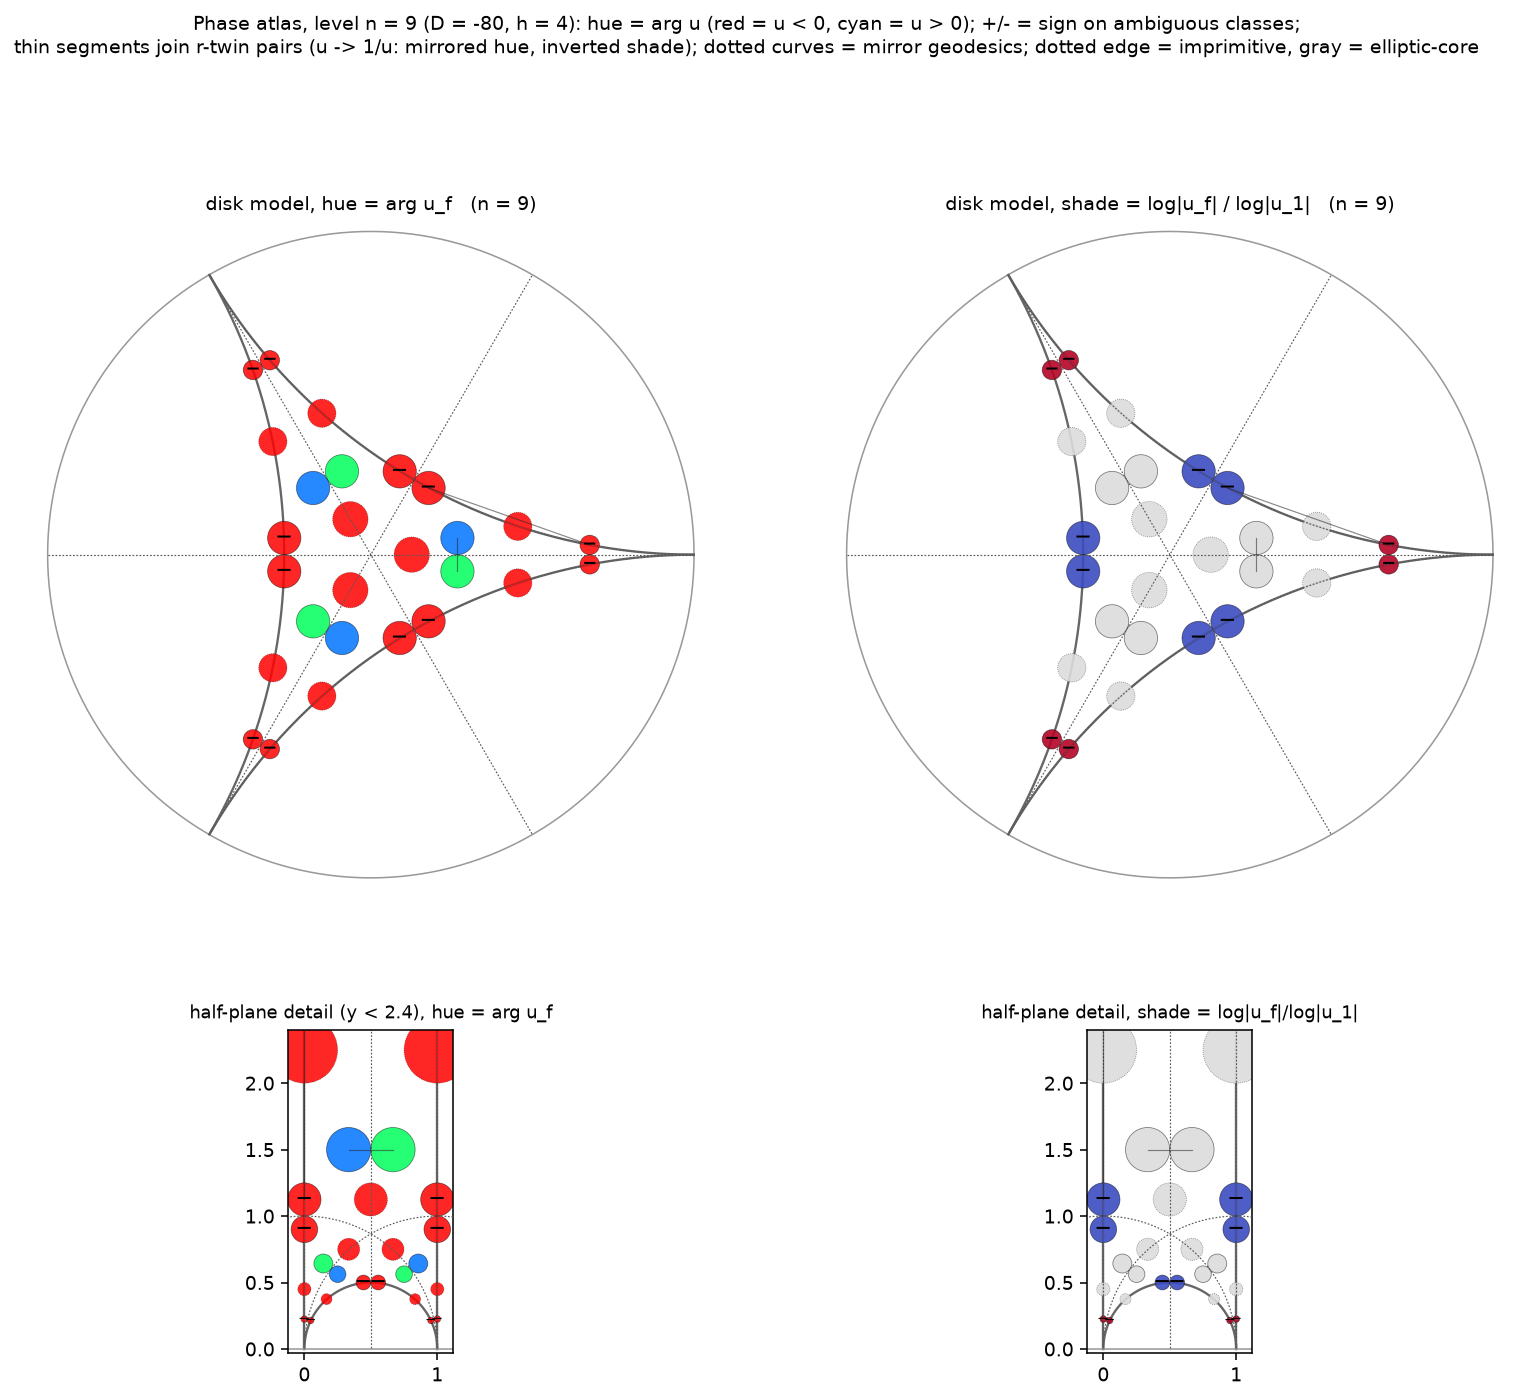
\includegraphics[width=0.9\textwidth]{phase-atlas-n9.png}
\caption{The phase portrait of level $n = 9$ (discriminant $-80$,
class group $\Z/4$): the circles of the ideal triangle colored by
$\arg u_f$ (hue) and $\log|u_f|/\log|u_1|$ (shade), with mirror
geodesics overlaid.  Level $9$ is the first level with non-real
phases.  Mirror-image circles carry conjugate hues (law 1);
$\idealr_n$-twin pairs carry mirrored hues and inverted shades (law
2).  Produced by \texttt{make\_phase\_atlas.py}.}
\label{fig:atlas9}
\end{figure}

\subsection{The phase is not cycle-integral data: the
Duke--Imamo\u{g}lu--T\'oth comparison}\label{subsec:dit}

The level-$n$ data lives on the real quadratic side through the Cartan
geodesic: trace $-2n$, length $2\log\varepsilon_n$, discriminant
$d = 4(n^2 - 1) = -4D$.  The alignment is exact: the minimal solution
of $t^2 - du^2 = 4$ is $(t, u) = (2n, 1)$, so the fundamental
automorph of every form of discriminant $d$ is $\varepsilon_n$ itself
--- the unit that normalizes the phase.  The invariants classically
attached to such $d$ are the cycle integrals of Duke, Imamo\u{g}lu and
T\'oth \cite{DIT2011}: for each form class $A$ of discriminant $d$,
$C_A(f) = \int_{\Gamma_Q\backslash S_Q} f(z)\,\tfrac{\sqrt
d\,dz}{Q(z, 1)}$ for $f = j - 744$, together with the Kronecker-limit
integrals $E_A$ (the same integral for $f = \log(\im(z)^6
|\Delta(z)|)$) and the Rademacher symbols $\Psi(\gamma_A)$ of the
automorphs; and the coupled pair $(D, d) = (1 - n^2,\, 4(n^2-1))$ of
discriminants of opposite sign is precisely the index shape of the
two-sign Fourier coefficients in the Katok--Sarnak framework
\cite{KatokSarnak1993}.  It is natural to ask whether the phase is a
linear shadow of these invariants.  It is not:

\begin{proposition}[computational: certified non-relation]
\label{prop:dit}
For every odd $3 \le n \le 17$, compute all cycle integrals
$C_A(j - 744)$ and $E_A$ over the $\SL_2(\Z)$-classes of discriminant
$4(n^2 - 1)$ (from the definitions, validated by $C_A(1) =
2\log\varepsilon_A$, independent parametrizations, and
$\SL_2(\Z)$-invariance to $10^{-140}$), and the phases $u_f$ at $170$
digits.  Integer-relation searches (PSLQ) at $150$-digit working
precision, accepting a candidate only when
$(\text{terms})\times(\text{coefficient digits})$ is far below the
working precision, find \textbf{no relation} in any of the following
tests: $\log|u_f|$ against $[1, \log\varepsilon,
\mathrm{Tr}_d(j{-}744), \sum_A E_A, \pi^2]$ (coefficient bound
$10^8$); $\log|u_f|$ against $[1, \log\varepsilon]$ (bound $10^{10}$;
so $u_f$ is not $\pm\,\text{rational}\times\varepsilon^k$ in
disguise); $\log|u_f|$ against the per-class $\re C_A(j{-}744)$ and
$E_A$ (bound $10^6$); the argument $\arg u_f$ against
$[\pi, \log\varepsilon]$, and against the per-class
$\im C_A(j{-}744)$ and $\pi$; and the pair-sums
$S_x$ against the aggregate basis --- across the full battery, $52$
certified non-relations, zero unsafe candidates, and the only
target-involving hit is the proved anchor $u = -1$ at $n = 3$.
Moreover the Rademacher symbols on the trace-$2n$ classes are
antisymmetric under class inversion (so $\sum_A \Psi_A = 0$
identically), while $\sgn(u_f)$ lives on the imaginary-quadratic
$2$-torsion and is not even a character: no per-class matching is
possible.  \emph{(Script \texttt{dit\_comparison.py}; re-run for this
paper.)}
\end{proposition}

This is the expected outcome, and the structural reason deserves
record: $u_f$ is \emph{algebraic} (Theorem \ref{thm:firstpower}),
while cycle integrals of $j$ are expected to be transcendental and are
not known to be logarithms of algebraic numbers; a nontrivial linear
identity would have been a transcendence miracle.  The value of the
certified mismatch is the license it gives: the phase is genuinely new
real-quadratic-adjacent data at $d = 4(n^2 - 1)$, not repackaged
cycle-integral material.  What the two theories \emph{do} share ---
exactly $\varepsilon_n$, the coupled pair $(D, -4D)$, and the
$E_6$-geometry at the elliptic point (Theorem \ref{thm:signlaw}) ---
marks the structured place to look next: mixed objects indexed by a
pair of discriminants of opposite sign, in the sense of
\cite{KatokSarnak1993}, rather than the one-discriminant invariants
tested here.

%%% ============================================================
\section{The Euclidean phase}\label{sec:euclidean}

The phase of Section \ref{sec:phase} was a two-sided
$\SL_2(\Z)$-invariant.  Replacing the left factor by the
\emph{Euclidean symmetries of the plane inside the Bianchi group} ---
the translations $N = \{T_{\alpha} = \begin{pmatrix} 1 & \alpha \\ 0 &
1 \end{pmatrix} : \alpha \in \Zi\}$ --- produces a parallel theory
with an even cleaner mechanism, and, remarkably, with complete
answers: its level polynomials are monic and irreducible for every
level.  We study functions of $X$ invariant under $X \mapsto
T_{\alpha}X\gamma'$, $\alpha \in \Zi$, $\gamma' \in \SL_2(\Z)$.

\subsection{The moduli problem and the sixth invariant}
\label{subsec:eucmoduli}

Let $X = \begin{pmatrix} a & b \\ c & d\end{pmatrix} \in \SL_2(\C)$
with $c \ne 0$ and $X(\HH)$ a \emph{bounded disk} $D$; boundedness is
equivalent to $\kappa := 2\im(\bar cd) > 0$, equivalently
$w := d/c = -X^{-1}(\infty) \in \HH$, and $\kappa$ is then the
curvature of $\partial D$.  For $X \in \SL_2(\Zi)$ this is the
positive-curvature normalization of a Schmidt disk: $\kappa = 2n$,
center $\zeta/2n$, $\zeta \equiv i \pmod 2$.  Two invariants are
visible at once: the circle modulo $\Zi$-translation (the Cartan datum;
three real parameters) and
\[
  \beta(X) := j(w) = j\bigl(-X^{-1}(\infty)\bigr)
\]
(two more; left translations do not touch the bottom row, and right
multiplication moves $w$ by an element of $\SL_2(\Z)$).  Five real
parameters in all.  What they miss: the double coset of a generic $X$
is described by the oriented lattice $\Lambda = \Z c + \Z d \subset
\C$ together with the center of the disk mod $\Zi$; of the lattice,
the five invariants see the covolume ($= \kappa/2$) and the homothety
class ($= j(w)$) but \emph{not the phase of the homothety}.  That
missing dimension is the sixth invariant:

\begin{definition}\label{def:euctheta}
$\displaystyle
\Theta(X) := \frac{j'(w)}{c^2}
= -\operatorname*{Res}_{z = X^{-1}(\infty)}X(z)\cdot
j'\bigl(-X^{-1}(\infty)\bigr)$.
\end{definition}

\begin{proposition}\label{prop:eucinv}
$\Theta(T_{\alpha}X\gamma') = \Theta(X)$ for every $\alpha \in \C$
(not just $\Zi$) and every $\gamma' \in \SL_2(\Z)$.  In lattice terms,
$\Theta(X) = \hat h_2(\Lambda_X)$, where $\hat h_2(\Z c + \Z d) :=
j'(d/c)/c^2$ is the weight-$2$ homogeneous extension of $j'$ to
oriented lattices: \emph{the sixth invariant is the weight-$2$ value
at the actual lattice}, not just at its homothety class.  Fixing the
five invariants, the identity component of the fiber is $X\{h_t\}$
with $h_t$ the rotation group fixing the pole; along it $|\Theta|$ is
constant and $\arg\Theta$ moves linearly at rate $2$ (the weight).
Finally, the full stabilizer of $\infty$ in $\PSL_2(\Zi)$ is generated
by $N$ and $z \mapsto -z$, which sends $D \mapsto -D$ and $\Theta
\mapsto -\Theta$: the two disks $\pm D$ carry opposite phases.
\end{proposition}

\begin{proof}
Left translations do not touch $(c, d)$.  On the right, $(c, d)
\mapsto (cp + dr, cq + ds)$, so $w$ moves by an $\SL_2(\Z)$-M\"obius
map and $c \mapsto c(p + rw)$; the weight-$2$ law for $j'$ cancels the
factor $(p + rw)^2$.  Basis-independence of $\hat h_2$ \emph{is} this
right-invariance.  For the fiber: a real $h$ preserves the circle
exactly iff it fixes the pole; the generator of that elliptic group
has row eigenvector $(1, w)$ with unit-modulus eigenvalue $e^{-it}$,
so the bottom row $(c, d) = c(1, w)$ transforms by $c \mapsto
ce^{-it}$, fixing $w$ and $|c|$ and rotating $\Theta = j'(w)/c^2$ at
rate $2$.  The Borel sign is the computation
$\operatorname{diag}(i, -i)$: $(c, d) \mapsto (-ic, -id)$, $c^2
\mapsto -c^2$.
\end{proof}

This is the exact structural analogue of the hyperbolic phase: there,
two kernels (one per $\SL_2(\Z)$-factor) glued by a derivative; here,
one kernel glued by a residue --- the left factor is a translation
group, whose derivative is $1$ and which needs no kernel.

\subsection{Structure of a level: conductor $=$ curvature}
\label{subsec:eucstructure}

Let $K = \Q(i)$, $\mathcal{O}_n = \Z + n\Zi$ the order of conductor
$n$ and discriminant $-4n^2$, $h(-4n^2)$ its class number.

\begin{lemma}[disk $\leftrightarrow$ lattice]\label{lem:disklattice}
$D \mapsto \Lambda_D = \Z c + \Z d$ is a bijection from Schmidt disks
of curvature $2n$ modulo $\Zi$-translation onto the primitive index-$n$
sublattices $\Lambda \subseteq \Zi$ (primitive: $\Lambda\Zi = \Zi$).
\end{lemma}

\begin{proof}
$D$ determines $X$ up to $X \mapsto T_{\lambda}Xh$, $h \in
\pm\SL_2(\Z)$, so the oriented lattice is well defined; it has index
$|\im(\bar cd)| = n$ and is primitive because $ad - bc = 1 \in (c,
d)$.  Conversely an oriented basis of a primitive $\Lambda$ has
$\gcd_{\Zi}(c, d) = 1$, hence completes to $X \in \SL_2(\Zi)$, and the
completions form exactly one translation class (replacing the top row
by $(a + tc, b + td)$ translates the disk by $t$).
\end{proof}

\begin{lemma}[conductor $=$ curvature]\label{lem:conductor}
Every primitive index-$n$ sublattice $\Lambda \subseteq \Zi$ is a
proper $\mathcal{O}_n$-lattice: its multiplier ring is exactly
$\Z + n\Zi$.
\end{lemma}

\begin{proof}
Primitivity forces $\Zi/\Lambda$ cyclic, so $\Lambda = \ker\phi$ for a
surjection $\phi(x + yi) = sx + ty$ onto $\Z/n$, $\gcd(s, t, n) = 1$.
Eliminating the scalar by which $x + yi$ acts on the cyclic quotient
gives $x + yi \in \mathcal{O}(\Lambda) \iff n \mid y(s^2 + t^2)$, so
the conductor is $n/\gcd(n, s^2 + t^2)$.  For $p \mid n$: $p \mid s^2
+ t^2$ iff the line $\ker(\phi \bmod p)$ is an ideal line of $\Zi/p$,
and primitivity excludes exactly the ideal lines; hence $\gcd(n, s^2 +
t^2) = 1$.
\end{proof}

(The count of surviving lines --- $p + 1$ minus $0/1/2$ ideal lines at
inert/ramified/split $p$ --- re-derives $N_e(n)$ of Proposition
\ref{prop:Ne} from scratch.)

\begin{lemma}[every class, exactly twice]\label{lem:everyclasstwice}
For $n \ge 2$, the class map $\Lambda \mapsto [\Lambda] \in
\Cl(\mathcal{O}_n)$ from primitive index-$n$ sublattices is surjective
with all fibers $\{\Lambda, i\Lambda\}$ of size two; the corresponding
disk pairs are $\{D, -D\}$.
\end{lemma}

\begin{proof}
Given a class, pick an integral representative $\ideala$ prime to
$n$ and a generator $\alpha$ of $\ideala\Zi$ ($\Zi$ is a PID); then
$\Lambda = \alpha^{-1}\ideala \subseteq \Zi$ is primitive, proper for
$\mathcal{O}_n$, of index $n$ (extension of ideals prime to the
conductor preserves norms), and the construction is independent of
choices up to $\mu_4$, with $-\Lambda = \Lambda$ and $i\Lambda \ne
\Lambda$ (else $i \in \mathcal{O}(\Lambda) = \mathcal{O}_n$).
Conversely every primitive $\Lambda$ arises from its own class.
Finally $i\Lambda$ is the lattice of $-D$, and homothety by $i$ does
not change the class.
\end{proof}

\begin{theorem}[Euclidean structure]\label{thm:euclidstructure}
For $n \ge 2$, the assignment $D \mapsto [\Lambda_D]$ induces a
bijection
\[
  \bigl\{\text{curvature-}2n \text{ Schmidt disks in } [0,1) +
  [0,1)i\bigr\}\big/(z \mapsto -z)
  \;\xrightarrow{\ \sim\ }\; \Cl(\Z + n\Zi),
\]
and in particular $N_e(n) = 2h(-4n^2)$ for $n \ge 2$ (and $N_e(1) =
h(-4) = 1$).  Under the bijection, complex conjugation of disks is
inversion in the class group, and the disks tangent to $\Rhat$ (the
Ford row, $\zeta = \pm i$) are the principal class, with $w \sim ni$.
\end{theorem}

For $K = \Q(i)$ this is equivalent to Stange's theorem
\cite{StangeIMRN} that circles of curvature $f\sqrt{-\Delta}$, up to
translation and rotation by $180^{\circ}$, are in bijection with
$\ker(\Pic(\mathcal{O}_f) \to \Pic(\mathcal{O}_K))$ --- for class
number one, all of $\Pic(\mathcal{O}_f)$.  The proof above (Lemmas
\ref{lem:disklattice}--\ref{lem:everyclasstwice}) gives the explicit
dictionary the phase theory needs.  The count identity reconciles the
multiplicative formula of Proposition \ref{prop:Ne} with the class
number formula for orders: \emph{the Euclidean census of the Gaussian
Schmidt arrangement is a class number census of the non-maximal orders
of $\Q(i)$}.

\begin{theorem}[singular moduli of the Euclidean family]
\label{thm:eucj}
For $n \ge 2$,
\[
  \prod_{\substack{D \text{ Schmidt disk of curvature } 2n\\
  \text{center} \in [0,1) + [0,1)i}}
  \bigl(x - j(-X_D^{-1}(\infty))\bigr)
  \;=\; H_{-4n^2}(x)^2 \;\in\; \Z[x],
\]
the square of the ring class polynomial of $\Z + n\Zi$; for $n = 1$ it
is $H_{-4}(x) = x - 1728$.
\end{theorem}

\begin{proof}
$w = d/c$ is a CM point of $\Q(i)$ whose order is exactly
$\mathcal{O}_n$ by Lemma \ref{lem:conductor}, and $j(w) =
j([\Lambda_D])$; by Theorem \ref{thm:euclidstructure} the disks of the
level sweep each class exactly twice.
\end{proof}

The anchors are classical: the Ford disks see $j(i) = 1728$; the
curvature-$4$ disks see $j(2i) = 66^3$.  At hyperbolic level $n$ the
$\beta$-values were singular moduli of discriminant $1 - n^2$ (fixed
maximal-order type, field varying with the level); at Euclidean
curvature $2n$ they are singular moduli of conductor $n$ over the
fixed field $\Q(i)$: \emph{the arrangement sees, along its two natural
gradings, the two orthogonal aspects of complex multiplication ---
discriminant and conductor.}

\begin{proposition}[traces: the even-square slice; computational]
\label{prop:euctraces}
Set $\mathrm{Tr}^E_n := \sum_{\idealc}(j(\idealc) - 744)$ over
$\Cl(\mathcal{O}_n)$ for $n \ge 2$, and
$\mathrm{Tr}^E_1 := 492$, one has $\sum_{g \mid n}\mathrm{Tr}^E_{n/g}
= t(4n^2)$, Zagier's trace \cite{Zagier2002}; verified for all
$n \le 13$ by \texttt{euclidean\_\allowbreak moduli\_\allowbreak invariants.py}.  The Euclidean
census reads the weight-$3/2$ coefficients along the even squares
$d = 4n^2$, the complementary diagonal to the hyperbolic slice.
\end{proposition}

\subsection{The lemniscatic phase}\label{subsec:lemniscatic}

On integral $X$ the five invariants produce ring class integers; the
sixth is transcendental --- but by exactly one period.  Define
\[
  \Omega := \frac{\Gamma(\tfrac14)^4}{8\pi^2} = \frac{\varpi^2}{\pi}
  = \bigl((2\pi)^6\eta(i)^{24}\bigr)^{1/6} = 2.18843961\ldots,
  \qquad
  u(D) := \frac{\Theta(X_D)}{\Omega},
\]
where $\varpi = 2\int_0^1 dt/\sqrt{1 - t^4}$ is the lemniscate
constant --- the period of the CM curve $\C/\Zi$, whose homothety
class is the unique class at $n = 1$.  From $j'^{\,6} =
-(2\pi)^6j^4(j - 1728)^3\Delta$,
\begin{equation}\label{eq:u6}
  u(D)^6 \;=\; -\,\beta^4(\beta - 1728)^3\,
  \frac{\Delta(\Lambda_D)}{\Delta(\Zi)}, \qquad \beta = j(w_D),
\end{equation}
where $\Delta(\Lambda)$ is the weight-$12$ lattice discriminant.  The
$\Delta$-quotient of commensurable CM lattices is algebraic and
$n^{12}\Delta(\Lambda)/\Delta(\Zi)$ is an algebraic integer
\cite[Ch.~12]{Lang1987}, so \emph{$u(D)$ is algebraic and $n^2u(D)$ an
algebraic integer}.

\begin{example}[the anchor $n = 2$: an exact integer phase]
For the curvature-$4$ disks, $\beta = 66^3$, $\beta - 1728 =
2^33^67^2$, and $\Delta(\Lambda)/\Delta(\Zi) = \eta(2i)^{24}/
\eta(i)^{24} = 2^{-9}$, giving $u^2 = -2^43^{10}7^211^4$ exactly:
\[
  u = \pm\,2^23^5\cdot 7\cdot 11^2\,i = \pm\,823284\,i .
\]
This is the Euclidean analogue of the hyperbolic anchor $u = -1$ at
$n = 3$ --- with the characteristic difference that the Euclidean
phase is an $S$-integer rather than a unit.
\end{example}

\begin{proposition}[laws and the reality criterion]\label{prop:euclaws}
For every Schmidt disk $D$ of curvature $2n \ge 4$:
\begin{enumerate}
\item $u(-D) = -u(D)$: the two disks of a class carry opposite phases,
so $u^2$ is well defined on $\Cl(\mathcal{O}_n)$; write
$v_{\idealc}^2$.
\item $u(\bar D) = \overline{u(D)}$ and $[\Lambda_{\bar D}] =
[\Lambda_D]^{-1}$: conjugation of disks is inversion in the class
group.
\item On an ambiguous class, $u \in \R \cup i\R$; precisely, with
$\zeta = x + yi$ the curvature-center of either disk of the class,
\[
  u \in \R \iff n \mid y, \qquad u \in i\R \iff n \mid x,
\]
and for $n \ge 2$ exactly one of the two holds on each ambiguous
class.  Since $y$ is odd, even levels have no real classes; at every
odd $n \ge 3$ the class of $\zeta = (n + 1) + ni$ is real.
\end{enumerate}
\end{proposition}

\begin{proof}
(1) is the Borel sign of Proposition \ref{prop:eucinv}.  (2) $\bar D =
Y(\HH)$ for $Y = \bar X\operatorname{diag}(i, -i)$, with invariant
point $w_Y = -\bar w$; the real-kernel identity $j'(-\bar\tau) =
-\overline{j'(\tau)}$ combines the factors to $\Theta(Y) =
\overline{\Theta(X)}$, and $\bar\Lambda$ represents the conjugate,
i.e.\ inverse, class.  (3) Ambiguity means $\bar\zeta \equiv \pm\zeta
\pmod{2n}$, i.e.\ $n \mid y$ resp.\ $n \mid x$; then (2) and (1) give
$\bar u = u$ resp.\ $\bar u = -u$.  Both together would force $n^2
\mid x^2 + y^2 \equiv 1 \pmod{4n}$, impossible for $n \ge 2$.
Solvability at $y = n$: $x = n + 1$ works for every odd $n$.
\end{proof}

\subsection{One level, one monic integer polynomial}
\label{subsec:eucpoly}

\begin{theorem}[sixth powers, unconditionally]\label{thm:P6}
Fix $n \ge 2$ and let $v_{\idealc}$ ($\idealc \in \Cl(\mathcal{O}_n)$)
be the phases, each taken at either disk of its class.  Then
\[
  P^{(6)}_n(y) := \prod_{\idealc \in \Cl(\mathcal{O}_n)}
  \bigl(y - (n^2v_{\idealc})^6\bigr) \;\in\; \Z[y],
\]
monic of degree $h(-4n^2)$, and the product over all $2h$ disks of the
level is $P^{(6)}_n(y)^2$.
\end{theorem}

\begin{proof}
(i) \emph{Rationality.}  For $\tau \in \HH$ and a cyclic index-$n$
sublattice $\Lambda_{a,b,d} = \Z(a\tau + b) + \Z d \subset \Z\tau +
\Z$ ($ad = n$, $\gcd(a, b, d) = 1$), the quantity
\[
  F_{a,b,d}(\tau) := \frac{n^{12}\,\hat h_2(\Lambda_{a,b,d})^6}
  {(2\pi)^6\Delta(\tau)}
  = -\,\frac{n^{12}}{d^{12}}\,j_w^4(j_w - 1728)^3\,
  \frac{\Delta(w)}{\Delta(\tau)}, \qquad w = \tfrac{a\tau + b}{d},
\]
is one member of a Hecke orbit: $\SL_2(\Z)$ permutes the
$F_{a,b,d}$, so every elementary symmetric function of them (jointly
with the $j_w$) is a meromorphic modular function, holomorphic off the
cusp, with rational $q$-expansion (the root-of-unity coefficients
cancel in the symmetrization over $b$, exactly as for the classical
modular polynomials) --- hence a polynomial in $j(\tau)$ with rational
coefficients.  Evaluating at $\tau = i$ ($j = 1728$) makes all
symmetric functions of the cyclic family rational, jointly with the
$\beta$'s.  (ii) \emph{The primitive cut.}  By Lemma
\ref{lem:conductor} the primitive sublattices are exactly the cyclic
ones whose $\beta$ has discriminant $-4n^2$; the discriminant of
$\beta$'s order is a Galois invariant, so $\Gal(\bar\Q/\Q)$, which
permutes the joint pairs $(\beta_{\Lambda}, F_{\Lambda})$, preserves
the primitive sub-multiset, whose symmetric functions are therefore
rational.  Each class appears twice with the same sixth power.
(iii) \emph{Integrality.}  $\beta$ and $\beta - 1728$ are algebraic
integers and $n^{12}\Delta(\Lambda)/\Delta(\Zi)$ is an algebraic
integer; a monic rational polynomial with algebraic-integer roots lies
in $\Z[y]$.
\end{proof}

Contrast with Theorem \ref{thm:levelpoly}: same shape --- one level,
one integer polynomial --- but the Euclidean polynomial is
\emph{monic}: the hyperbolic denominators came from kernel values at
two CM points in a ratio; here there is one kernel value, its
elliptic-point factors $\beta^4(\beta - 1728)^3$ sit in the
numerator, and all denominators live over $n$, cleared by $n^2$.

Experimentally the descent to \emph{squares} holds at every computed
level with a smaller normalizer: let $\lambda_n$ be the least positive
integer with $P^{(2)}_n(y) := \prod_{\idealc}(y -
(\lambda_nv_{\idealc})^2) \in \Z[y]$.  Certified values
(\texttt{euclidean\_moduli\_invariants.py}, $140$--$840$ digits,
absolute-error criterion) include
\begin{gather*}
  P^{(2)}_2(y) = y + 2^43^{10}7^211^4 \quad (\lambda_2 = 1),\\
  P^{(2)}_3(y) = y^2 + 194359980365709312\,y - \cdots \quad
  (\lambda_3 = 1),
\end{gather*}
with
\[
\begin{array}{c|cccccccccccc}
n & 2 & 3 & 4 & 5 & 6 & 7 & 8 & 9 & 10 & 11 & 12 & 13\\
\hline
h(-4n^2) & 1 & 2 & 2 & 2 & 4 & 4 & 4 & 6 & 4 & 6 & 8 & 6\\
\lambda_n & 1 & 1 & 4 & 25 & 1 & 49 & 2^5 & 3^3 & 25 & 11^2 & 4 &
13^2
\end{array}
\]
The rationality and irreducibility at square level are in fact
theorems for every $n$, by the following three steps.

\begin{lemma}[the root-free closed form]\label{lem:g2form}
$\displaystyle
u_{\idealc}^2 \;=\; -\,12\;\beta_{\idealc}\,(\beta_{\idealc} - 1728)\,
\frac{g_2(\Lambda_{\idealc})}{g_2(\Zi)}$ --- a ring class integer
times a weight-balanced ratio of Weierstrass $g_2$-values at the pair
$\Lambda_{\idealc} \subset \Zi$, with no root of any modular form
extracted anywhere.
\end{lemma}

\begin{proof}
$j'(\tau)^2 = -(2\pi)^2 j(\tau)(j(\tau) - 1728)E_4(\tau)$ from $j' =
-2\pi i\,E_4^2E_6/\Delta$ and $E_4^3 = j\Delta$, $E_6^2 = (j -
1728)\Delta$; and $\Omega^2 = (2\pi)^2\eta(i)^8 = (2\pi)^2E_4(i)/12$
since $\gamma_2(i) = 12$.  Homogenize.
\end{proof}

\begin{lemma}[transport of balanced pair-values]\label{lem:lemmaT}
Let $F(\Lambda; L)$ be a rational expression in $g_2, g_3$ of two
lattices, isobaric of total weight $0$ under joint scaling.  For
$\sigma \in \operatorname{Aut}(\C/K)$ with id\`ele $s$ and any pair of
$K$-lattices $\Lambda \subseteq L$ of index $n$:
\[
  \sigma\bigl(F(\Lambda; L)\bigr) = F\bigl(s^{-1}\Lambda;\,
  s^{-1}L\bigr),
\]
the adelic action preserving index, multiplier orders, and (up to the
class of $s$) proper-ideal classes.
\end{lemma}

\begin{proof}
Let $E = E_{\Lambda}$, $E' = E_L$ be the Weierstrass curves and
$\phi: E \to E'$ the isogeny that is analytically $z \mapsto z$, so
$\phi^*\omega' = \omega$ for the Weierstrass differentials.  By the
main theorem of complex multiplication in Shimura's formulation for
arbitrary lattices \cite[Thm.~5.4]{Shimura1971}, $E^{\sigma}$ is
analytically $\C/s^{-1}\Lambda$ via a parametrization compatible with
$\sigma$ on torsion, and likewise $E'^{\sigma}$; compatibility on the
dense torsion forces $\phi^{\sigma}$ to be analytically $z \mapsto z$.
Writing $\Lambda_1, L_1$ for the exact period lattices of the
transformed Weierstrass equations, $\Lambda_1 =
\theta_E\,s^{-1}\Lambda$ and $L_1 = \theta_{E'}s^{-1}L$, and
$\phi^{\sigma}$ is multiplication by $\theta_{E'}\theta_E^{-1}$; but
$\sigma$ commutes with algebraic pullback of the algebraically defined
$\omega$, so $(\phi^{\sigma})^*\omega_{L_1} = \omega_{\Lambda_1}$,
i.e.\ $\theta_{E'} = \theta_E$: the transformed pair is \emph{jointly}
homothetic to $(s^{-1}\Lambda, s^{-1}L)$.  Joint scaling invariance of
$F$ finishes.
\end{proof}

\begin{proposition}[translation law at square level; no cocycle]
\label{prop:euctranslation}
For $\sigma \in \Gal(\bar\Q/K)$ with Artin class $\idealc(\sigma) \in
\Cl(\mathcal{O}_n) \cong \Gal(H_n/K)$:
\[
  \sigma\bigl(u^2_{\idealc}\bigr) = u^2_{\idealc(\sigma)^{-1}
  \idealc}\,;
\]
in particular $u^2_{\idealc} \in H_n$, and with the mirror law
(Proposition \ref{prop:euclaws}) the full group $\Gal(\bar\Q/\Q)$
permutes $\{u^2_{\idealc}\}$ through the generalized dihedral action.
\end{proposition}

\begin{proof}
Lemma \ref{lem:g2form} exhibits $u^2_{\idealc}$ as
$\beta(\beta - 1728)$ times $F(\Lambda_{\idealc}; \Zi)$ with $F =
-12\,g_2(\Lambda)/g_2(L)$, isobaric of joint weight $0$.  Apply
$\sigma$: the $\beta$-factor translates by ring class reciprocity
\cite[Thm.~11.36]{Cox2013}, and Lemma \ref{lem:lemmaT} gives $\sigma F
= F(s^{-1}\Lambda_{\idealc}; s^{-1}\Zi)$.  Rescale jointly by a
generator $\nu$ of the principal ideal $(s^{-1}\Zi)^{-1}$: $\Lambda' =
\nu s^{-1}\Lambda_{\idealc}$ is primitive of index $n$ with
$[\Lambda'] = \idealc(\sigma)^{-1}\idealc$, and $\sigma F =
F(\Lambda'; \Zi)$, the $u^2$-datum of that class.  The representative
$\Lambda'$ is determined up to $\mu_4$, and $F$ has weight $4$ in
$\Lambda$ alone, so $i^{-4} = 1$ kills the ambiguity: at square level
there is no cocycle at all.
\end{proof}

\begin{lemma}[archimedean dominance of the principal class]
\label{lem:dominance}
For every $n \ge 2$ and every class $\idealc \ne 1$:
$|u_{\idealc}| < |u_1|$; explicitly $|u_{\idealc}|/|u_1| \le
10\,e^{-\pi n}$.
\end{lemma}

\begin{proof}
By Proposition \ref{prop:eucinv}, $|u_{\idealc}| =
|j'(\tau_{\idealc})|/(A_{\idealc}\Omega)$ at the reduced CM point
$\tau_{\idealc} = \tfrac{-B + 2ni}{2A}$, with $A_1 = 1$ and
$A_{\idealc} \ge 2$ for $\idealc \ne 1$ (a reduced form of even
discriminant with $A = 1$ has $B = 0$, hence is principal).  On the
fundamental domain $|q| \le e^{-\pi\sqrt3} < \tfrac1{230}$, and the
crude bounds $\sigma_3(k) \le k^4$, $\sigma_5(k) \le k^6$ give $|E_4|
\le 2.12$, $|E_6| \le 3.9$, $|\Delta_q| \ge 0.90\,|q|$, so $|j'| \le
2\pi\cdot 19.5\,e^{2\pi y}$; at $\tau = ni$ ($q = e^{-2\pi n} > 0$,
$n \ge 2$): $E_4 \ge 1$, $E_6 \ge 0.998$, $\Delta_q \le q$, so
$|j'(ni)| \ge 2\pi\cdot 0.998\,e^{2\pi n}$.  Hence
$|u_{\idealc}|/|u_1| \le \tfrac{19.5}{0.998}\cdot\tfrac1A
e^{2\pi n(\frac1A - 1)} \le 10e^{-\pi n} < \tfrac1{50}$.
\end{proof}

\begin{theorem}[irreducibility at every level]\label{thm:euclideanirred}
For every $n \ge 2$:
\begin{enumerate}
\item $\Gal(\bar\Q/\Q)$ permutes $\{u^2_{\idealc}\}$ generalized
dihedrally; hence $\prod_{\idealc}(y - (n^2v_{\idealc})^2)$ is a monic
integer polynomial for all $n$.
\item $P^{(2)}_n$ is irreducible over $\Q$ (in any rational
normalization of the roots): the square-phases of a level form a
single Galois orbit, $[\Q(v^2_{\idealc}) : \Q] = h(-4n^2)$ with
$v^2_{\idealc} \in H_n$, and the Galois image is contained in (at the
computed levels: equal to) the generalized dihedral group of
$\Cl(\mathcal{O}_n)$.
\item The same holds for $P^{(6)}_n$.
\end{enumerate}
\end{theorem}

\begin{proof}
(1) Stability under $\Gal(\bar\Q/K)$ is Proposition
\ref{prop:euctranslation}; complex conjugation is the mirror law; any
other $\sigma$ is a composite.  Symmetric functions are then rational,
and the roots $(n^2v_{\idealc})^2$ are algebraic integers.  (2) By
Artin surjectivity the translations act transitively, so all
$u^2_{\idealc}$ are conjugate and $P^{(2)}_n = m^{|T|}$ with $m$
irreducible and $T = \{\mathfrak{t} : u^2_{\mathfrak{t}} = u^2_1\}$ a
subgroup (the coincidence relation is translation-invariant).  Any
$\mathfrak{t} \in T$ has $|u_{\mathfrak{t}}| = |u_1|$, so Lemma
\ref{lem:dominance} forces $T = 1$.  (3) Cube the translation law; the
same dominance argument applies.
\end{proof}

The mechanism deserves note.  The two hypotheses that remain open on
the hyperbolic side (Open problem \ref{op:distinct} and the historical
first-power descent) both evaporate here: the descent because the
square-phase has the root-free $g_2$-form, and $T = 1$ because the
coincidence set is a subgroup, so it only had to be tested against the
archimedeanly dominant principal class --- and the principal class is
the row of disks tangent to $\Rhat$, whose CM point $ni$ escapes to
the cusp while every other class stays at height $\le n/2$.  \emph{The
tangency geometry of the arrangement pins the factorization type.}

\begin{remark}[first powers; computational, open in general]
\label{rem:eucfirstpower}
The disk-level multiset $\{\lambda_nu(D)\}$ is $\{\pm\lambda_n
v_{\idealc}\}$, the root set of $P^{(2)}_n(x^2) \in \Z[x]$ of degree
$2h = N_e(n)$.  At every computed level $2 \le n \le 16$ this
polynomial is \emph{irreducible} (exact factorization;
\texttt{mass\_law\_and\_irreducibility.py}): the $N_e(n)$ normalized
phases of a level --- one per disk in the unit square --- form a
single Galois orbit and $[\Q(\lambda_nv_{\idealc}) : \Q] = N_e(n)$;
passing from $v^2$ to $v$ always doubles the degree.  Whether this
first-power irreducibility holds for all $n$ is open: the natural
attack is a weight-$2$ refinement of Lemma \ref{lem:lemmaT}, where the
$\mu_4$-ambiguity survives as a genuine $\pm$-cocycle tied to the
orientation data --- the exact Euclidean shadow of the hyperbolic
first-power problem, one power lower than what Theorem
\ref{thm:euclideanirred} settles.
\end{remark}

\subsection{The $\Delta$-mass law}\label{subsec:massa}

The proof of Theorem \ref{thm:euclideanirred} controls the Galois
theory of a level; the following exact product law controls its
absolute values.  Define the \emph{$\Delta$-mass}
\[
  M(n) \;:=\; \prod_{\idealc \in \Cl(\mathcal{O}_n)}
  n^{12}\,\frac{\Delta(\Lambda_{\idealc})}{\Delta(\Zi)} .
\]

\begin{theorem}[$\Delta$-mass law]\label{thm:massa}
For every $n \ge 2$,
\[
  M(n) \;=\; \varepsilon(n)\prod_{\substack{p^k \parallel n\\ p
  \text{ not split}}} p^{\;\frac{6}{e_p}\cdot\frac{p^k - 1}{p - 1}\,
  N_e(n/p^k)},
  \qquad
  \varepsilon(n) = \begin{cases} -1 & n = 2^k,\ k \ge 2,\\ +1 &
  \text{otherwise,}\end{cases}
\]
with $e_2 = 2$ (ramified) and $e_p = 1$ (inert); split primes
contribute nothing at all --- e.g.\ $M(5) = M(13) = M(25) = 1$
exactly.
\end{theorem}

\begin{proof}
Four steps; each is separately machine-verified by the script
\texttt{mass\_\allowbreak law\_\allowbreak and\_\allowbreak irreducibility.py}.

\emph{(M1) The full mass is a constant.}  For $\tau \in \HH$ let
$A(n)(\tau) := \prod_{\Lambda}\Delta(\Lambda)/\Delta(L_{\tau})$, the
product over \emph{all} $\sigma(n)$ index-$n$
sublattices $\Lambda$ of $L_{\tau} = \Z\tau + \Z$.  The family is
lattice-intrinsic and $\Delta$-ratios are homothety-invariant, so
$A(n)$ is $\SL_2(\Z)$-invariant; in the Hermite parametrization each
factor is holomorphic and nonvanishing on $\HH$ and meromorphic at the
cusp, so $A(n)$ is a rational function of $j$ with no zeros or poles
in $\C$ --- a constant, equal to its $q \to 0$ limit.  The factor
$(a, b, d)$ contributes leading term $d^{-12}\zeta_d^bq^{a/d - 1}$;
the $q$-exponents cancel ($\sum_{ad = n}(a - d) = 0$) and
$\zeta_d^{0 + 1 + \cdots + (d - 1)} = (-1)^{d - 1}$, so
\[
  A(n) = (-1)^{t(n)}\prod_{d \mid n}d^{-12d},
  \qquad t(n) = \#\{d \mid n : d \text{ even}\} .
\]

\emph{(M2) Stratification over $\Zi$, and the recursion.}  Put $\tau =
i$.  For $\Lambda \subseteq \Zi$ of index $n$, the ideal $\mathfrak{d}
:= \Lambda\Zi$ is principal, $= (\delta)$, and $\Lambda =
\mathfrak{d}\Lambda''$ with $\Lambda''$ primitive of index
$n/N\mathfrak{d}$; the assignment $\Lambda \mapsto (\mathfrak{d},
\Lambda'')$ is a bijection and $\Delta(\delta\Lambda'') =
\delta^{-12}\Delta(\Lambda'')$.  Writing $Q(k)$ for the product of
$\Delta(\Lambda)/\Delta(\Zi)$ over primitive index-$k$ sublattices,
$r(m)$ for the number of ideals of norm $m$, and $\gamma(m)$ for a
generator of $\prod_{N\mathfrak{d} = m}\mathfrak{d}$ (so
$\gamma(m)^{12}$ is well defined and rational, the ideal product being
conjugation-stable), the constant of (M1) factors as
\[
  A(n) = \prod_{m \mid n}\gamma(m)^{-12N_e(n/m)}\,Q(n/m)^{r(m)} .
\]
The $m = 1$ stratum carries $Q(n)$ to the first power, so the
recursion determines $Q(n) \in \Q$ inductively from $Q(1) = 1$ ---
the rationality of the mass needs no CM theory --- and $Q(n) =
\bigl[\prod_{\idealc}\Delta(\Lambda_{\idealc})/\Delta(\Zi)\bigr]^2 \ge
0$ because $\Delta(i\Lambda) = \Delta(\Lambda)$ pairs the two lattices
of each class.  Hence $|M(n)| = n^{12h}\sqrt{Q(n)}$ is pinned by the
recursion: it suffices to check that the claimed value satisfies it.

\emph{(M3) The exponents.}  Both sides are units away from $n$.  Fix
$p \mid n$, $n = p^kn'$.  Every ingredient factors along $p$:
$v_p(\gamma(p^j)^{12}) = 6j(j + 1)$, $6j[2 \mid j]$, $6j$ in the
split, inert, ramified cases; $v_p(A(n)) = -12(\sum_{j \le
k}jp^j)\sigma(n')$; and $r, N_e$ are multiplicative with $r * N_e =
\sigma$ (Dirichlet convolution --- the counting shadow of the
stratification, since $r = 1 * \chi_{-4}$ and $N_e = \mathrm{Id} *
\mu\chi_{-4}$).  Substituting the ansatz $v_p(Q(p^jm)) =
v_p(Q(p^j))N_e(m)$ ($p \nmid m$) --- which the claimed closed form
satisfies --- the recursion factors as a $p$-power recursion times
$r * N_e = \sigma$ over $n'$, and reduces to $n = p^k$.  There, in
generating functions, the recursion is a single rational-function
identity in each of the three splitting cases, each a one-line check;
e.g.\ split ($\chi = 1$):
\[
  \frac{-12pT}{(1 - T)(1 - pT)^2}
  + \frac{12T}{(1 - T)^3}\cdot\frac{1 - T}{1 - pT}
  = \frac{1}{(1 - T)^2}\cdot\frac{-12(p - 1)T}{(1 - pT)^2},
\]
verifying that the exponent series claimed for the split case
satisfies the recursion; the inert and ramified cases reduce to the
numerator identities $-p(1 - T^2) + T(1 - pT) = T - p$ and
$-4(1 - T) + (1 - 2T) = 2T - 3$.  After the $n^{12h}$-normalization
these are exactly the exponents of the theorem, proving that $|M(n)|$
equals the claimed product.

\emph{(M4) The sign.}  Conjugation pairs the factor of $\idealc$ with
that of $\idealc^{-1}$, so $\sgn M(n)$ is the product over ambiguous
classes of the signs of their (real) factors.  On a class with $u \in
i\R$ every lattice is conjugation-stable, of Hermite shape $\langle d,
b + ai\rangle$ with $b \in \{0, d/2\}$, and $\Delta(\Lambda)$ is real
with the sign of $e^{2\pi ib/d}$: positive for $b = 0$, negative for
$b = d/2$.  On a class with $u \in \R$ ($\bar\Lambda = i\Lambda$; odd
$n$), the lattice $(1 - i)\Lambda$ is conjugation-stable and cannot be
rectangular (else $\Lambda \subseteq (1 + i)\Zi$, contradicting
primitivity), so $\Delta((1 - i)\Lambda) < 0$ and $\Delta(\Lambda) =
-64\,\Delta((1 - i)\Lambda) > 0$.  Completing the count: $b = 0$
lattices lie in the $x = 0$ classes ($2^{\omega(n)}$ of them), and
$b = d/2$ occurs iff $x \equiv n$, whose class count is $0$ unless $4
\mid n$ (a mod-$8$ obstruction) and $2^{\omega(m)}$ for $n = 2^km$
($k \ge 2$, $m$ odd).  So $\sgn M(n) = (-1)^{2^{\omega(m)}}$ for
$4 \mid n$ and $+1$ otherwise: $-1$ exactly when $m = 1$, i.e.\ $n =
2^k$, $k \ge 2$.
\end{proof}

Direct evaluation confirms the law through $n = 49$: e.g.\ $M(2) =
2^3$, $M(4) = -2^9$, $M(6) = 2^{12}3^{12}$, $M(7) = 7^6$, $M(16) =
-2^{45}$, $M(27) = 3^{78}$, $M(49) = 7^{48}$, and $M(5) = M(13) =
M(25) = 1$.  The proof is elementary, but the shape of the exponents
keeps a conceptual reading: split $p$ is ordinary reduction of the
lemniscatic curve (the class-group product cancels along the
horizontal isogeny volcano), non-split $p$ is supersingular, where the
geometric series $\tfrac{p^k - 1}{p - 1}$ is precisely the growth of
quasi-canonical-lifting valuations.  The per-class refinement --- the
distribution of the total valuation over the classes, hence the fine
structure of the $\lambda_n$-table --- is taken up in Paper II
\cite{PaperII}.

\subsection{What changed between the two phase theories}

\begin{center}
\small
\begin{tabular}{@{}lll@{}}
\toprule
 & hyperbolic (\S\ref{sec:phase}) & Euclidean
(\S\ref{sec:euclidean})\\
\midrule
left/right groups & $\SL_2(\Z) \times \SL_2(\Z)$ & translations
$\Zi$ $\times$ $\SL_2(\Z)$\\
CM data of a level & disc $1 - n^2$, varying field & fixed field
$\Q(i)$, conductor $n$\\
count of a level & $3H(n^2 - 1)$ (weighted) & $N_e(n) = 2h(-4n^2)$
(exact)\\
$j$-polynomial & ring class $H_{1 - n^2}$ & ring class squared
$H_{-4n^2}^2$\\
trace slice & $t(n^2 - 1)$ & $t(4n^2)$\\
sixth invariant & two kernels $+$ derivative & one kernel $+$
residue\\
fiber rate & $\sqrt{n^2 - 1}$ & $2$ (the weight)\\
normalization & $\varepsilon = n + \sqrt{n^2 - 1}$ & $\Omega =
\varpi^2/\pi$\\
level polynomial & integer, non-monic (GZ) & monic integer\\
irreducibility & every computed level & \textbf{every level}
(Thm.~\ref{thm:euclideanirred})\\
twist law & $u_fu_{\idealr f} = 1$ & none needed ($\Delta$-mass)\\
sign/reality law & divisor classes (Thm.~\ref{thm:signlaw}) & proved
center criterion\\
\bottomrule
\end{tabular}
\end{center}

%%% ============================================================
\section{Open problems}\label{sec:open}

We collect the open ends flagged above, in the order they occurred.

\begin{enumerate}
\item \emph{Distinctness} (Open problem \ref{op:distinct}): prove the
$u_f$ of a level pairwise distinct for every odd $n$; with Theorem
\ref{thm:levelpoly} this makes $Q_n$ irreducible for all $n$.  The
Euclidean analogue was closed by archimedean dominance (Lemma
\ref{lem:dominance}); the natural attack is the same estimate at
discriminant $1 - n^2$.
\item \emph{Exact denominator valuations} (Section \ref{subsec:gz}):
the support is Gross--Zagier; the exact valuations, and the
elimination of the residual window of Proposition \ref{prop:gzmech},
require the conductor-degenerate refinements of
\cite{GrossZagier1985, LauterViray2015} and are the subject of Paper
II \cite{PaperII}, together with the unit theorem for the
$\Delta$-quotient part.
\item \emph{The $2$-adic sign law} (Section \ref{subsec:sign}):
extend Theorem \ref{thm:signlaw} to the ambiguous classes over the
ramified prime ($(a, a, c)$ and $(a, b, a)$, present at $n \equiv \pm
1 \bmod 8$); the same Hermite-normal-form mechanism applies but the
closed form is not yet extracted.
\item \emph{Imprimitive strata} (Remark \ref{rem:imprimitive}): a
clean class formula at the ramified prime $2$; and the observed phase
theory of the imprimitive strata (exact roots of unity at small core
class numbers) awaits a framework.
\item \emph{Euclidean first powers} (Remark \ref{rem:eucfirstpower}):
irreducibility of $P^{(2)}_n(x^2)$ for all $n$ --- a $\pm$-cocycle
refinement of Lemma \ref{lem:lemmaT}.
\item \emph{Even levels}: the entire hyperbolic phase theory was run
at odd $n$ (the family $\Sarr$); even levels live in $i\Sarr$ with
odd discriminants $1 - n^2 \equiv 3 \pmod 4$ and should transport
cleanly.
\item \emph{The level $\alpha = 2$}: the excluded level (centers at
the elliptic point $\rho$, $j'(\rho) = 0$) should carry a regularized
phase via leading Laurent coefficients.
\end{enumerate}

Beyond these, the arrangement's monoid structure (the half-plane
Bianchi matrices form a rigid monoid whose atoms are an Apollonian
gasket), its spectral geometry, the spherical phase theory, and the
Kronecker-limit evaluation of $\sum_{\idealc}\chi(\idealc)\log|u|$
against $L'(0, \chi)$ are developed in the repository documents and in
Paper II \cite{PaperII}; none of that material is used here.

%%% ============================================================
\appendix

\section{Machine verification}\label{app:verification}

Every finite claim of this paper --- exact identities, class-by-class
laws, integer polynomial coefficients, sign tables, and the
non-relation battery --- is verified by a named script in the
repository accompanying the paper.  The scripts are standalone Python
programs (\texttt{python3}, with \texttt{mpmath} \cite{mpmath} and
\texttt{sympy} \cite{sympy}); each was re-run from a clean checkout
for this draft.  Runtimes below are on a single commodity core.

Three certification guard rails are enforced throughout.
(i) \emph{Exactness first}: wherever a statement is finite, it is
checked in exact integer or rational arithmetic (Hermite normal forms,
\texttt{fractions}, resultants), not floating point.
(ii) \emph{Absolute-error criterion}: a numerical value is accepted as
an integer or rational only with at least $\max(20, \mathrm{dps}/5)$
spare digits in the absolute-error sense; a huge value with an $O(1)$
fractional part is rejected regardless of relative precision.
(iii) \emph{Integer-relation safety}: a PSLQ fit is trusted only when
$(\text{number of terms}) \times (\text{coefficient digits})$ is far
below the working precision; every reported non-relation logs its
margin.  Working precisions are set at run time, never at module
import.

\begin{center}
\footnotesize
\setlength{\tabcolsep}{4pt}
\begin{tabular}{@{}p{4.1cm}p{5.6cm}p{1.35cm}p{1.0cm}@{}}
\toprule
script & verifies & precision & time\\
\midrule
\texttt{verify\_\allowbreak classification.py} & Thm.~\ref{thm:classification}
(orbit $=$ congruence classes, $n \le 15$); Prop.~\ref{prop:Ne}
($n \le 200$); Prop.~\ref{prop:catalan} (to $10^6$) & exact & 2.4 s\\
\texttt{alpha\_circles.py} & Thm.~\ref{thm:hyperbolic} ($2 \le n \le
40$; spot $301$, $1000$) & exact & 0.1 s\\
\texttt{spherical\_\allowbreak moduli\_\allowbreak invariants.py} & Thm.~\ref{thm:spherical}
($\ell \le 20$); Prop.~\ref{prop:sphradius} & exact, 40d & 0.3 s\\
\texttt{involution\_\allowbreak experiments.py} & \eqref{eq:funfact}; fixed
points; Prop.~\ref{prop:threeclasses} & exact & 1.0 s\\
\texttt{involution\_\allowbreak classmap.py} & class map, all classes, odd $n \le
41$ & exact & 0.1 s\\
\texttt{proof\_check.py} & Lemmas \ref{lem:lemmaA}--\ref{lem:lemmaC}
$+$ Thm.~\ref{thm:classformula}, $169$ classes & exact & 0.1 s\\
\texttt{composition\_check.py} & \S\ref{sec:composition} recipes,
$1913$ pairs, odd $n \le 41$ & exact & 0.1 s\\
\texttt{matrix\_\allowbreak composition\_\allowbreak check.py} &
Props.~\ref{prop:WX}--\ref{prop:aligncompose};
Rem.~\ref{rem:noproduct} & exact & 0.1 s\\
\texttt{moduli\_invariants.py laws} & Lemmas
\ref{lem:multiplier}--\ref{lem:branches},
Thm.~\ref{thm:funceq}, kernel independence ($n \le 13$) & 60--80d &
0.1 s\\
\texttt{moduli\_invariants.py deep} & laws 1--2 at every class, odd
$n \le 17$ & 80d & 0.8 s\\
\texttt{first\_\allowbreak power\_\allowbreak descent.py} & exact $\Phi_m$ ($m \le 10$);
$\omega_f = 1$ exact (odd $n \le 21$); Thm.~\ref{thm:omega1} numerics
($\ge 108$d agreement, $n \le 13$); Thm.~\ref{thm:pin-computed}
(exact $\Pi_n$, table match, irreducibility) & exact, 110d & 3.8 s\\
\texttt{uf\_integer\_\allowbreak polynomial.py} & certified $Q_n$, $\Psi_n$ (odd
$n \le 17$); GZ tagging & 120--2600d & 128 s\\
\texttt{uf\_irreducibility.py} & irreducibility of $Q_n, \Psi_n$,
two routes; Galois groups & exact & 2.5 s\\
\texttt{gz\_denominators.py} & Prop.~\ref{prop:gzsupport} tagging &
exact & 0.1 s\\
\texttt{euclidean\_\allowbreak moduli\_\allowbreak invariants.py} & \S\ref{sec:euclidean}
structure ($n \le 24$), $H^2$, traces, phases, $P^{(2)}, P^{(6)}$,
$\lambda_n$, reality patterns, $\Delta$-mass ($n \le 49$) & exact,
140--840d & 4.5 s\\
\texttt{mass\_law\_\allowbreak and\_\allowbreak irreducibility.py} & Thm.~\ref{thm:massa}
(M1--M4; recursion $n \le 60$); Thm.~\ref{thm:euclideanirred} record
($2 \le n \le 16$ incl.\ $P^{(2)}(x^2)$); Lemma~\ref{lem:dominance}
margins & exact & 6.5 s\\
\texttt{make\_phase\_atlas.py} & two-route phases ($\ge 138$d), laws,
$Q_n$ roots; Thm.~\ref{thm:signlaw} (81 divisor classes, $n \le 41$,
$101$); Prop.~\ref{prop:notcharacter} & 100--140d & 0.9 s $+$ 0.9
s\\
\texttt{dit\_comparison.py} & Prop.~\ref{prop:dit}: DIT-side
validation and the PSLQ battery & 150--170d & 29 s; battery 30 min\\
\bottomrule
\end{tabular}
\end{center}

The modular polynomials $\Phi_m$ used in Theorems
\ref{thm:omega1}--\ref{thm:pin-computed} are constructed exactly from
integer $q$-expansions inside \texttt{first\_power\_descent.py}
(power sums of $j((a\tau + b)/d)$ collapse to integer series;
peeling against powers of $j$ is an identity because a holomorphic
$\SL_2(\Z)$-invariant function vanishing at $\infty$ vanishes, and
the zero tail is asserted with slack), validated by integrality,
symmetry, the classical $\Phi_2$, and numerical root checks at $120$
digits.  The phases enter the atlas and battery through two
independent routes --- the canonical-matrix closed form of Proposition
\ref{prop:closedform} and the twisted-lattice form of Theorem
\ref{thm:omega1} --- which agree to at least $138$ digits at every
class of every atlas level; at $n \le 17$ every computed phase is
additionally a root of the published integer polynomial $Q_n$ to
$10^{-140}$.

%% TODO before submission: repository URL / archival identifier for
%% the scripts.

%%% ============================================================
\begin{thebibliography}{99}

\bibitem{Cohen1975}
H.~Cohen,
\emph{Sums involving the values at negative integers of $L$-functions
of quadratic characters},
Math.\ Ann.\ \textbf{217} (1975), 271--285.

\bibitem{Cox2013}
D.~A.~Cox,
\emph{Primes of the form $x^2 + ny^2$: Fermat, class field theory,
and complex multiplication},
2nd ed., Wiley, 2013.

\bibitem{DIT2011}
W.~Duke, \"O.~Imamo\u{g}lu, \'A.~T\'oth,
\emph{Cycle integrals of the $j$-function and mock modular forms},
Ann.\ of Math.\ (2) \textbf{173} (2011), 947--981.

\bibitem{EGM1998}
J.~Elstrodt, F.~Grunewald, J.~Mennicke,
\emph{Groups acting on hyperbolic space: harmonic analysis and number
theory},
Springer Monographs in Mathematics, Springer, 1998.

\bibitem{GLMWY2006}
R.~L.~Graham, J.~C.~Lagarias, C.~L.~Mallows, A.~R.~Wilks,
C.~H.~Yan,
\emph{Apollonian circle packings: geometry and group theory II.
Super-Apollonian group and integral packings},
Discrete Comput.\ Geom.\ \textbf{35} (2006), 1--36.

\bibitem{GrossZagier1985}
B.~H.~Gross, D.~B.~Zagier,
\emph{On singular moduli},
J.\ reine angew.\ Math.\ \textbf{355} (1985), 191--220.

\bibitem{Grosswald1985}
E.~Grosswald,
\emph{Representations of integers as sums of squares},
Springer, 1985.

\bibitem{KatokSarnak1993}
S.~Katok, P.~Sarnak,
\emph{Heegner points, cycles and Maass forms},
Israel J.\ Math.\ \textbf{84} (1993), 193--227.

\bibitem{KubertLang1981}
D.~S.~Kubert, S.~Lang,
\emph{Modular units},
Grundlehren der mathematischen Wissenschaften 244, Springer, 1981.

\bibitem{Lang1987}
S.~Lang,
\emph{Elliptic functions},
2nd ed., Graduate Texts in Mathematics 112, Springer, 1987.

\bibitem{LauterViray2015}
K.~Lauter, B.~Viray,
\emph{On singular moduli for arbitrary discriminants},
Int.\ Math.\ Res.\ Not.\ IMRN \textbf{2015}, no.\ 19, 9206--9250.

\bibitem{Martin2022}
D.~E.~Martin,
\emph{A geometric study of circle packings and ideal class groups},
preprint, arXiv:2202.10530 (2022).

\bibitem{mpmath}
F.~Johansson et al.,
\emph{mpmath: a Python library for arbitrary-precision floating-point
arithmetic}, \texttt{https://mpmath.org}.

\bibitem{PaperII}
%% TODO: update author/title on completion of Paper II.
K.~Ivar,
\emph{Schmidt circles and elliptic units: Kronecker limit formulas
and the Robert index},
in preparation.

\bibitem{RickardsStange2026}
J.~Rickards, K.~E.~Stange,
\emph{Eisenstein circle packings and the Eisenpint Schmidt
arrangement},
preprint, arXiv:2605.16053 (2026).

\bibitem{Sarnak2007}
P.~Sarnak,
\emph{Reciprocal geodesics},
in: Analytic number theory, Clay Math.\ Proc.\ \textbf{7}, Amer.\
Math.\ Soc., 2007, 217--237.

\bibitem{Schmidt1975}
A.~L.~Schmidt,
\emph{Diophantine approximation of complex numbers},
Acta Math.\ \textbf{134} (1975), 1--85.

\bibitem{Shimura1971}
G.~Shimura,
\emph{Introduction to the arithmetic theory of automorphic
functions},
Princeton University Press, 1971.

\bibitem{StangeTAMS}
K.~E.~Stange,
\emph{The Apollonian structure of Bianchi groups},
Trans.\ Amer.\ Math.\ Soc.\ \textbf{370} (2018), 6169--6219.

\bibitem{StangeIMRN}
K.~E.~Stange,
\emph{Visualising the arithmetic of imaginary quadratic fields},
Int.\ Math.\ Res.\ Not.\ IMRN \textbf{2018}, no.\ 12, 3908--3938.

\bibitem{sympy}
A.~Meurer et al.,
\emph{SymPy: symbolic computing in Python},
PeerJ Comput.\ Sci.\ \textbf{3}:e103 (2017).

\bibitem{Zagier1975}
D.~Zagier,
\emph{Nombres de classes et formes modulaires de poids $3/2$},
C.\ R.\ Acad.\ Sci.\ Paris S\'er.\ A \textbf{281} (1975), 883--886.

\bibitem{Zagier2002}
D.~Zagier,
\emph{Traces of singular moduli},
in: Motives, polylogarithms and Hodge theory, Part I, Int.\ Press
Lect.\ Ser.\ 3, International Press, 2002, 211--244.

\end{thebibliography}

\end{document}
